% svn info. These are modified by svn at checkout time.
% The last version of these macros found before the maketitle will be the one on the front page,
% so only the main file is tracked.
% Do not edit by hand!
\RCS$Revision: 1.13 $
%\RCS$HeadURL: svn+ssh://svn.cern.ch/reps/tdr2/notes/AN-11-higgs/trunk/AN-11-higgs.tex $
\RCS$Id: AN-11-higgs.tex,v 1.13 2011/08/25 11:11:48 psilva Exp $
%%%%%%%%%%%%% ptdr definitions %%%%%%%%%%%%%%%%%%%%%
\input{ptdr-definitions}

%extra-definitions
\newcolumntype{w}[1]{>{\raggedright\hspace{0pt}}p{#1}}
\providecommand{\ttbar}{{$t\bar{t}$}}
\providecommand{\Pythia}{{\textsc{Pythia}}\xspace}
\providecommand{\Tauola}{{\textsc{Tauola}}\xspace}
\providecommand{\Madgraph}{{\textsc{MadGraph}}\xspace}
\providecommand{\Alpgen}{{\textsc{Alpgen}}\xspace}
\providecommand{\Powheg}{{\textsc{Powheg}}\xspace}
\providecommand{\Sherpa}{{\textsc{Sherpa}}\xspace}
\providecommand{\MCatNLO}{{\textsc{MCatNLO}}\xspace}
\providecommand{\CMSSW}{{\textsc{CMSSW}}\xspace}
\providecommand{\pfMET}{{\textsc{pfMET}}\xspace}
\providecommand{\pflow}{{\textsc{pFlow}}\xspace}
\providecommand{\pfJET}{{\textsc{pfJET}}\xspace}
\providecommand{\Roofit}{{\textsc{Roofit}}\xspace}
\providecommand{\MET}{{$E_{T}^{miss}$}\xspace}
\providecommand{\tkMET}{{${\rm tk-}E_{T}^{miss}$}\xspace}
\providecommand{\neutMET}{{${\rm neut-}E_{T}^{miss}$}\xspace}
\providecommand{\clusMET}{{${\rm clust-}E_{T}^{miss}$}\xspace}
\providecommand{\resMET}{{${\rm res-}E_{T}^{miss}$}\xspace}
\providecommand{\projMET}{{${\rm proj-}E_{T}^{miss}$}\xspace}
\providecommand{\RMET}{{${\rm red-}\vec{E}_{T}^{miss}$}\xspace}
\providecommand{\MC}{{\textsc{MC}}\xspace}

\linenumbers

%%%%%%%%%%%%%%%  Title page %%%%%%%%%%%%%%%%%%%%%%%%
\cmsNoteHeader{AN-11-higgs} % This is over-written in the CMS environment: useful as preprint no. for export versions
\title{Searching for the Higgs boson\\ in the ZZ$\rightarrow$ 2l2$\nu$ final state\\ with $\sqrt{s}=$7~TeV data}

%Author is always "The CMS Collaboration" for PAS and papers, so author, etc, below will be ignored in those cases

\address[cern]{CERN, Geneva, Switzerland}
%\author[cern]{The CMS Collaboration}
\author[cern]{P.~Silva}
\author[cern]{G.~Cerminara}
\author[cern]{L.~Quertenmont}
\author[cern]{M.~Mannelli}
\author[cern]{M.~Mulders}


% please supply the date in yyyy/mm/dd format. Today has been
% redefined to do so, but it should be fixed as of the final release date.
% For papers and PAS, \today is taken as the date the head file (this one) was last modified according to svn: see the RCS Id string above.
\date{\today}

% Abstract processing:
% 1. **DO NOT use \include or \input** to include the abstract: our abstract extractor will not search through other files than this one.
% 2. **DO NOT use %** to comment out sections of the abstract: the extractor will still grab those lines (and they won't be comments any longer!).
% 3. **DO NOT use tex macros** in the abstract: External TeX parsers used on the abstract don't understand them.
\abstract{
We summarize our contribution to the search for the Higgs boson in the high mass range ($m_H>$200~GeV/c$^2$)
using the CMS detector and the proton-proton collision data acquired in the 2011 run at a center-of-mass energy of 7~TeV.
The decay channel $H\rightarrow VV\rightarrow 2l2\nu$ where V is a vector boson (W or Z) is considered in the dilepton mass range of 76 to 106 GeV/c$^2$.
A dedicated event selection is outlined with the main purposes of
reducing the instrumental background resulting from the mismeasurement of missing transverse energy and exploring the kinematics of the Higgs events. 
In our search no excess is observed in data with respect to the Standard Model predictions
as well as in the presence of a sequential fourth family of high mass fermions
or in the fermio-phobic Higgs decay scenario.
Limits are set for the production of the Higgs boson in each one of the referred contexts.
}

% Do not comment out the following hypersetup lines (metadata). They will disappear in NODRAFT mode and are needed by CDS.
% Also: make sure that the values of the metadata items are sensible. For APS submissions, they are automatically converted to APS keywords.
\hypersetup{%
pdfauthor={CMG group},%
pdftitle={Searching for the Higgs in the ZZ to 2 leptons + 2 neutrinos final state with sqrt{s}=7 TeV data},%
pdfsubject={CMS},%
pdfkeywords={CMS, physics, Higgs boson, missing transverse energy}}

\maketitle %maketitle comes after all the front information has been supplied

\begin{small}
\tableofcontents
\end{small}

\newpage

%
% INTRODUCTION
%
\section{Introduction}
\label{sec:introduction}

We summarize our contribution to the search for the Higgs boson in the high mass range ($m_H>$200~GeV/c$^2$)
using the CMS detector and the proton-proton collision data acquired in the 2011 run at a center-of-mass energy of 7~TeV.
The decay channel $H\rightarrow VV\rightarrow 2l2\nu$ where V is a vector boson (W or Z) is considered in the dilepton mass range of 76 to 106 GeV/c$^2$.
A dedicated event selection is outlined with the main purposes of
reducing the instrumental background resulting from the mismeasurement of missing transverse energy and exploring the kinematics of the Higgs events. 
In our search no excess is observed in data with respect to the Standard Model predictions
as well as in the presence of a sequential fourth family of high mass fermions
or in the fermio-phobic Higgs decay scenario.
Limits are set for the production of the Higgs boson in each one of the referred contexts.

%
% EVENT SELECTION
%
\section{Trigger and event selection}
\label{sec:triggerevselection}

This section summarizes the trigger and tecniques explored for the dilepton event selection in data.
The data and MC samples used are also described.

%%
%% SAMPLES
%%
\subsection{Samples}
\label{subsec:samples}

As detailed in the introduction, all processes which are expected to produce at least one prompt lepton
have to be considered as relevant concurrent processes with the Higgs dileptonic sample. 
Due to the expected hadronic activity resulting from radiation and from the proton remnants,
a second lepton may be mimicked by a mismeasured jet.
This is the case for W+jets production and QCD.
Even if the lepton fake rate is expected to be low, these two processes have large cross sections
when compared with the expected production cross section for the Higgs boson.
Z boson production is however the most important concurrent process
as it produces two prompt leptons in the mass window of interest for this study.
Top quark and di-boson (WW,WZ,ZZ) production are also relevant but with much smaller cross section.
In particular top quark and WW boson production contribute to the non-resonant component of the dilepton spectrum.

Table~\ref{tab:mcsamples} summarizes the simulation samples which are used for all standard model processes
and which may mimick the signal under study.Table~\ref{tab:mcsignalsamples} summarizes the simulation samples used
to model the Higgs signal. Both gluon-gluon and vector boson fusion processes are considered as well as ZZ and WW decays of the Higgs boson.
The global tag START42\_V13 has been used to process \MC with
version 4\_2\_4 of the CMS official software (CMSSW).

\begin{table}[htp]
\caption{List of the SM Monte Carlo samples used in the comparison with 7~TeV data.
For the different processes (signal and background) considered 
the expected cross sections and the corresponding total integrated luminosity are quoted.
S11-S4 is used as a shortname for Summer11-PU\_S4\_START42\_V11.}
\label{tab:mcsamples}
\begin{center}
\hspace*{-1.5cm}
\begin{tabular}{llll} \hline\hline
\multicolumn{4}{c}{\bf Background processes} \\
Process                      & Dataset                                                                & $\sigma\cdot BR\cdot k$ (pb) & $\int \mathcal{L}$~(fb$^{-1}$)\\\hline
W+jets                       & /WJetsToLNu\_TuneZ2\_7TeV-madgraph-tauola/S11-S4-v1                    & 31314                        & 2.1\\
$Z/\gamma^{*}\rightarrow ll$ & /DYJetsToLL\_TuneZ2\_M-50\_7TeV-madgraph-tauola/S11-S4-v1              & 3048                         & 10.8\\
\ttbar                       & /TTJets\_TuneZ2\_7TeV-madgraph-tauola/S11-S4-v1                        & 165                          & 19.3 \\
\multirow{6}{*}{Single top}  & /T\_TuneZ2\_tW-channel-DR\_7TeV-powheg-tauola/S11-S4-v1 ($t$)          & 7.87                         & 78 \\
                             & /Tbar\_TuneZ2\_tW-channel-DR\_7TeV-powheg-tauola/S11-S4-v1 ($\bar{t}$) & 7.87                         & 103 \\
                             & /T\_TuneZ2\_t-channel\_7TeV-powheg-tauola/S11-S4-v1 ($t$)              & 41.92                        & 79 \\
                             & /Tbar\_TuneZ2\_t-channel\_7TeV-powheg-tauola/S11-S4-v1 ($\bar{t}$)     & 22.6                         & 64 \\
                             & /T\_TuneZ2\_s-channel\_7TeV-powheg-tauola/S11-S4-v1 ($t$)              & 3.19                         & 81 \\
                             & /Tbar\_TuneZ2\_s-channel\_7TeV-powheg-tauola/S11-S4-v1 ($\bar{t}$)     & 1.44                         & 26 \\
\multirow{3}{*}{Dibosons}    & /ZZ\_TuneZ2\_7TeV\_pythia6\_tauola/S11-v1                              & 5.9                          & 693 \\
                             & /WW\_TuneZ2\_7TeV\_pythia6\_tauola/S11-v1                              & 43                           & 98 \\
                             & /WZ\_TuneZ2\_7TeV\_pythia6\_tauola/S11-v1                              & 18.2                         & 234 \\\hline\hline
\end{tabular}
\end{center}
\end{table}

\begin{table}[htp]
\caption{List of the SM Monte Carlo samples used to model the Higgs signal.
The expected cross sections and branching ratios according to~\cite{LHCHiggsCrossSectionWorkingGroup:2011ti} are quoted in the table.
S11-S4 is used as a shortname for Summer11-PU\_S4\_START42\_V11;
ggHZZ, ggHWW, qqHZZ, qqHWW are used as shortnames for
GluGluToHToZZTo2L2Nu, GluGluToHToWWTo2L2Nu, VBF\_ToHToZZTo2L2NU, VBF\_HToWWTo2L2Nu correspondingly;
7TeV is used as shortname for 7TeV-powheg-pythia6.}
\label{tab:mcsignalsamples}
\begin{center}
\hspace*{-1cm}
\begin{tabular}{lllll} \hline\hline
\multicolumn{4}{c}{\bf Background processes} \\
Higgs mass (GeV/c$^2$)       & Dataset                        & $\sigma$ (pb)            & $BR(H\rightarrow VV)$ & $BR(VV\rightarrow 2l2\nu)$\\\hline
\multirow{4}{*}{200}         & /ggHZZ\_M-200\_7TeV/S11-S4-v1  & \multirow{2}{*}{5.27}    & 0.256                 & 0.0404 \\
                             & /ggHWW\_M-200\_7TeV/S11-S4-v1  &                          & 0.741                 & 0.0467 \\
                             & /qqHZZ\_M-200\_7TeV/S11-S4-v1  & \multirow{2}{*}{0.6371}  & 0.256                 & 0.0404 \\
                             & /qqHWW\_M-200\_7TeV/S11-S4-v1  &                          & 0.741                 & 0.0467 \\\hline
\multirow{4}{*}{300}         & /ggHZZ\_M-300\_7TeV/S11-S4-v1  & \multirow{2}{*}{2.422}   & 0.307                 & 0.0404 \\
                             & /ggHWW\_M-300\_7TeV/S11-S4-v1  &                          & 0.692                 & 0.0467 \\
                             & /qqHZZ\_M-300\_7TeV/S11-S4-v1  & \multirow{2}{*}{0.298}   & 0.307                 & 0.0404 \\
                             & /qqHWW\_M-300\_7TeV/S11-S4-v1  &                          & 0.692                 & 0.0467 \\\hline
\multirow{4}{*}{400}         & /ggHZZ\_M-400\_7TeV/S11-S4-v1  & \multirow{2}{*}{2.03}    & 0.269                 & 0.0404 \\
                             & /ggHWW\_M-400\_7TeV/S11-S4-v1  &                          & 0.582                 & 0.0467 \\
                             & /qqHZZ\_M-400\_7TeV/S11-S4-v1  & \multirow{2}{*}{0.161}   & 0.269                 & 0.0404 \\
                             & /qqHWW\_M-400\_7TeV/S11-S4-v1  &                          & 0.582                 & 0.0467 \\\hline
\multirow{4}{*}{500}         & /ggHZZ\_M-500\_7TeV/S11-S4-v1  & \multirow{2}{*}{0.865}   & 0.261                 & 0.0404 \\
                             & /ggHWW\_M-500\_7TeV/S11-S4-v1  &                          & 0.0946                & 0.0467 \\
                             & /qqHZZ\_M-500\_7TeV/S11-S4-v1  & \multirow{2}{*}{0.6371}  & 0.261                 & 0.0404 \\
                             & /qqHWW\_M-500\_7TeV/S11-S4-v1  &                          & 0.0946                & 0.0467 \\\hline
\multirow{4}{*}{600}         & /ggHZZ\_M-600\_7TeV/S11-S4-v1  & \multirow{2}{*}{0.3267}  & 0.272                 & 0.0404 \\
                             & /ggHWW\_M-600\_7TeV/S11-S4-v1  &                          & 0.558                 & 0.0467 \\
                             & /qqHZZ\_M-600\_7TeV/S11-S4-v1  & \multirow{2}{*}{0.05771} & 0.272                 & 0.0404 \\
                             & /qqHWW\_M-600\_7TeV/S11-S4-v1  &                          & 0.558                 & 0.0467 \\\hline\hline                          
\end{tabular}
\end{center}
\end{table}


Table~\ref{tab:datasamples} summarizes the data samples which are used for this study.
The global tag GR\_R\_42\_V20 has been used to process data with
version 4\_2\_4 of the CMS official software (CMSSW).
Residual jet energy corrections are applied to data.

\begin{table}[htp]
\caption{List of the primary datasets analyzed.
PD is used as a shortname for the primary datasets used, i.e. DoubleElectron, DoubleMu, MuEG and SingleMu.
The integrated luminosity and the run range corresponding to different data are shown in the rightmost columns.}
\label{tab:datasamples}
\begin{center}
\begin{tabular}{lll} \hline\hline
\multicolumn{3}{c}{\bf Data samples} \\
Dataset                         & $\int \mathcal{L}$ (pb$^{-1}$)  & Run range \\\hline
/PD/Run2011A-May10ReReco-v1/AOD & 215.2                           & {\small 160431-163869} \\
/PD/Run2011A-PromptReco-v4/AOD  & 930.7                           & {\small 165088-167913} \\
/PD/Run2011A-05Aug2011-v1/AOD   & 410.6                           & {\small 170722-172619} \\
/PD/Run2011A-PromptReco-v6/AOD  & 450.6                           & {\small 172620-173244} \\\hline
{\bf Total}                     & 2007.1                          &  \\
\hline\hline
\end{tabular}
\end{center}
\end{table}

The next section summarize the strategy adopted for the trigger, pre-selection, reconstruction and event selection.

%%
%% TRIGGER RECONSTRUCTION EVENT SELECTION
%%
\subsection{Trigger, reconstruction and event selection}
\label{subsec:trigrec}

The main aspects of the event selection are summarized as follows:

\begin{description}

%%% TRIGGER
\item[Trigger] unprescaled double lepton triggers available are used.
Unprescaled single muon triggers are also considered in order to recover possible inefficiencies from the trigger system acceptance
for larger values of the pseudo-rapidity ($|\eta|>$2.1).
Whenever possible, trigger thresholds are chosen below the nominal cut used for the offline reconstruction of electrons and muons.
Table~\ref{tab:datatrigger} summarizes the triggers used in data and in the \MC sample.
In the data triggers are vetoed sequentially in order to remove overlaps between the primary datasets~\cite{CMS-TWIKI-PDWG}.

\begin{table}[htp]
\caption{Triggers used in data and simulated in the \MC.
In data the version of the trigger depends on the dataset period. The HLT prefix has been omitted for simplicity all in the trigger names.
cI*Iso* is used as a shortname for CaloId*\_CaloIso* and tkI*Iso* as a short name for TrkId*\_TrkIso* where *=VL,L,T,VT.}
\label{tab:datatrigger}
\begin{center}
\hspace*{-1cm}
\begin{tabular}{lllll} \hline\hline
Trigger                                            & \multicolumn{4}{c}{Primary dataset/dilepton channel} \\\hline
\multicolumn{5}{c}{\bf Data} \\\hline
                                                                   & DoubleElectron & DoubleMu & MuEG & SingleMu  \\
{\small Ele17\_cILIsoVL\_Ele8\_cILIsoVL}                           & yes            & veto     & veto & veto      \\
{\small Ele17\_cITIsoVL\_tkIVLIsoVL\_Ele8\_\_cITIsoVL\_tkIVLIsoVL} & yes & veto     & veto & veto      \\
{\small DoubleMu7, Mu13\_Mu8}                                      & -              & yes      & veto & veto      \\
{\small Mu17\_Ele8\_cIL, Mu8\_Ele17\_cIL}                          & -              & -        & yes & veto       \\
{\small Mu17\_Ele8\_cITIsoVL}                                      & -              & -        & yes & veto       \\
{\small Mu8\_Ele17\_cITIsoVL}                                      & -              & -        & yes & veto       \\
{\small IsoMu17,IsoMu24}                                           & -              & -        & -   & yes      \\\hline
\multicolumn{5}{c}{\bf \MC} \\\hline
                                                                   & $ee$ & $\mu\mu$ & $e\mu$ &  \\
{\small Ele17\_cILIsoVL\_Ele8\_cILIsoVL\_v2}                       & yes  & -        & -      & \\
{\small DoubleMu7}                                                 & -    & yes      & -      & \\
{\small IsoMu17\_v5}                                               & -    & yes      & yes    & \\
{\small Mu8\_Ele17\_cIL\_v2}                                       & -    & -        & yes    & \\
{\small Mu10\_Ele10\_cIL\_v3}                                      & -    & -        & yes    & \\
{\small Mu17\_Ele8\_cIL\_v2}                                       & -    & -        & yes    & \\\hline\hline
\end{tabular}
\end{center}
\end{table}

%%% PRE-SELECTION
\item[Pre-selection filters] are applied to minimize the contamination from beam-gas interactions, beam-halo and calorimeter noise.
Table~\ref{tab:preselflow} summarizes the number of events in data which are found passing each filter.
It can be seen that the beam halo filter mostly affects the muon sample, as expected, as it is based on the signals
left in the CSC's by halo muons.

\begin{table}[htp]
\caption{Events selected after each pre-selection step for the different datasets considered.
The last column summarizes the \% of the original primary dataset considered after applying all the event filters.}
\label{tab:preselflow}
\begin{center}
\begin{tabular}{lllllll} \hline\hline
\multirow{2}{*}{Sample} & \multicolumn{5}{c}{Events accepted (10$^7$)} \\
                        & in PD          &  no scrap  & $\geq$ 1 vertex & no HBHE noise & no beam halo & \% pre-filtered\\\hline
DoubleMu                & 3.365          & 3.365      & 3.298           & 3.296         & 3.260        & 96.9\% \\
SingleMu                & 7.380          & 7.380      & 7.374           & 7.372         & 7.314        & 99.1\% \\
DoubleElectron          & 4.091          & 4.091      & 4.090           & 4.089         & 4.076        & 99.6\% \\
MuEG                    & 2.829          & 2.829      & 2.829           & 2.828         & 2.823        & 99.8\% \\\hline\hline
\end{tabular}
\end{center}
\end{table}

%%% PRIMARY VERTICES
\item[Primary vertices] must be found within maximum range of 24~cm along the beam line (z) and within a 2~cm cylinder around the beam line ($\rho$)..
The minimum number of degrees of freedom (n.d.o.f.) of the vertex fit is required to be 4.
In case of multiple primary vertices the primary vertex is chosen has the one with highest flux of charged particles in the transverse plane,
i.e. the vertex with highest $\displaystyle{\sum_{tracks}} p_T^2$ flux.
Fig.~\ref{fig:vertexcontrol} shows two control distributions for the selected vertices in data and in the simulation:
the vertex multiplicity and the transverse momentum resulting from the sum of all the charged particle flow candidates which are associated to the primary vertex of the event.
Overall a fair agreement is found between data and \MC but it is visible that the procedure used to re-weight the pileup in the simulation
does not reproduce fully the real pileup scenario which evolved throughout different stages during the 2011 run data taking.
The sum of the charged particle flow candidates associated to the primary vertex is a quantity which is expected to be robust against pileup variations
and which shows sensitivity to processes in which undetectable particles are produced such as : $W$, top quark and di-boson production.
In both distributions the \MC does not include the low mass Drell-Yan contribution which contributes to an overall scale-factor of $\approx$ 10\%. 

\begin{figure}[htp]
\begin{center}
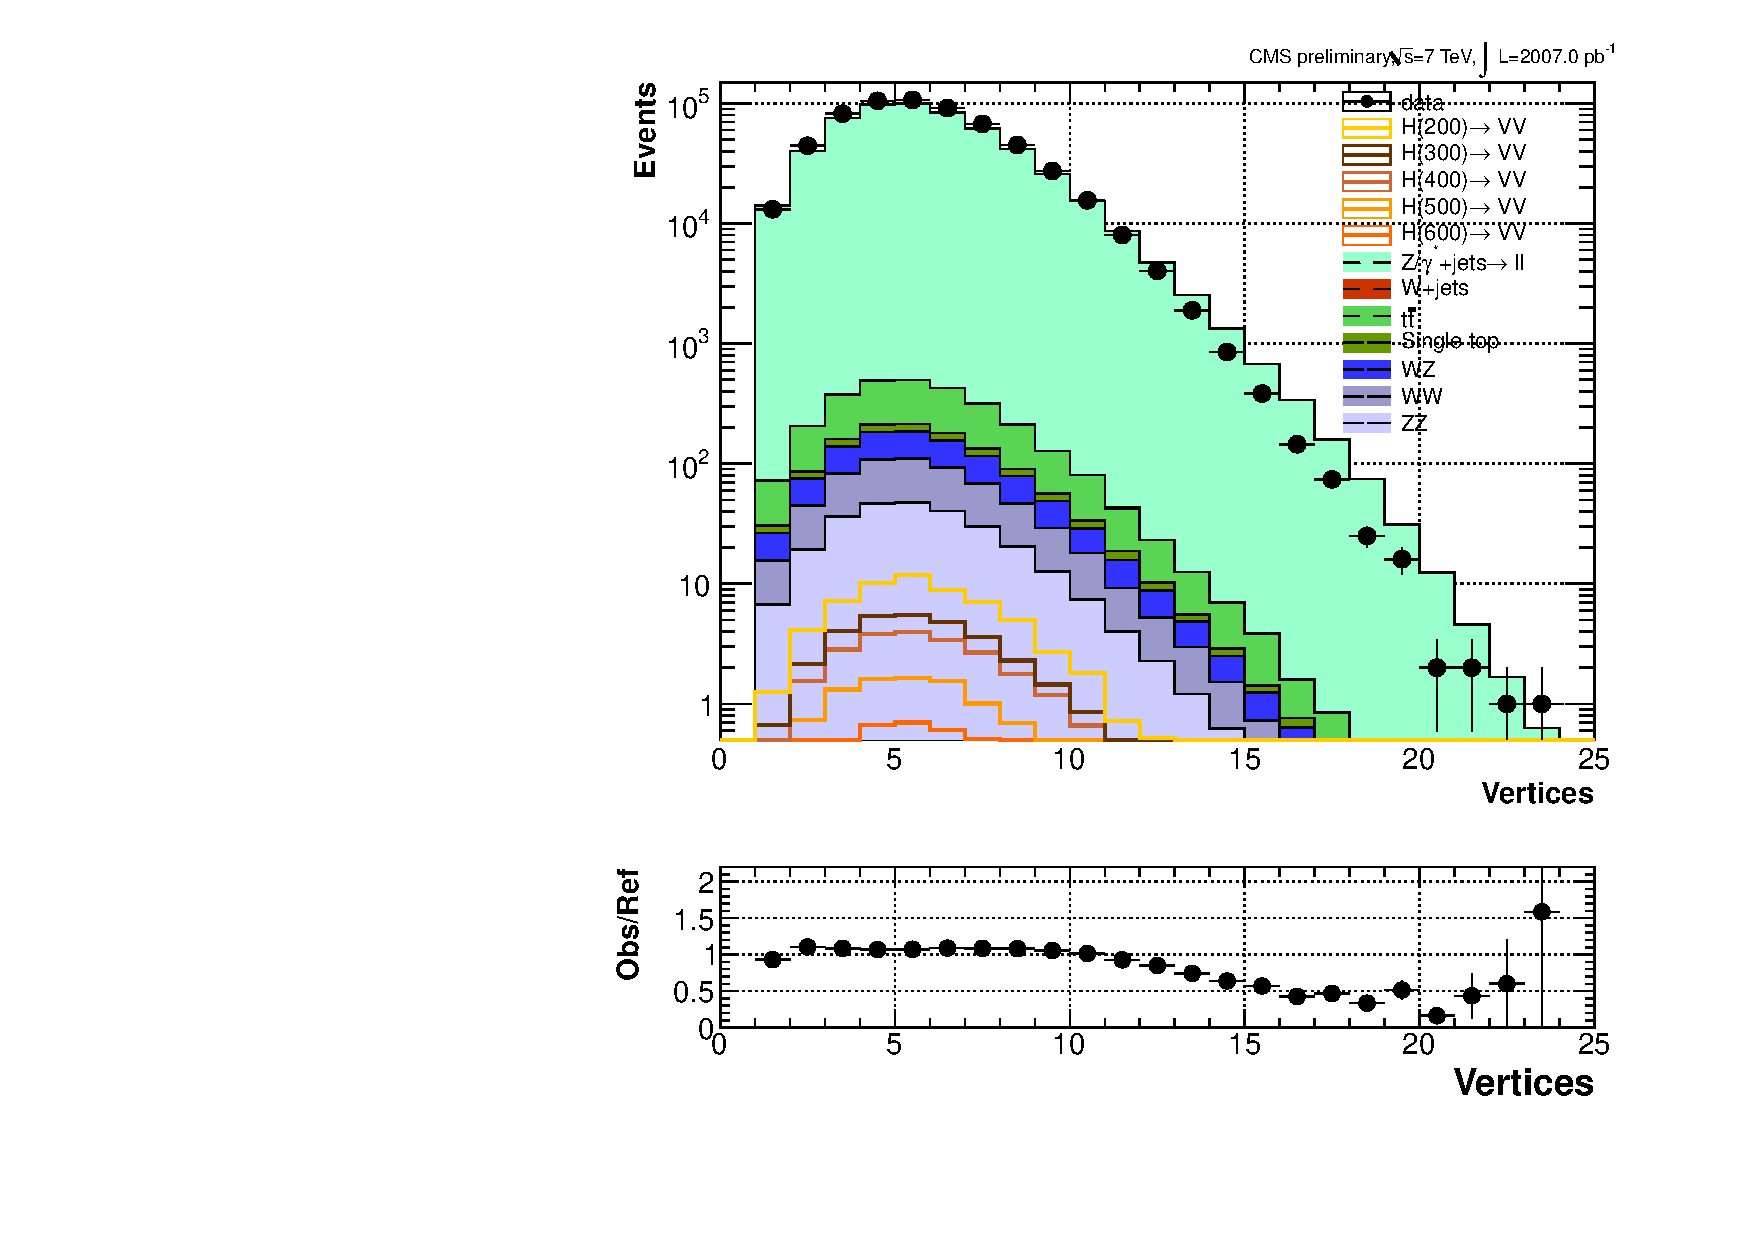
\includegraphics[width=0.4\textwidth]{img/mumu_ngoodvertex}
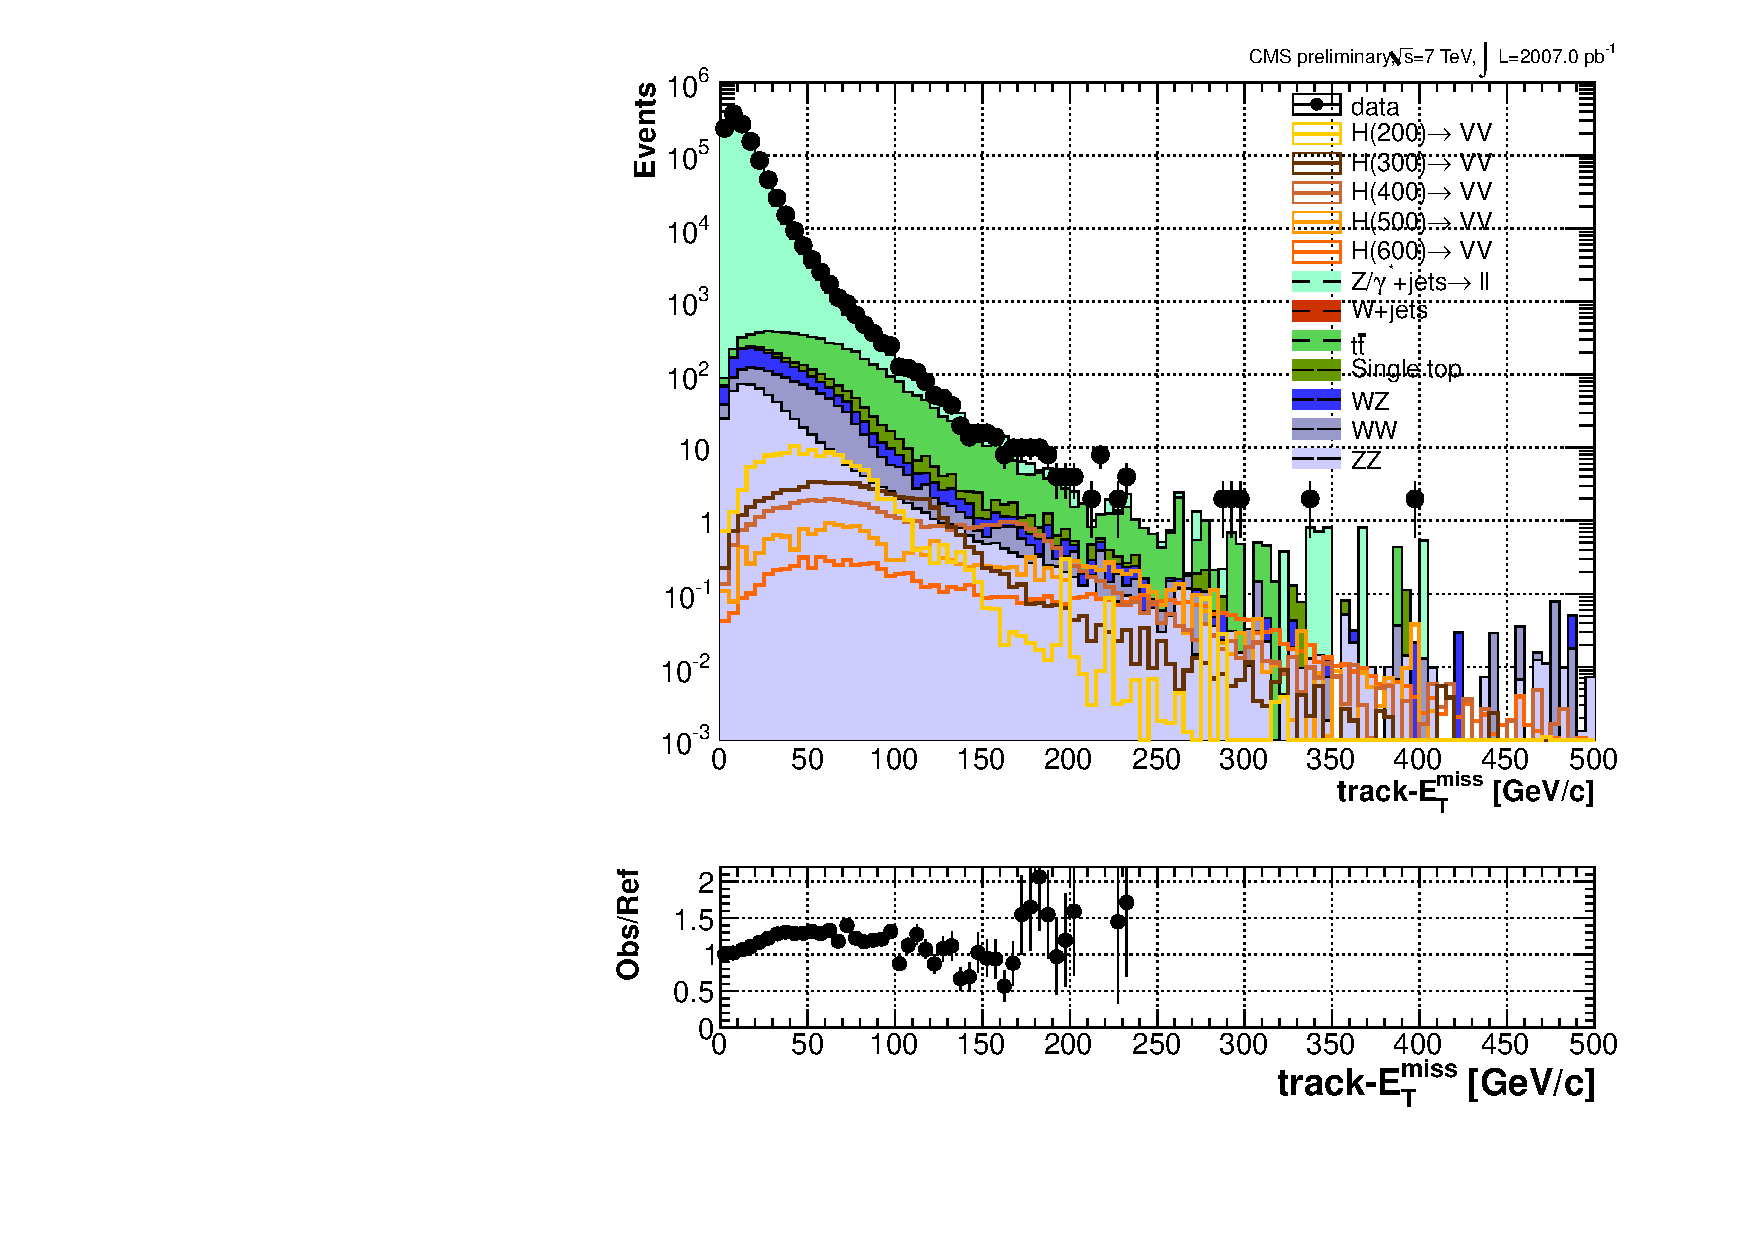
\includegraphics[width=0.4\textwidth]{img/mumu_trkmet}
\caption{Distribution of the vertex multiplicity ({\em left}) and the transverse momentum resulting from the sum of all charged particle-flow candidates associated to the primary vertex of the event ({\em right}).
The bottom plots show the ratio between the total \MC prediction and the observed data.}
\label{fig:vertexcontrol}
\end{center}
\end{figure}




%%% LEPTONS
\item[Leptons] leptons (electrons or muons) are required to be reconstructed with at least $p_T>$5~GeV/c and $|\eta|<$2.5 (2.4) for electrons (muons). 

Electrons reconstructed in the ECAL barrel to endcap transition are not considered for this study in order to reduce the contamination from fakes and to 
minimize the impact of mismeasurement of the lepton energies which translates to a mismeasurement of the missing transverse energy of the event.
The impact parameter of the electron track is required to be consistent with prompt production from the beam spot within $|d_0|<$0.04~cm.
Non-prompt electrons, from photon conversions in the tracker material, are vetoed by geometric requirements
applied on partner tracks (dist$<$0.02~cm and $\Delta\cot\theta<$0.02) and by requiring a maximum of 1 lost tracker hit. 
For each electron it is also required that no tracker or global muon with at least 10 tracker hits is found within a $\Delta R<$0.1 of the reconstructed electron.
Electron identification relies on a simple cut based identification algorithm 
which depends on the supercluster shape, its alignment with the track which is associated to electron and H/E.
The electron-id cuts are tuned specifically for each ECAL region (barrel and endcap) in order to yield 
an expected efficiency for the reconstruction of electrons from $W\rightarrowe\nu$ decays.
Details on the VBTF specific requirements can be found in~\cite{CMS-TWIKI-VBTF11}.
For this study we require at pre-selection that the VBTF-95 working point is verified. 
For electron candidates to be considered as a leg of the dilepton candidate the verification of the VBTF-85 working point is further required
as well as having $p_T>$20~GeV/c. 
The choice on these electron-ids is trigger oriented, as the trigger identification requirements consist in looser versions of the VBTF requirements.

Muon identification is mainly based on the $\chi^2$ fit of the global track and on the number of hits in the tracker and muon stations.
Loose muons are required to verify the TrackerMuonArbitrated criteria, i.e. to be tracker muons, 
and to be consistent with prompt production from the beam spot within $|d_0|<$0.02~cm.
Basic tracker quality requirements are also imposed, namely that : $\chi^2/ndof<$10 and at least 11 tracker hits are used for the inner track fit.
In order to be considered as a leg of the dilepton candidate the muons are furthermore required 
to have 1 hit in the muon chambers and to verify the TMLastStationAngTight arbitration and have $p_T>$20~GeV.

The leptons from signal are expected to be well isolated in the event.
The isolation can be quantified relatively to the transverse momentum of the lepton by
sum of the momenta of the particles reconstructed in a cone of $\Delta R<0.3$ built around the lepton candidate.
The following measurement of the relative isolation is used, $I_{rel}$:

\begin{equation}
I_{rel}=\frac{I_{photons}+I_{neutral~hadrons}+I_{charged~hadrons}}{p_T}
\label{eq:reliso}
\end{equation}

where each $I$ represents the sum of the transverse momenta of the photons, neutral hadrons and charged hadrons reconstructed inside the isolation cone.
Loose electrons and muons are required to have $I_{rel}<$0.5. 
Electrons or muons are considered as legs of the dilepton candidate if they have $I_{rel}<0.1$.
In App.~\cite{sec:app:leptonisolation} the lepton isolation is discussed in further detail.


%%% DILEPTON
\item[Dilepton] for each event with at least 2 leptons selected in the previous conditions all dilepton pair candidates are examined.
The dilepton candidate is required to have an invariant mass compatible with a $Z$ boson decay, i.e. $|M-M_Z|<$15~GeV/c$^2$
and in case of ambiguity the pair with highest $\sum p_T$ is chosen.
No requirement is made on the charge of the leptons.
The reconstructed dilepton mass in the $Z$ boson acceptance window and the angle made by the two leptons in the transverse plane ($\Delta\phi$)
is shown in Fig~\ref{fig:dileptoncontrol}.

\begin{figure}[htp]
\begin{center}
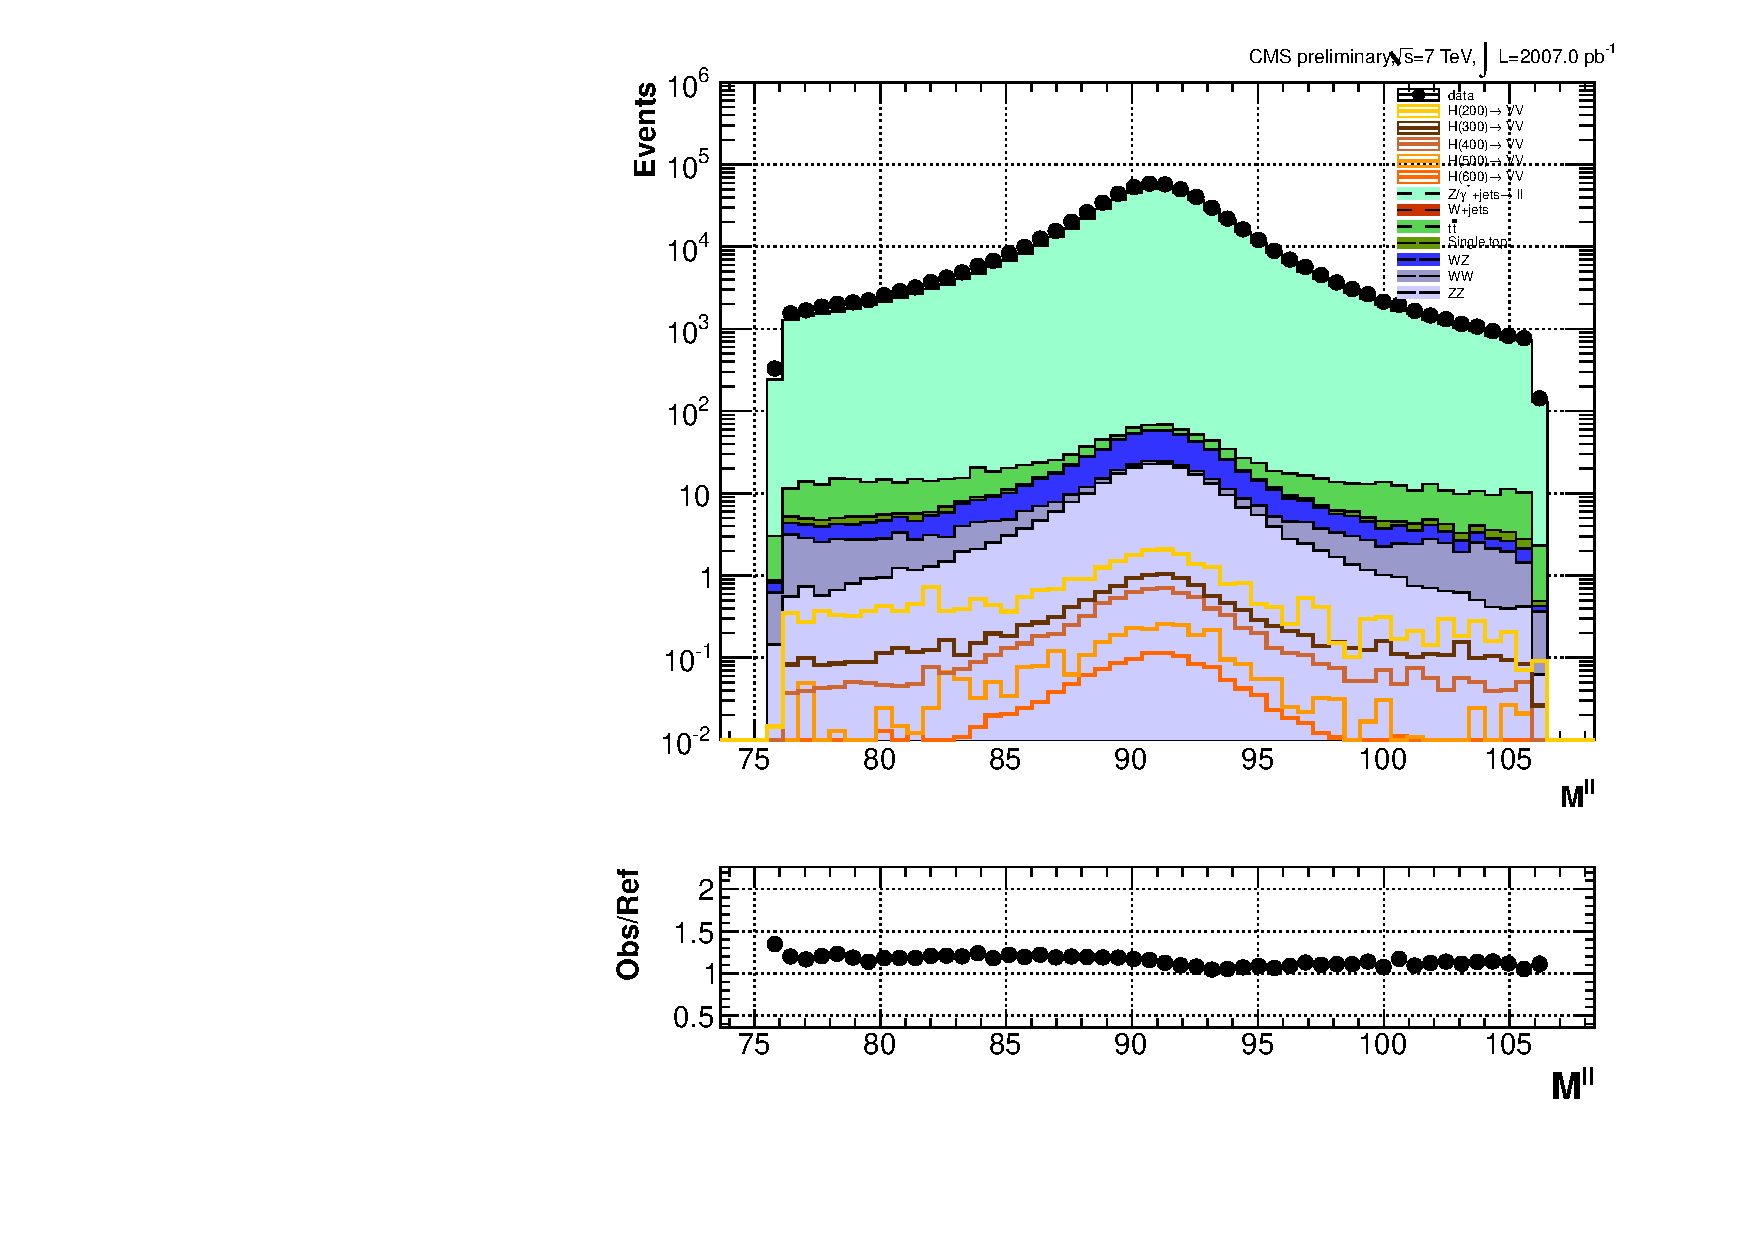
\includegraphics[width=0.4\textwidth]{img/mumu_recozmass}
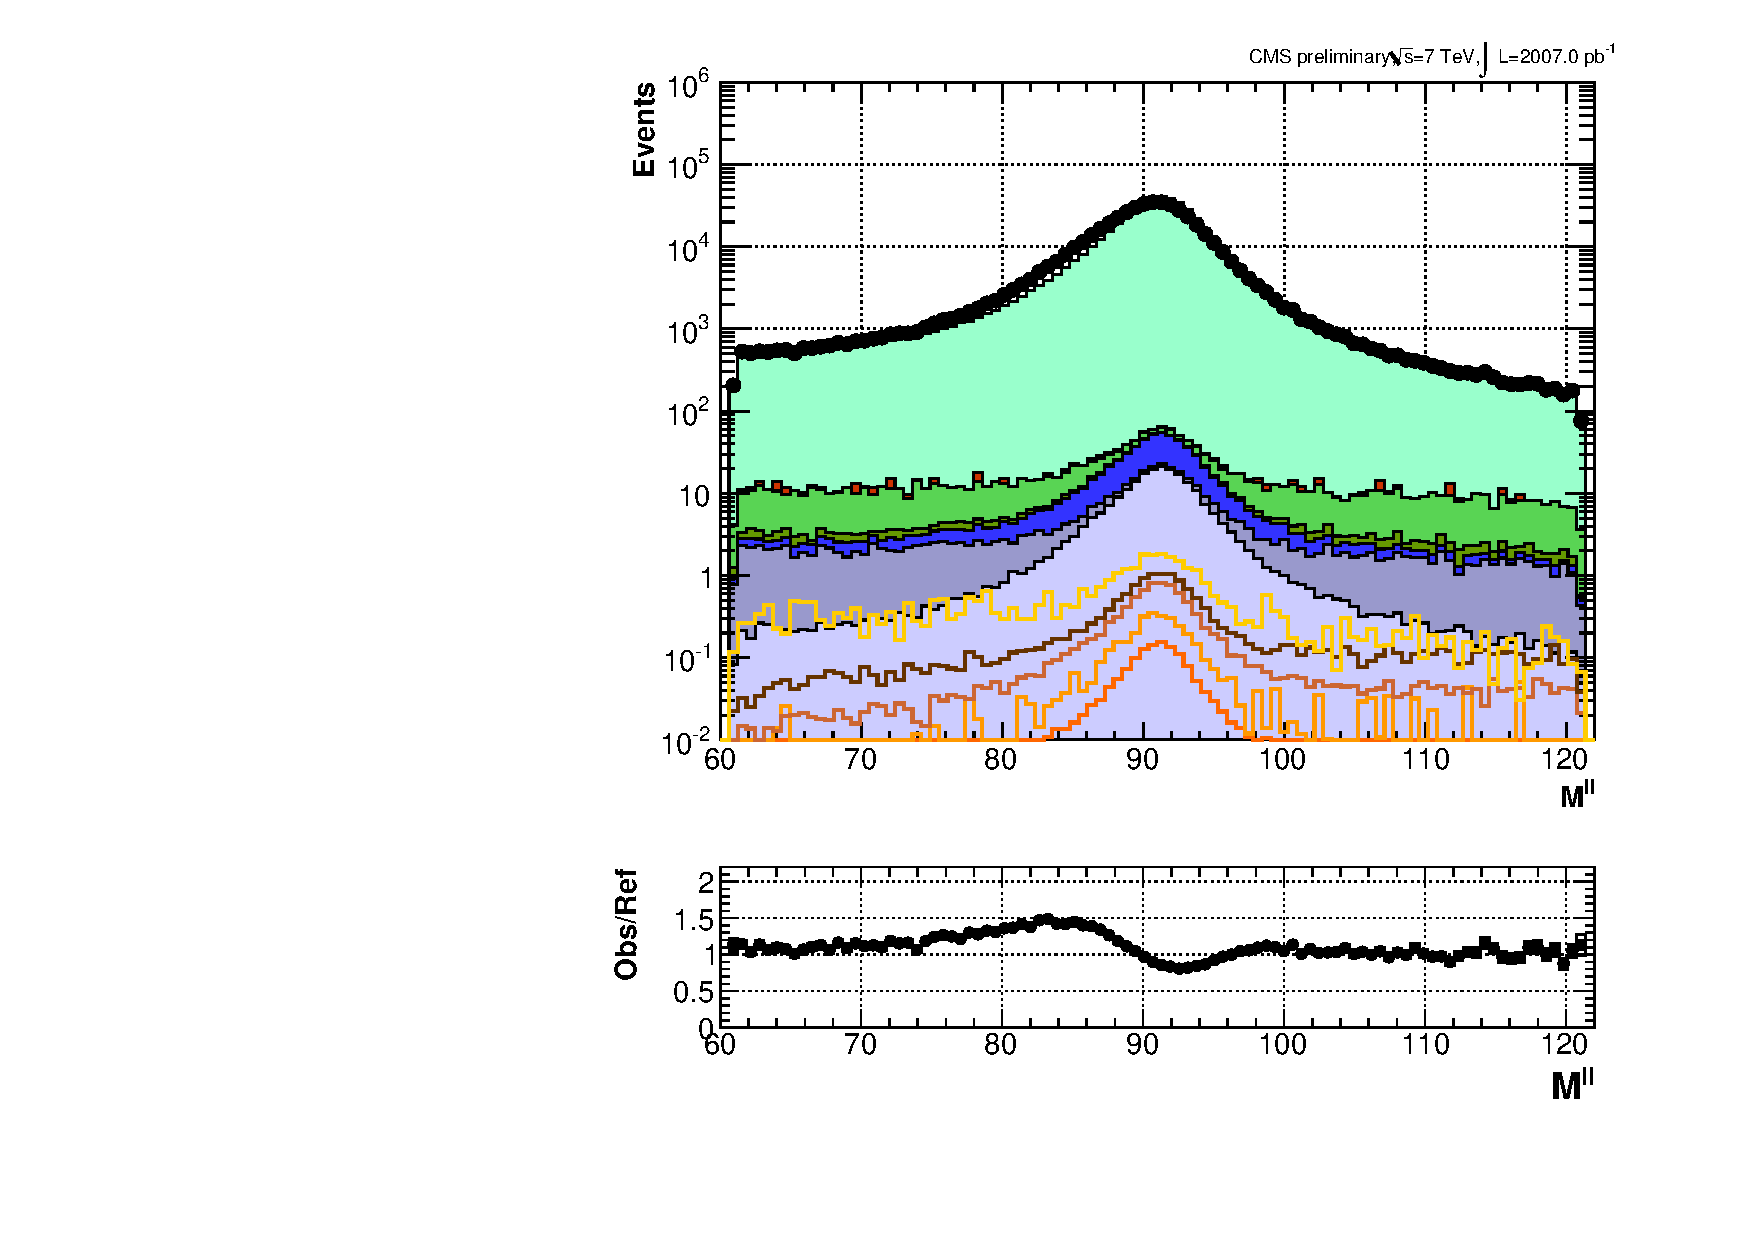
\includegraphics[width=0.4\textwidth]{img/ee_recozmass} \\
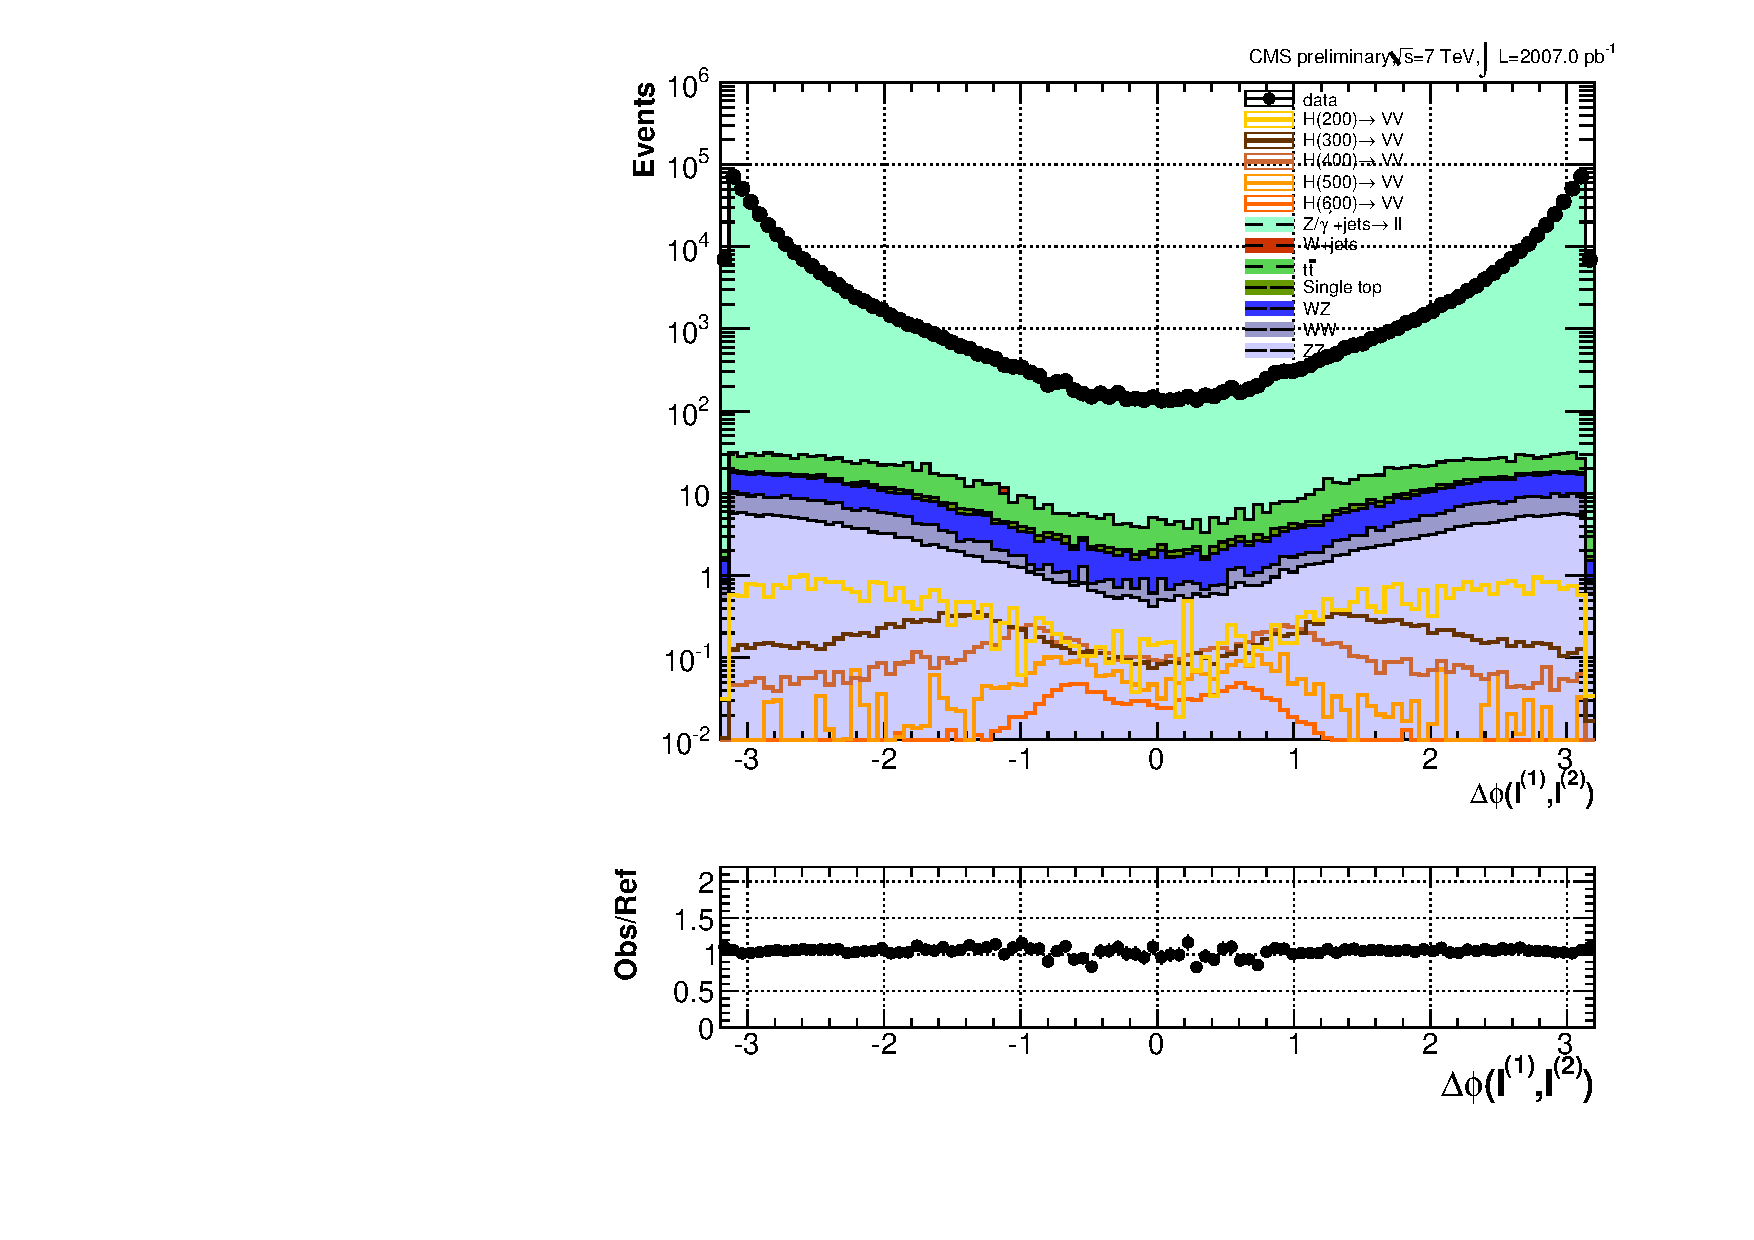
\includegraphics[width=0.4\textwidth]{img/mumu_recodphill}
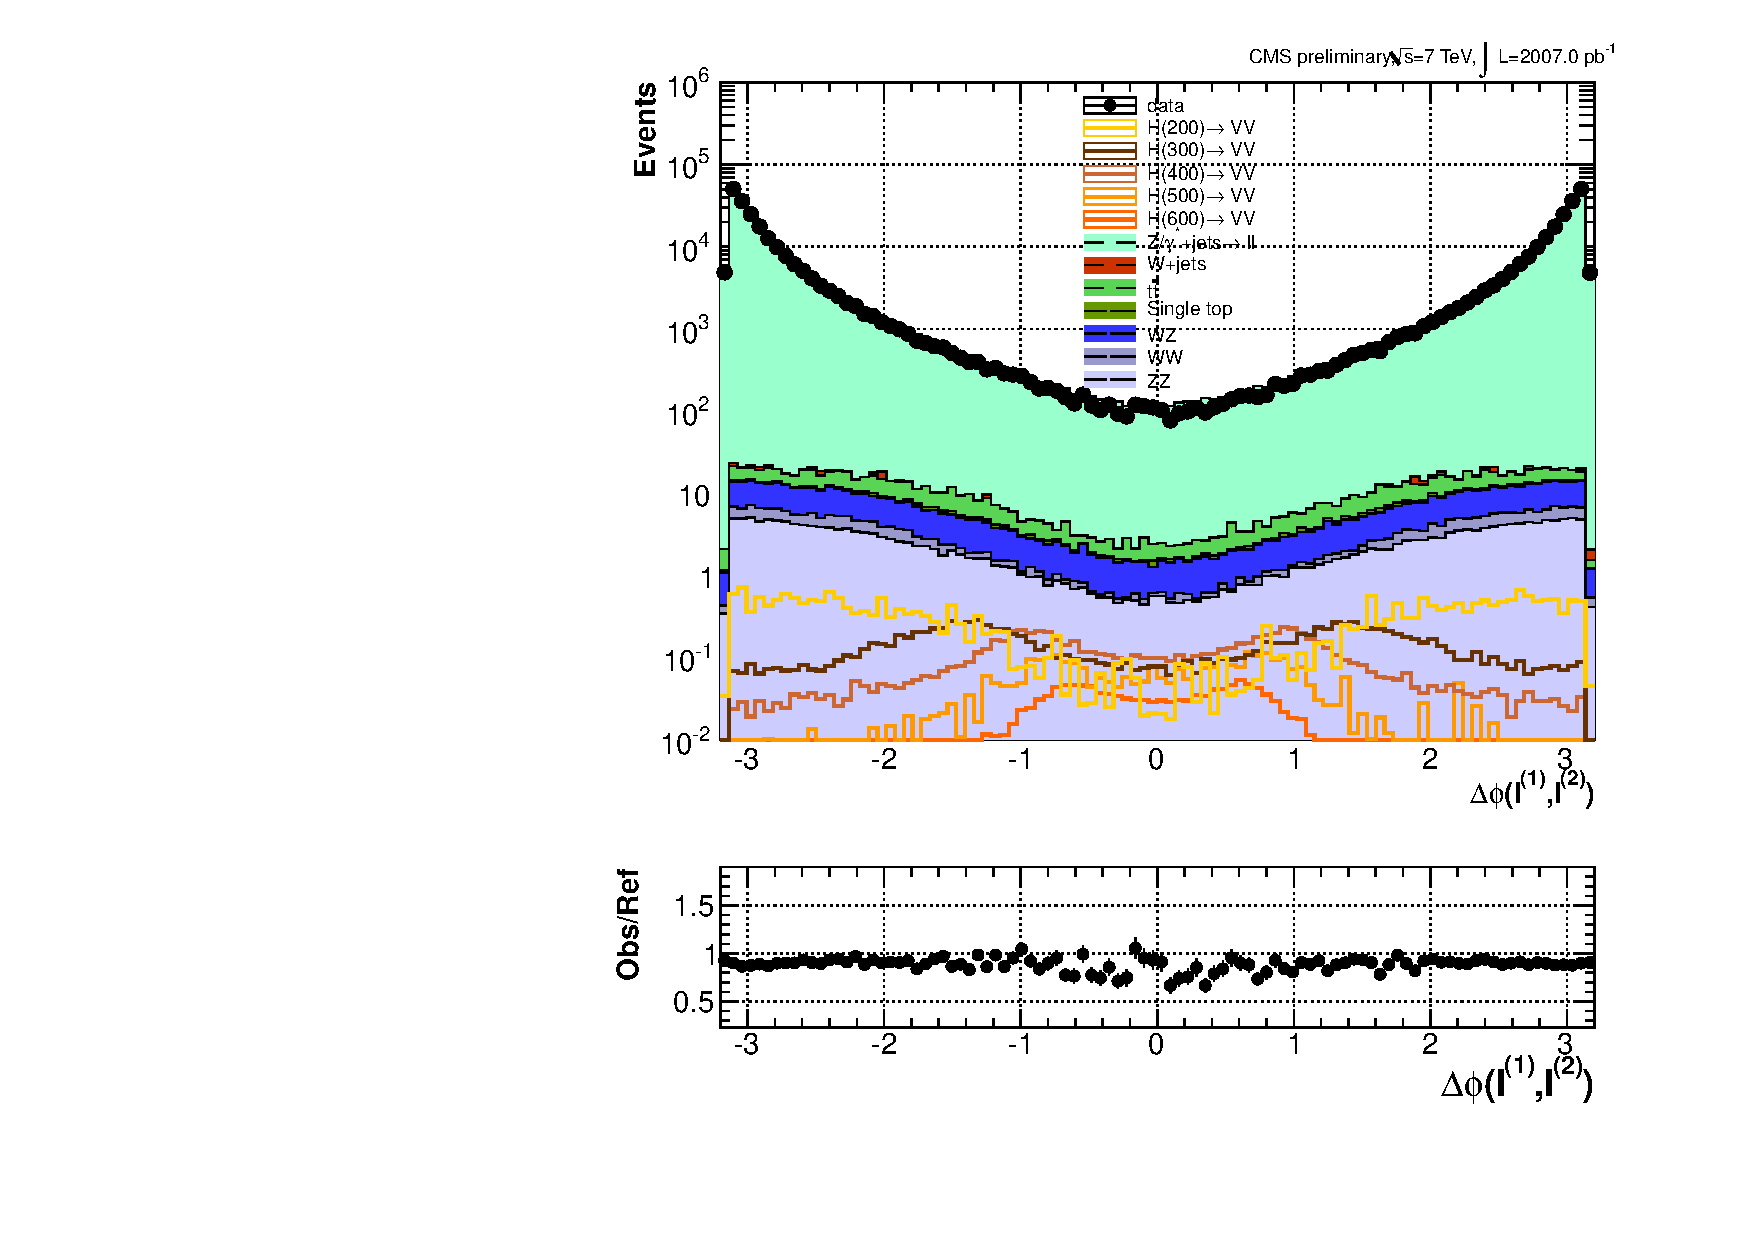
\includegraphics[width=0.4\textwidth]{img/ee_recodphill}
\caption{Lepton multiplicity distribution for di-muon ({\em left}) and di-electron ({\em right}) events with a mass compatible with the Z boson mass.}
\label{fig:dileptoncontrol}
\end{center}
\end{figure}

In order to reduce the contamination from multilepton events, produced from WZ and ZZ decays,
events are vetoed if containing another loosely selected electron or muon as described above.
The loose selection applied on the third lepton is expected to have a high efficiency for signal events($>$99.8\% for both channels).
The remainder of WZ and ZZ events are mostly due to fully hadronic decays of one of the vector bosons or to the decay of a Z boson to neutrinos.
A slight excess of events with more than 2 muons is observed in data as shown in Fig~\ref{fig:thirdleptonveto}
most probably related to a higher lepton fake rate than the one modelled by the \MC.
Notice also that at this point no data-driven correction for the lepton efficiencies has been applied to correct further the \MC.

\begin{figure}[htp]
\begin{center}
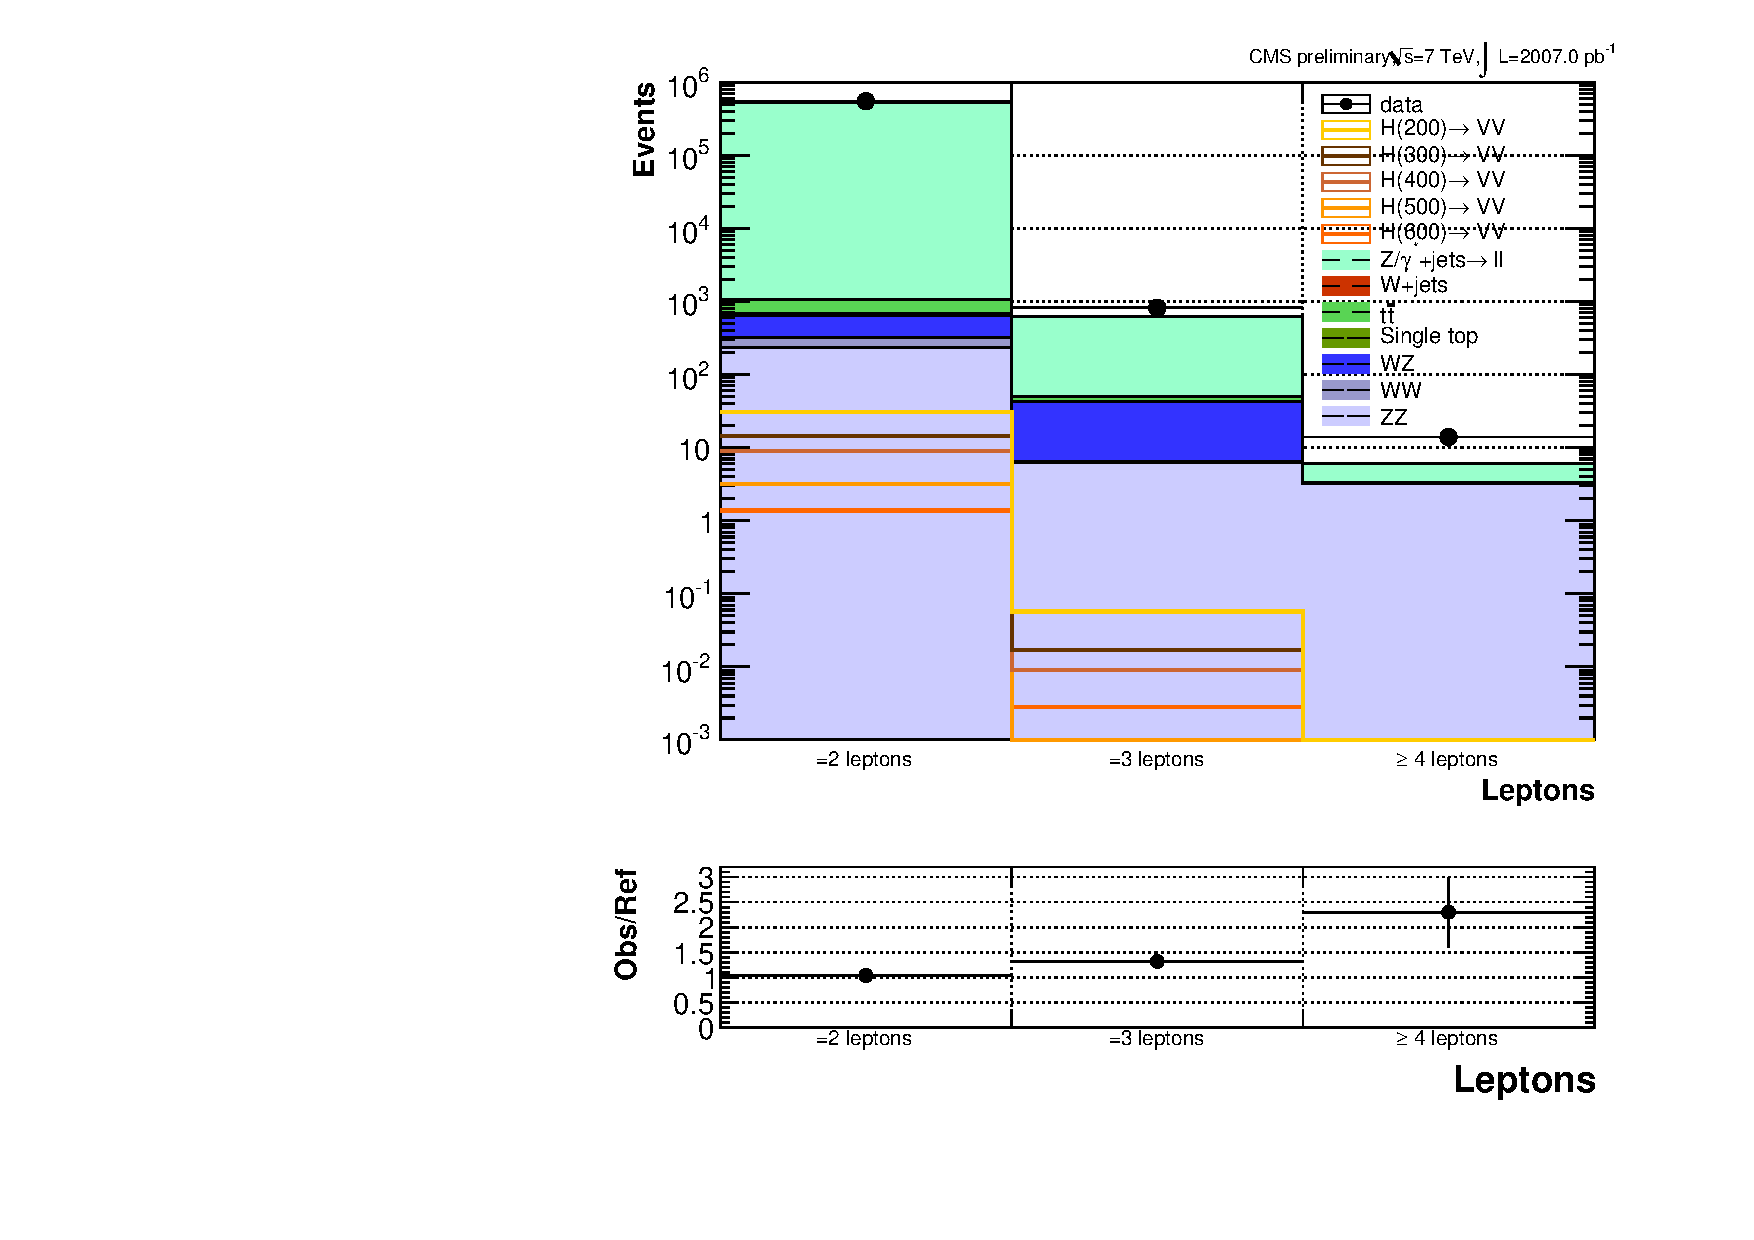
\includegraphics[width=0.4\textwidth]{img/mumu_nleptons}
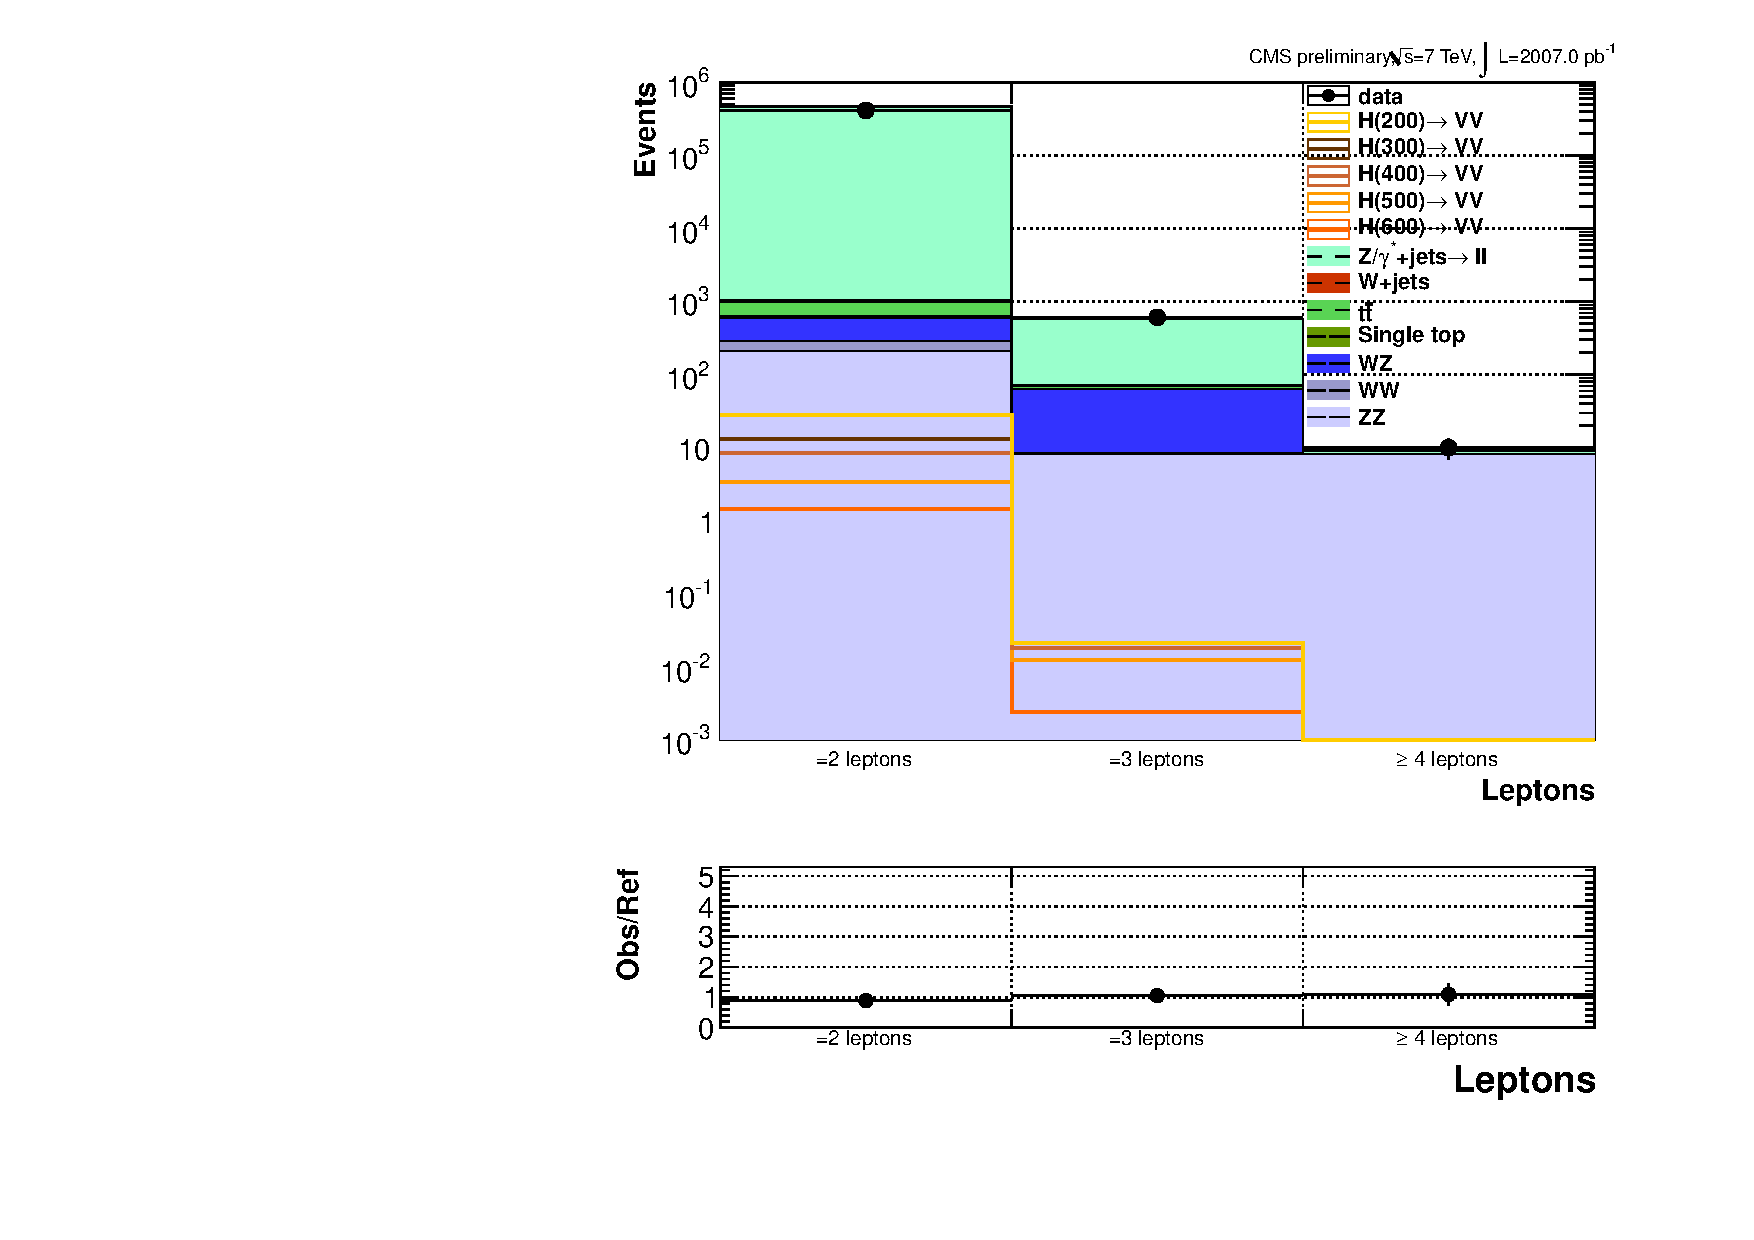
\includegraphics[width=0.4\textwidth]{img/ee_nleptons}
\caption{Lepton multiplicity distribution for di-muon ({\em left}) and di-electron ({\em right}) events with a mass compatible with the Z boson mass.}
\label{fig:thirdleptonveto}
\end{center}
\end{figure}


%%% JETS
\item[Jets] are reconstructed with the anti-$k_T$ algorithm with a cone of $R=0.5$ are selected with $p_T>$15~GeV/c and $|\eta|<5.0$.
The loose jet id used to select the jets is based on the electromagnetic fraction of the jets among other variables. 
The jet multiplicity distribution obtained after the dilepton selection is shown in Fig.~\ref{fig:jetmult} for jets found inside the tracker acceptance region only.
A good agreement is found between data and \MC prediction.
Jets with $|\eta|>2.5$ are used for the VBF specific selection which will be discussed in more detail in Sec.~\ref{sec:higgssearch}.

\begin{figure}[htp]
\begin{center}
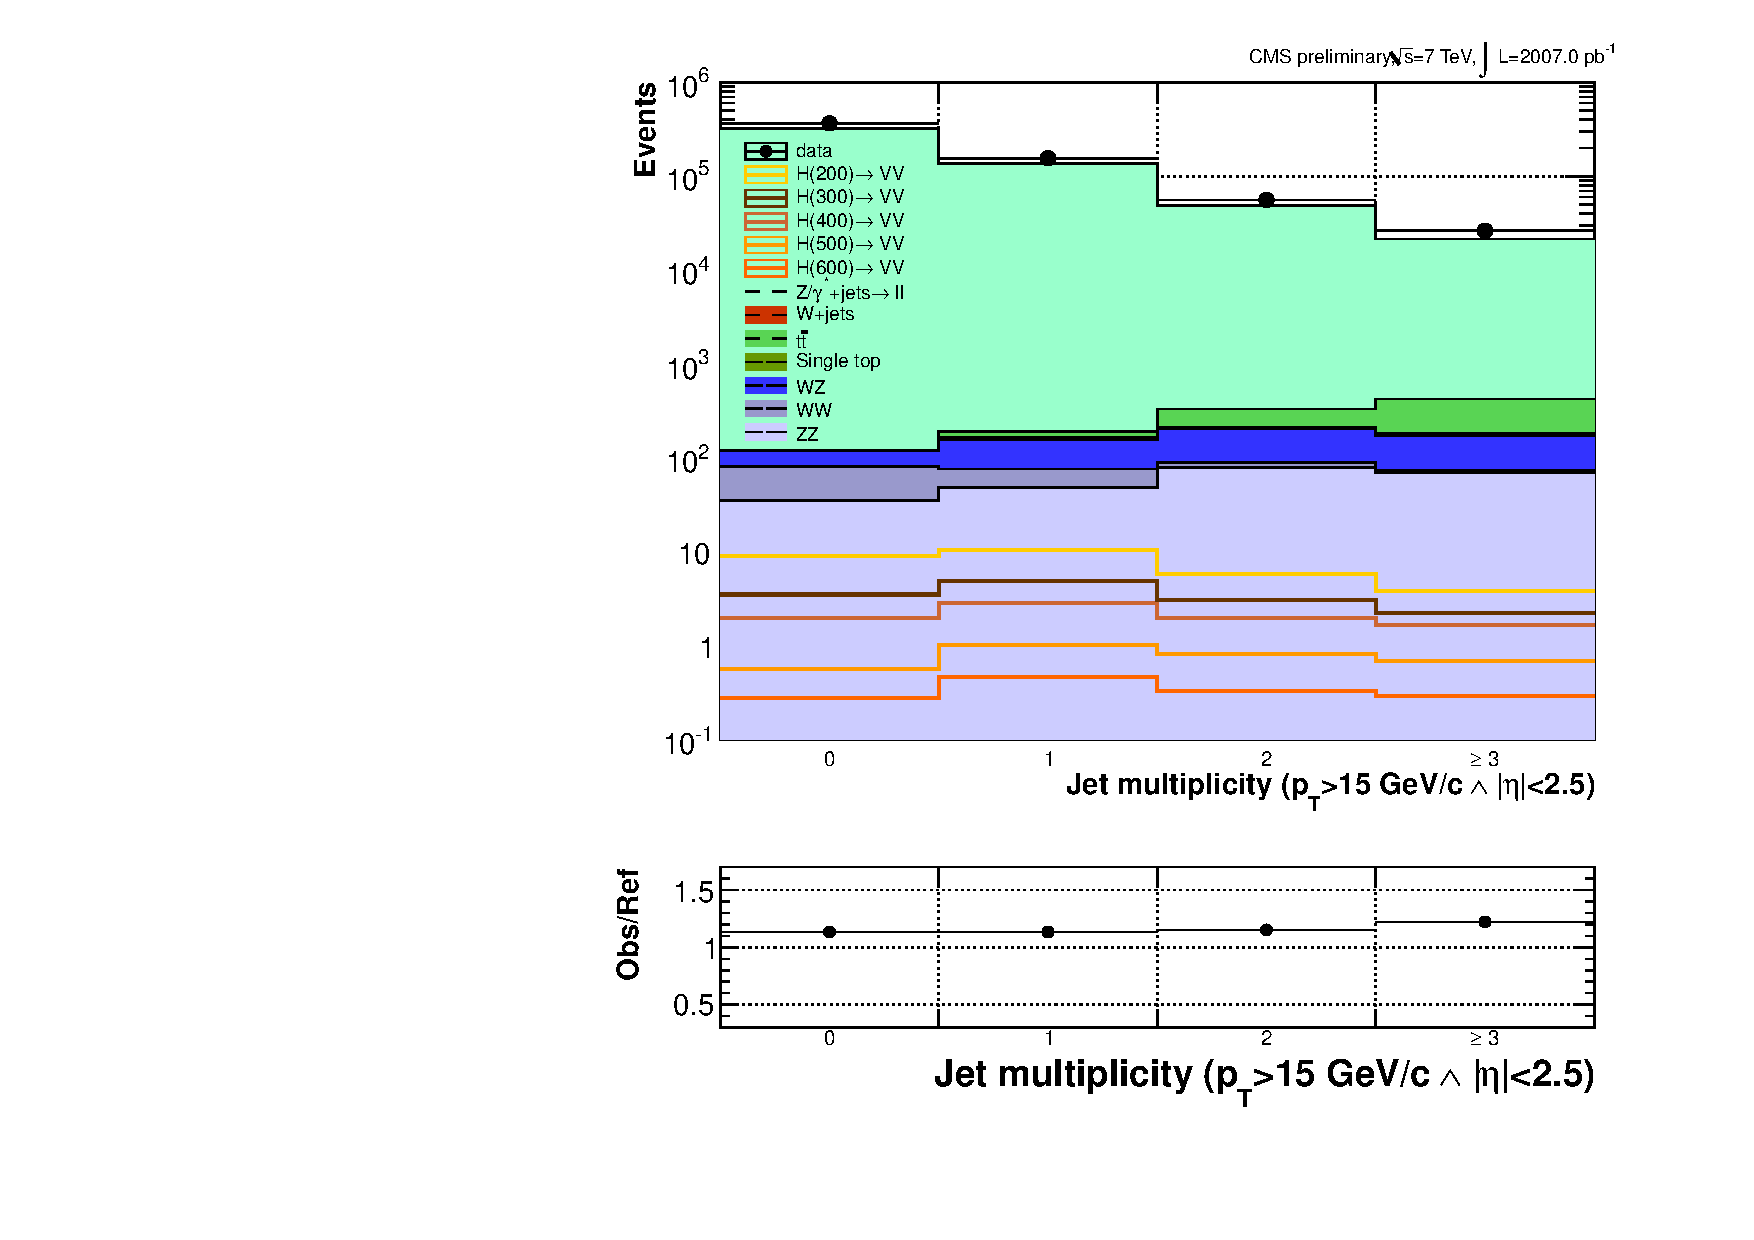
\includegraphics[width=0.4\textwidth]{img/mumu_njets}
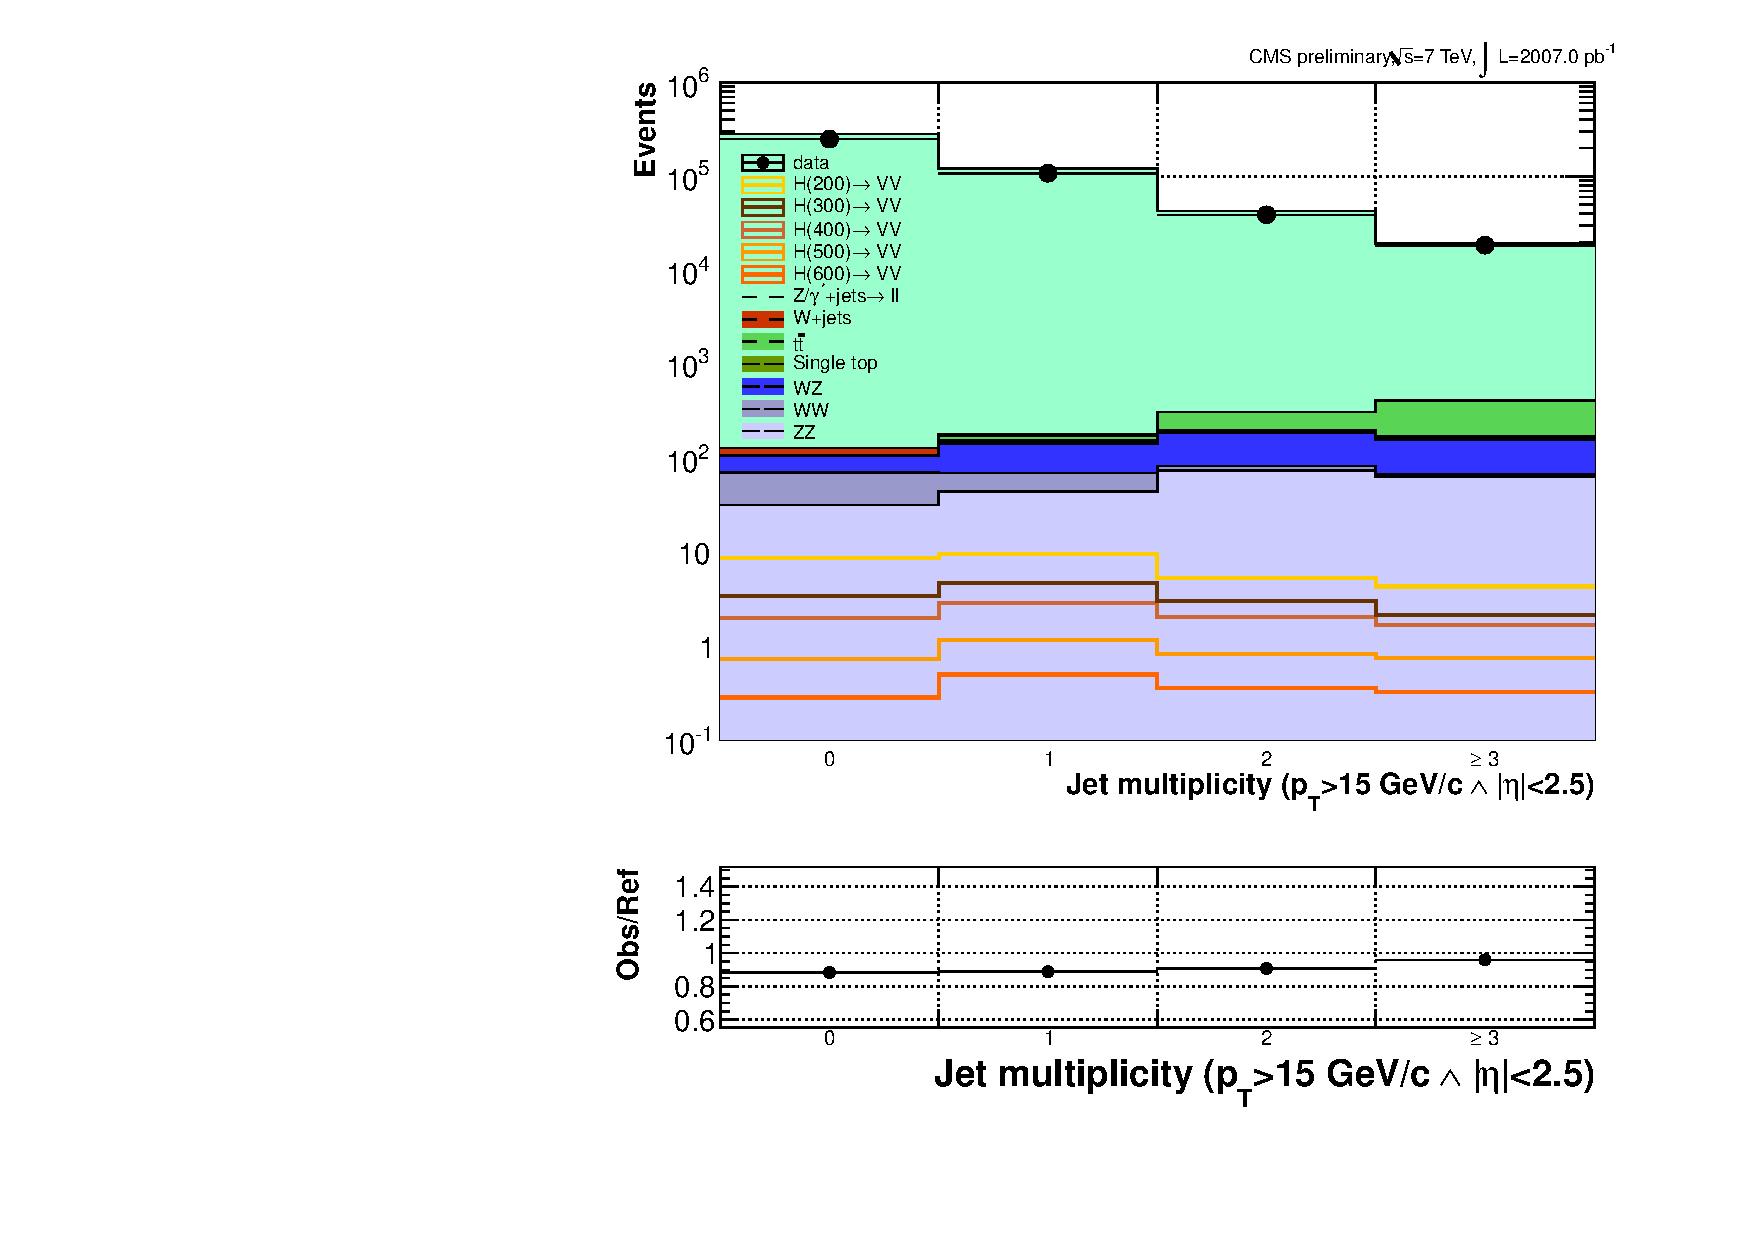
\includegraphics[width=0.4\textwidth]{img/ee_njets}
\caption{Jet multiplicity distribution in di-muon ({\em left}) and di-electron ({\em right}).}
\label{fig:jetmult}
\end{center}
\end{figure}

In order to reduce the contamination from processes which produce heavy flavor jets such as \ttbar, single top, vector boson + heavy quarks production, b-tagging algorithms are used.
The jet-B probability (JBP) and the simple secondary vertex high efficiency (SSVHE) taggers are used for this purpose. 
Details of these algorithms and their performance can be found in~\cite{CMS-PAS-BTV-11-002}. The JBP algorithm is chosen
as it is expected to provide the highest efficiency in \ttbar events for a mistag rate of 10\% (loose working point).
The SSVHE tagger is used to complement the JBP tagger as it is designed for higher purity of $b$-jet identification and can therefore
increase the $b$-tagging efficiency without leading to a significant increase of the mistag rate. 
Events with a jet with $p_T>$30~GeV/c, tagged with the loose working point of the JBP algorithm or with the medium working point of the SSVHE algorithm, are rejected. 
This choice is made after optimizing the efficiency of the rejection of the top contribution as summarized in Tab.~\ref{tab:btagoptim}.
Fig.~\ref{fig:btagging} shows the b-tag multiplicity distributions observed in di-muon and di-electron events using the combination of taggers just described.
A good agreement, within 10-15\% is found between data and \MC taking into account that at this point no data-driven correction scale factors for the $b$-tag and mistag rates have been applied.
The level of discrepancy observed is in fact compatible with the $\approx$ 10\% scale factor measured for the mistag rate~\cite{CMS-PAS-BTV-11-002}.
The usage of the data-derived scale factors for the $b$-tagging algorithms will be discussed in more detail in Sec.~\ref{subsec:systunc}.

\begin{table}[htp]
\caption{b-tag optimization using different algorithms and different combinations.
Top refers to the residual number of events expected from \ttbar and single top production.
Higgs refers to the number of events surviving the $b$-tagging veto for a mass of 200~GeV/c$^{2}$.
The yields include the di-muon and the di-electron channels for an integrated luminosity of 2007~pb$^{-1}$.
The last line shows the signal/background ratio used to optimize the choice of the $b$-tagging algorithm.
The taggers compared are Track Counting High Efficiency (TCHE), Jet B-probability (JBP) and Simple Secondary Vertex High Efficiency (SSVHE).
Two suffixes used for the different taggers denote the Loose and Medium working points.}
\label{tab:btagoptim}
\begin{center}
\begin{tabular}{lccccc} \hline\hline
\multirow{2}{*}{Process} & \multicolumn{5}{c}{Events accepted} \\
              & TCHEL          & JBPL      & SSVHEM   & TCHEL or SSVHEM & JBPL or SSVHEM \\\hline
Top           & 124.03         & 107.95    & 230.22   & 108.60          & 102.1          \\
Higgs (200)   & 50.97          & 51.97     & 55.31    & 50.74           & 51.77          \\\hline
S/B           & 0.41           & 0.48      & 0.24     & 0.47            & 0.51           \\
\hline\hline
\end{tabular}
\end{center}
\end{table}


\begin{figure}[htp]
\begin{center}
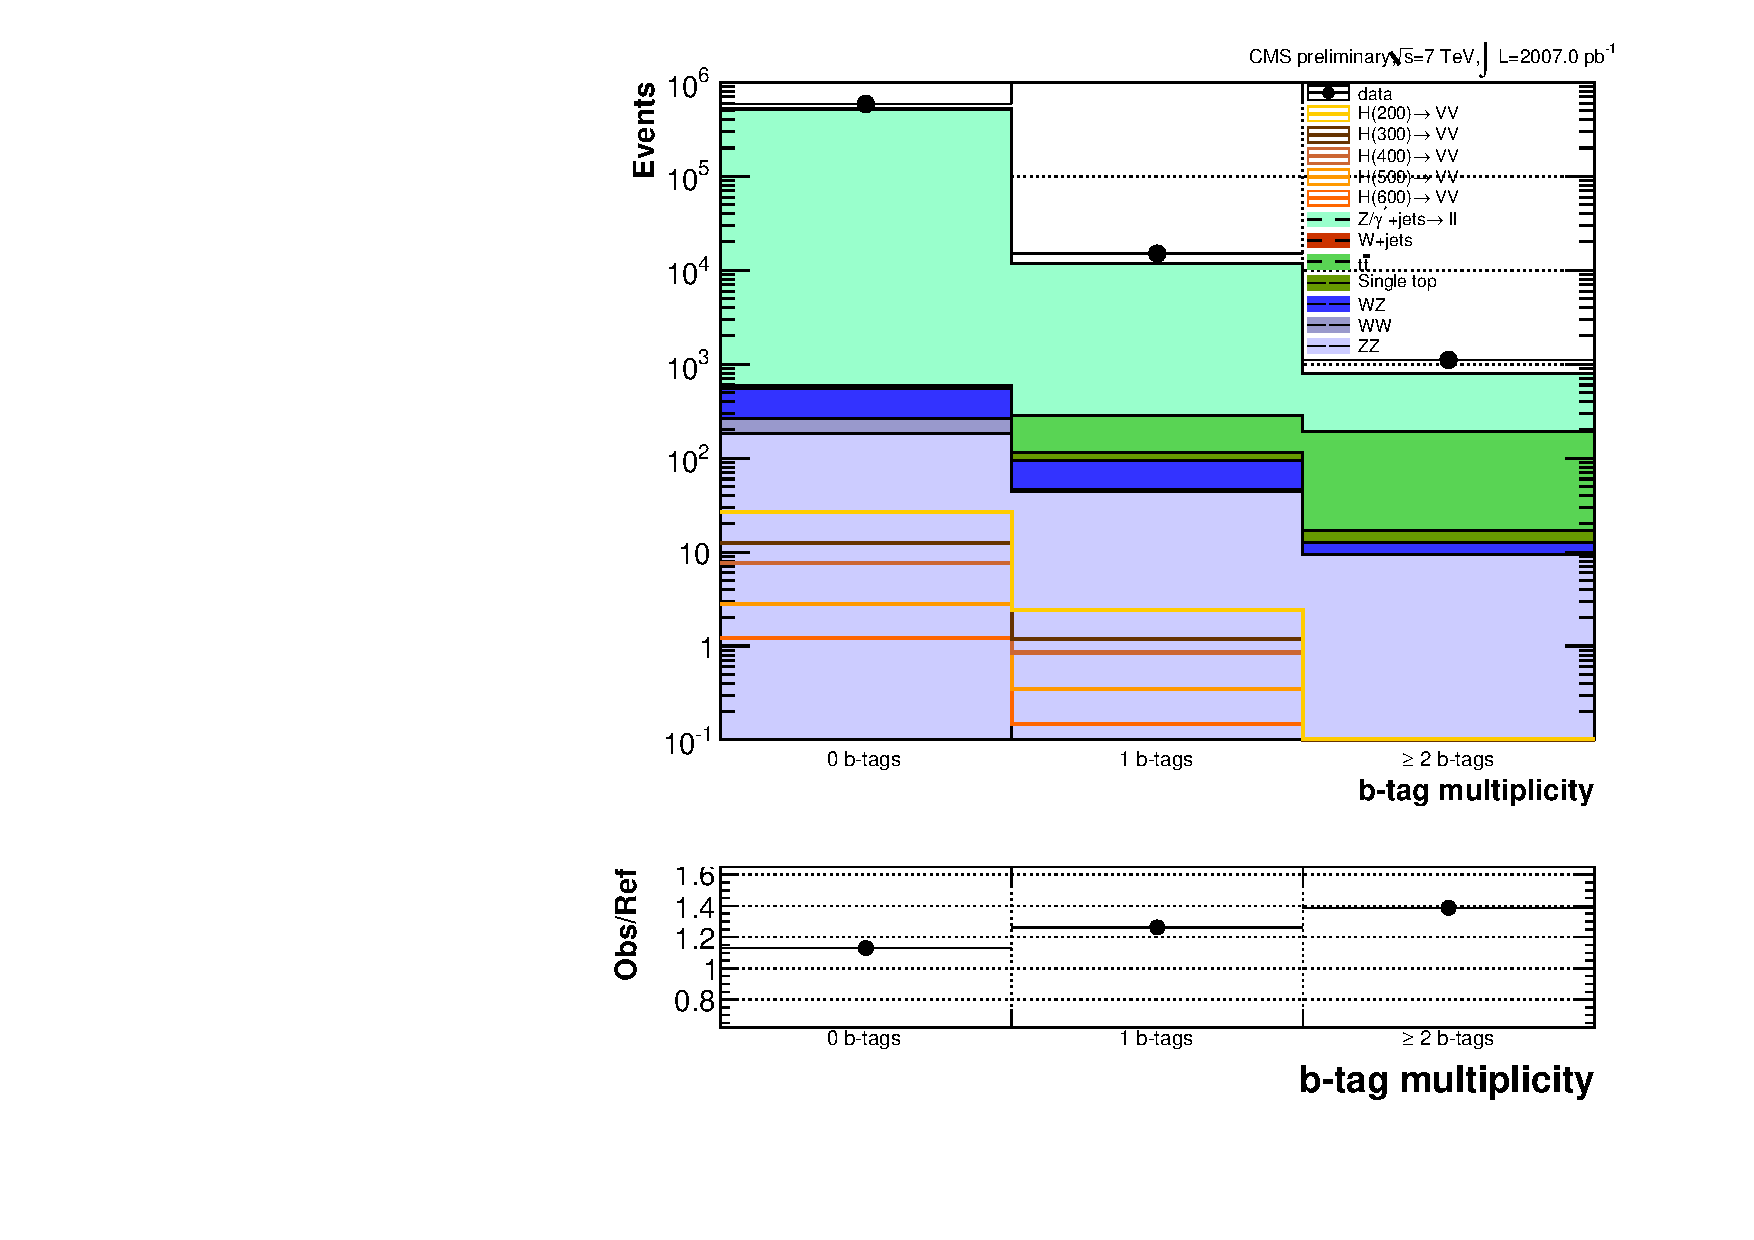
\includegraphics[width=0.46\textwidth]{img/mumu_nbtags}
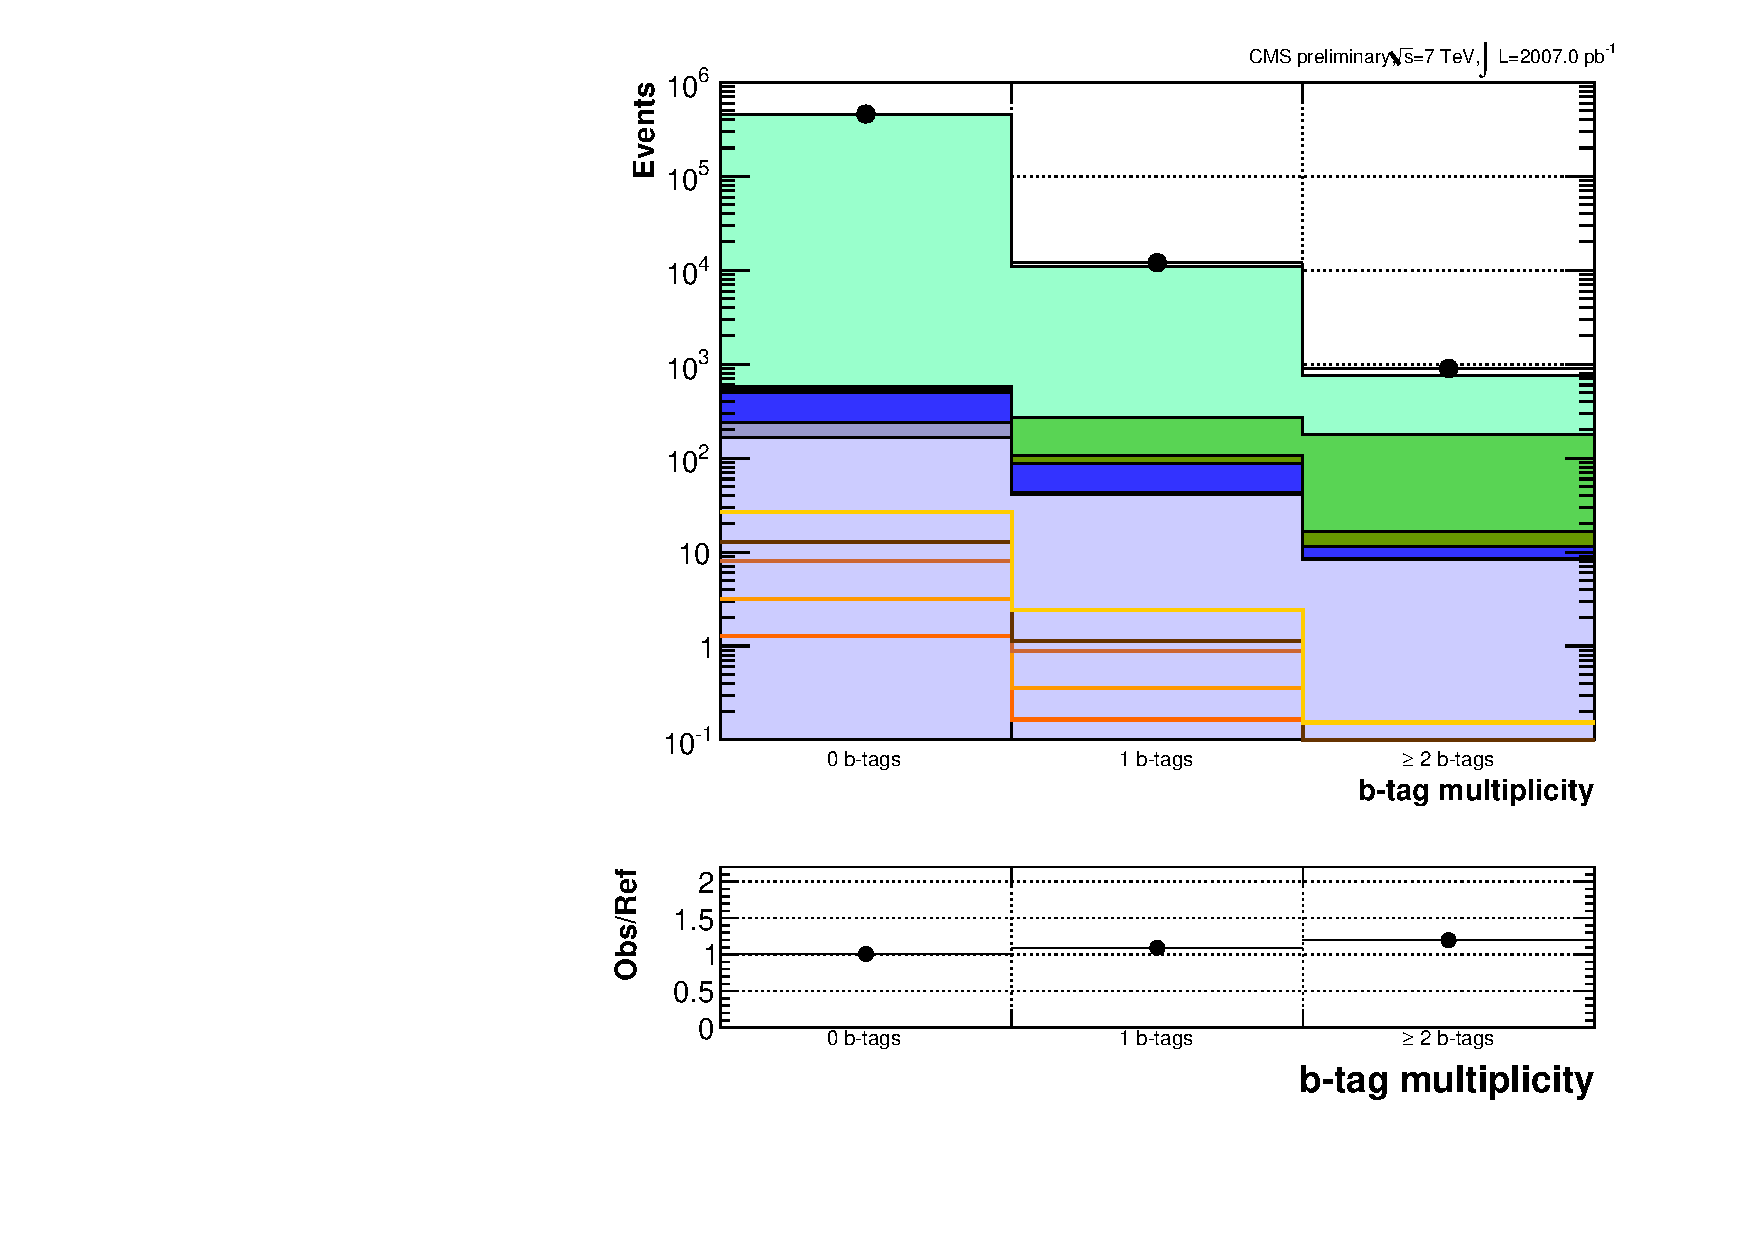
\includegraphics[width=0.46\textwidth]{img/ee_nbtags}
\caption{b-tag  multiplicity distribution in di-muon ({\em left}) and di-electron ({\em right}).}
\label{fig:btagging}
\end{center}
\end{figure}


%%% MET
\item[Missing transverse energy] particle flow based \MET is used. The \MET is built from the vectorial sum of the transverse momentum all particle flow reconstructed candidates.
The verification of the reconstruction of the missing transverse energy will be the subject of a detailed discussion in Sec.~\ref{sec:met}
and a specific \MET based selection will be proposed to reduce more efficienctly the contamination from $Z$ events with minimal contamination from pileup.
Fig.~\ref{fig:metcontrol} shows the distribution for the \MET after the $b$-jet veto has been applied. 
A wider resolution is observed in data with respect to the \MC prediction reinforcing the need to develop a detailed verification of its reconstruction
and a data-driven method to model the expected performance to remove $Z$ events.

\begin{figure}[htp]
\begin{center}
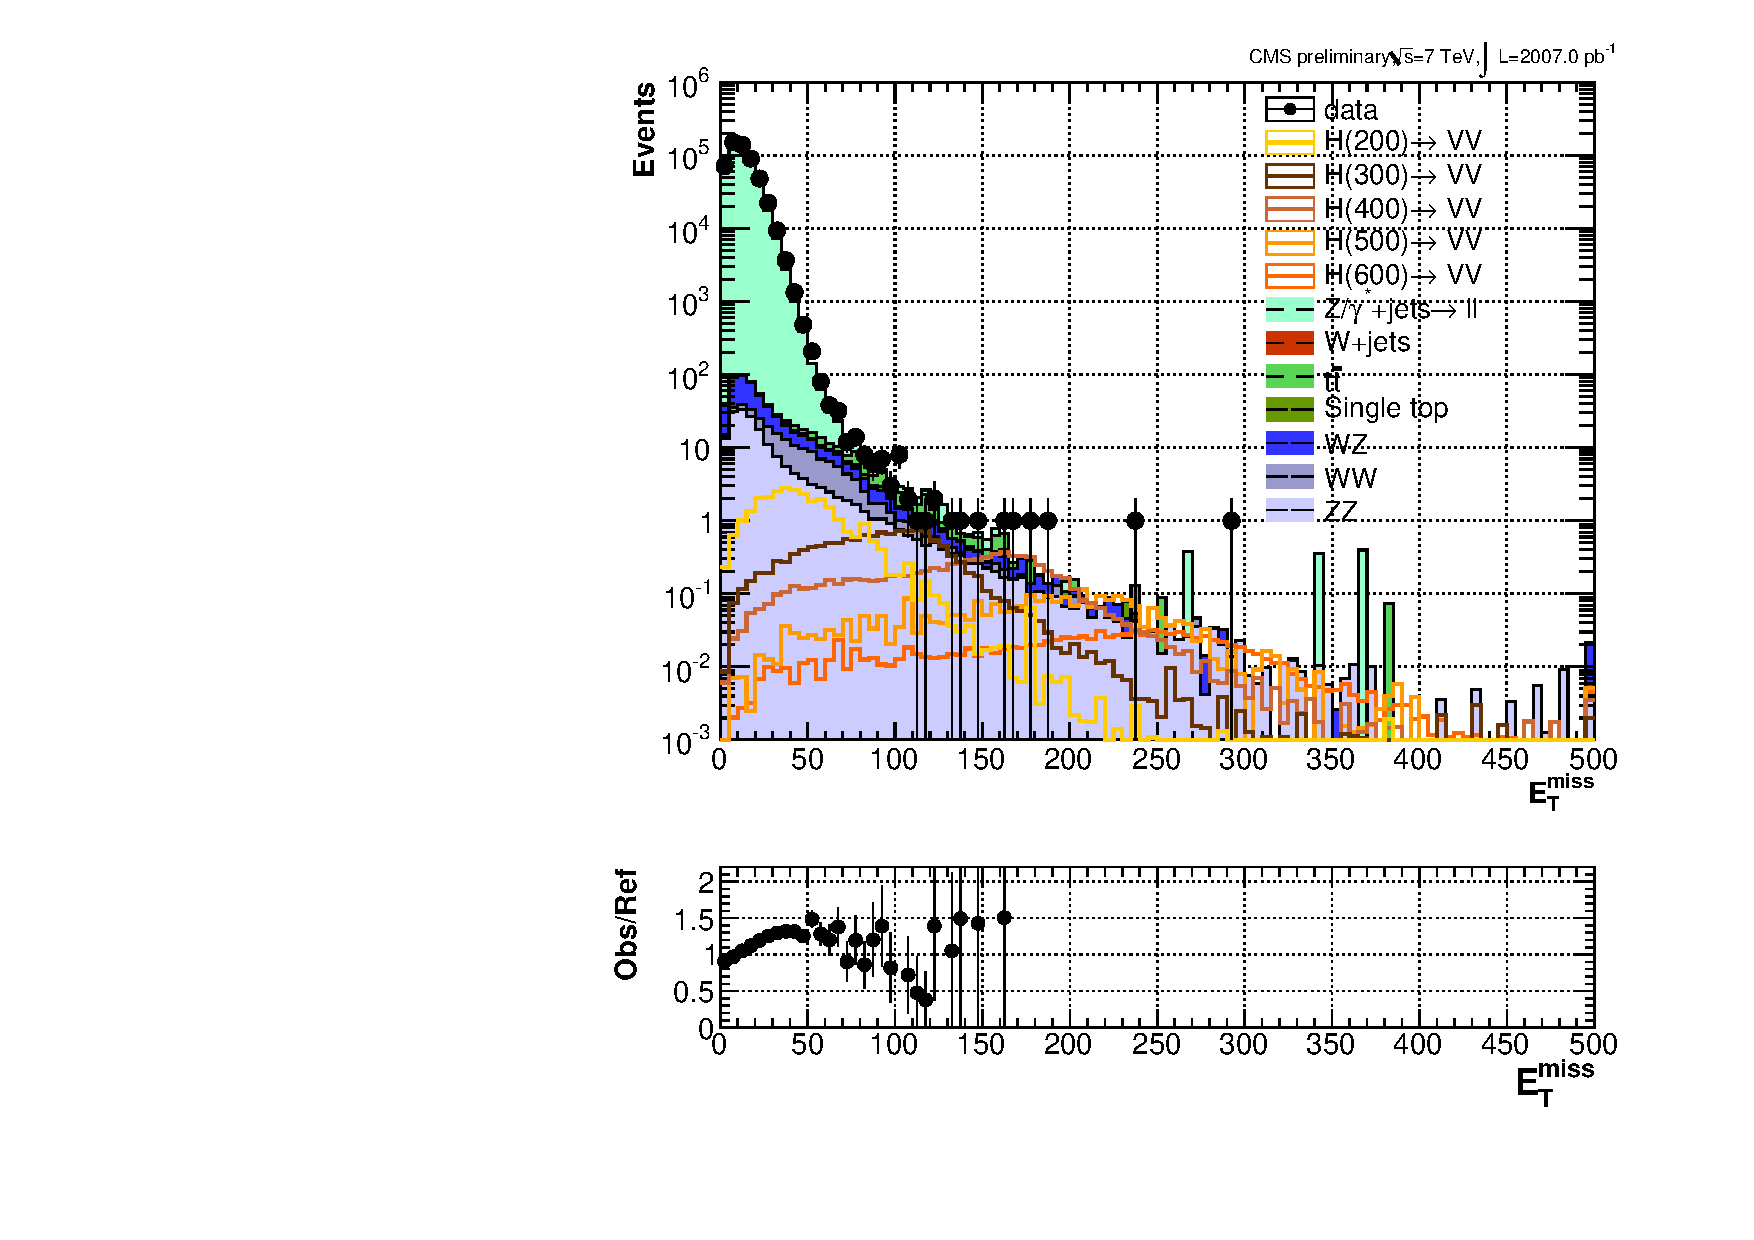
\includegraphics[width=0.46\textwidth]{img/mumu_met}
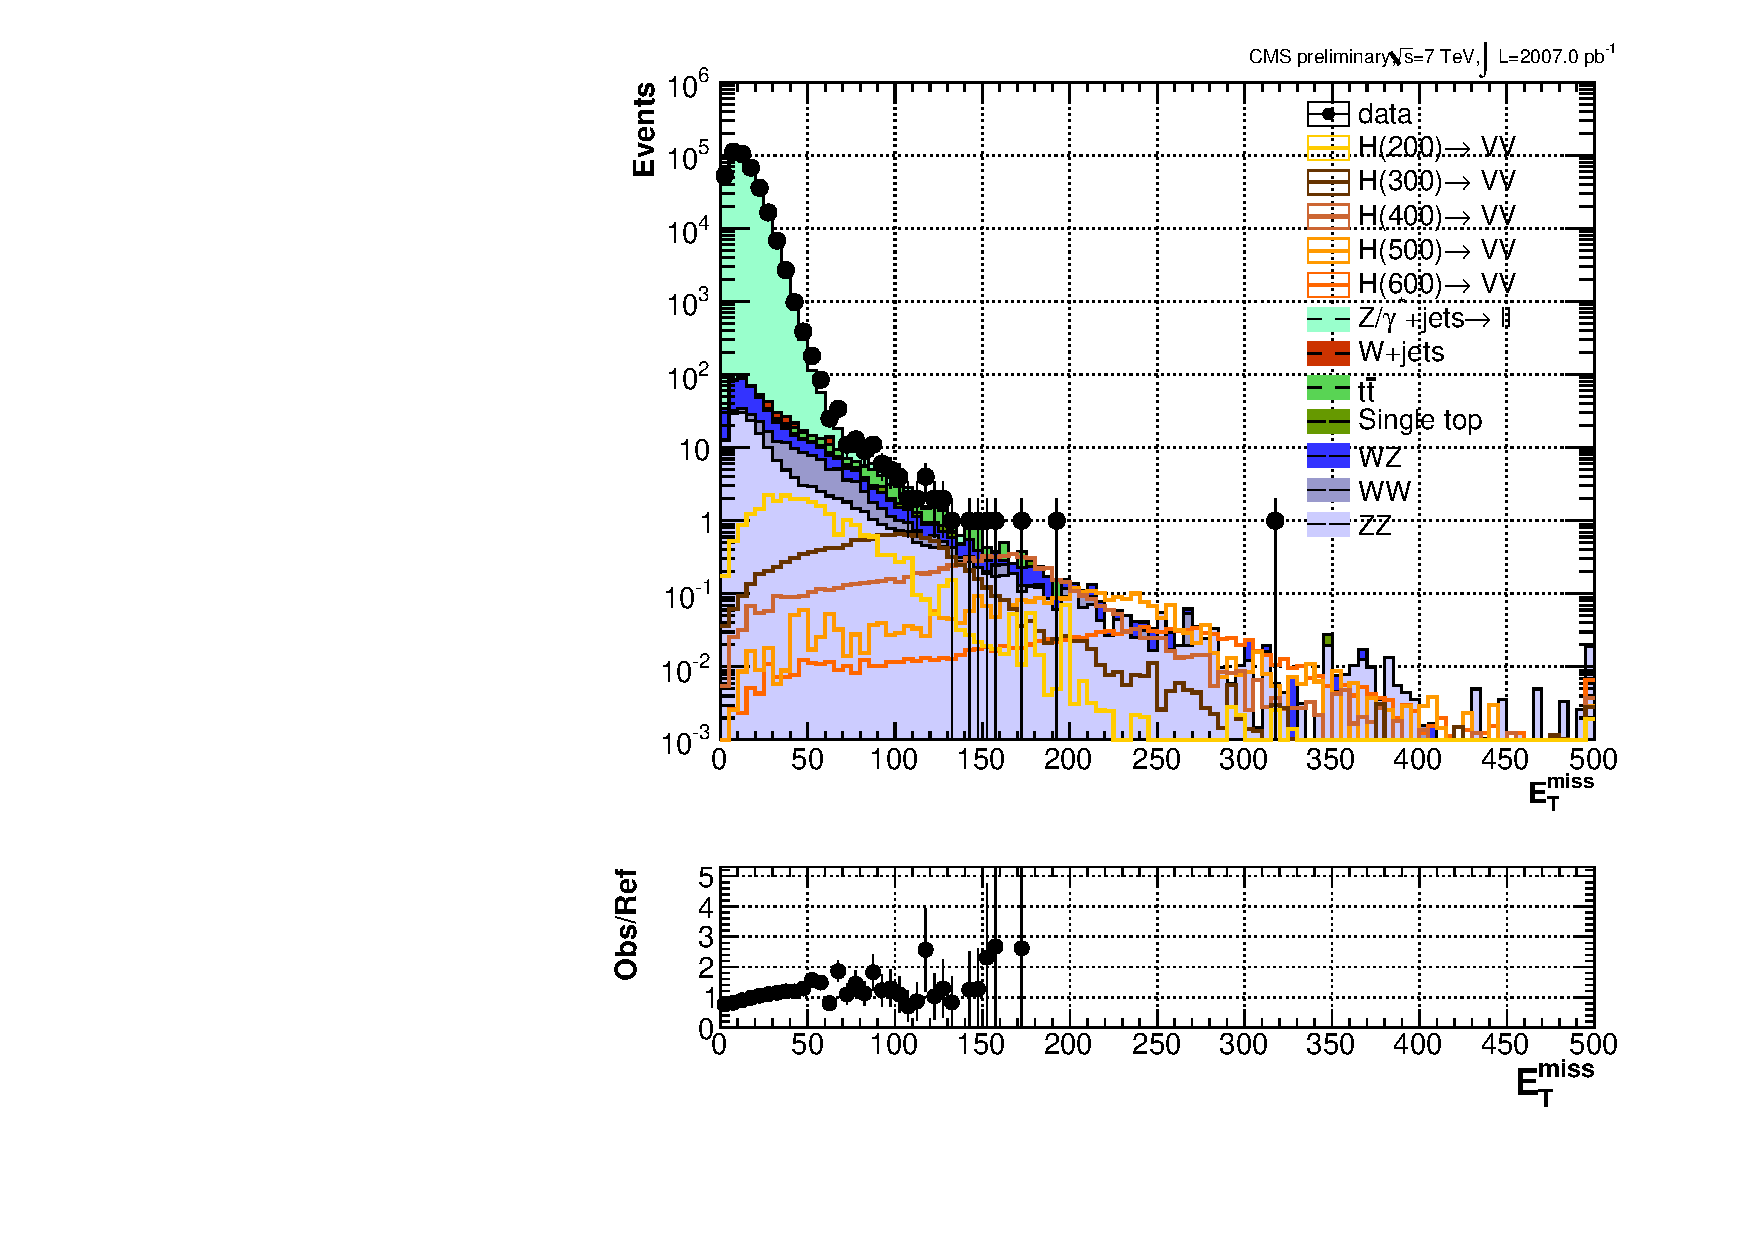
\includegraphics[width=0.46\textwidth]{img/ee_met}
\caption{\MET reconstructed in di-muon ({\em left}) and di-electron ({\em right}).}
\label{fig:metcontrol}
\end{center}
\end{figure}


\end{description}

In the next section the event yields after pre-selection of the sample and control plots are presented for the main variables of interest.


%%
%% EVENT YIELDS
%%
\subsection{Event yields after pre-seletion}
\label{subsec:eventyields}

The event yields after applying the pre-selection discussed in the previous section
are shown in Table~\ref{tab:presamplecutflow}.
An overall difference of $\approx$ 10\% is observed. An excess (deficit) of events is observed in the di-muon (di-electron) channel.

\begin{table}[htp]
\caption{Event yields for a total integrated luminosity of 1091~pb$^{-1}$. The uncertainties quoted are statistical only.}
\label{tab:presamplecutflow}
\begin{center}
\begin{tabular}{lccc} \hline\hline
Process                            & $|M-M_Z|<$15~GeV/c$^2$ & 3$^{rd}$-lepton veto & no b-tags\\ \hline
& & & \\\hline
\multicolumn{4}{c}{\bf $\mu\mu$ channel} \\\hline
H(200)$\rightarrow$ VV             & $ 29.3 \pm0.8 $    & $ 29.2 \pm0.8 $     & $ 26.7 \pm0.7 $  \\
H(300)$\rightarrow$ VV             & $ 13.72 \pm0.13 $  & $ 13.71 \pm0.13 $   & $ 12.44 \pm0.12 $\\
H(400)$\rightarrow$ VV             & $ 8.55 \pm0.08 $   & $ 8.54 \pm0.08 $    & $ 7.62 \pm0.07 $  \\
H(500)$\rightarrow$ VV             & $ 3.14 \pm0.11 $   & $ 3.14 \pm0.11 $    & $ 2.78 \pm0.10 $ \\
H(600)$\rightarrow$ VV             & $ 1.383 \pm0.018 $ & $ 1.380 \pm0.018 $  & $ 1.220 \pm0.017 $\\ \hline
ZZ                                 & $ 244.0 \pm1.0 $  & $ 234.5 \pm1.0 $     & $ 181.0 \pm0.9 $ \\
WW                                 & $ 87.8 \pm1.6 $   & $ 87.7 \pm1.6 $      & $ 84.9 \pm1.6 $  \\
WZ                                 & $ 330.5 \pm2.0 $  & $ 279.3 \pm1.8 $     & $ 26.2 \pm0.6 $  \\
Single top                         & $ 35.1 \pm1.1 $   & $ 34.4 \pm1.0 $      & $ 10.1 \pm0.6 $  \\
\ttbar                             & $ 396 \pm8 $      & $ 389 \pm8 $         & $ 41.8 \pm2.5 $  \\
W+jets                             & $ 0.30 \pm0.30 $  & $ 0.30 \pm0.30 $     & $ 0.30 \pm0.30 $ \\
$Z/\gamma^{*}+jets\rightarrow ll$  & $ ( 533.0 \pm0.4 ) \times10^{3} $  & $ ( 532.5 \pm0.4 ) \times10^{3} $  & $ ( 520.0 \pm0.4 ) \times10^{3} $ \\\hline
Total expected from SM             & $ ( 534.2 \pm0.4 ) \times10^{3} $  & $ ( 533.5 \pm0.4 ) \times10^{3} $  & $ ( 520.6 \pm0.4 ) \times10^{3} $ \\\hline
data                               & $ ( 605.3 \pm0.8 ) \times10^{3} $  & $ ( 604.4 \pm0.8 ) \times10^{3} $  & $ ( 588.3 \pm0.8 ) \times10^{3} $ \\\hline
& & & \\\hline
\multicolumn{4}{c}{\bf $ee$ channel} \\\hline
H(200)$\rightarrow$ VV             & $ 27.7 \pm0.8 $    & $ 27.7 \pm0.8 $     & $ 25.1 \pm0.7 $  \\
H(300)$\rightarrow$ VV             & $ 13.25 \pm0.13 $  & $ 13.23 \pm0.13 $   & $ 12.00 \pm0.12 $ \\
H(400)$\rightarrow$ VV             & $ 8.58 \pm0.08 $   & $ 8.56 \pm0.08 $    & $ 7.61 \pm0.07 $ \\
H(500)$\rightarrow$ VV             & $ 3.44 \pm0.11 $   & $ 3.43 \pm0.11 $    & $ 3.04 \pm0.10 $ \\
H(600)$\rightarrow$ VV             & $ 1.454 \pm0.015 $ & $ 1.452 \pm0.015 $  & $ 1.272 \pm0.015 $ \\ \hline
ZZ                                 & $ 228.3 \pm1.0 $   & $ 211.9 \pm0.9 $    & $ 163.1 \pm0.8 $  \\
WW                                 & $ 76.8 \pm1.5 $    & $ 76.7 \pm1.5 $     & $ 74.5 \pm1.5 $ \\
WZ                                 & $ 358.5 \pm2.1 $   & $ 303.6 \pm1.9 $    & $ 255.3 \pm1.8 $  \\
Single top                         & $ 35.0 \pm1.1 $    & $ 34.3 \pm1.0 $     & $ 10.5 \pm0.6 $   \\
\ttbar                             & $ 370 \pm7 $       & $ 363 \pm7 $        & $ 39.7 \pm2.4 $ \\
W+jets                             & $ 36 \pm7 $        & $ 36 \pm7 $         & $ 34 \pm7 $ \\
$Z/\gamma^{*}+jets\rightarrow ll$  & $ ( 465.03 \pm0.35 ) \times10^{3} $  & $ ( 464.51 \pm0.35 ) \times10^{3} $  & $ ( 453.10 \pm0.34 ) \times10^{3} $  \\\hline
Total expected                     & $ ( 466.13 \pm0.35 ) \times10^{3} $  & $ ( 465.54 \pm0.35 ) \times10^{3} $  & $ ( 453.67 \pm0.34 ) \times10^{3} $  \\\hline
data                               & $ ( 413.8 \pm0.6 ) \times10^{3} $    & $ ( 413.2 \pm0.6 ) \times10^{3} $    & $ ( 401.9 \pm0.6 ) \times10^{3} $    \\\hline\hline
\end{tabular}
\end{center}
\end{table}

%%
%%
%%
\section{Verification of the reconstructed missing transverse energy}
\label{sec:met}

The following section we discuss different strategies adopted in the choice of the variable used to reduce the contamination
from the instrumental background, i.e., from processes in which the \MET is mismeasured.
The main sources of mis-measurement of this quantity are the underestimate of the hadronic recoil
of $Z$ bosons, due to jet energy scale and resolution as well as detector acceptance,
and the contamination from pileup.
In the first part we describe a variable developed with the purpose of reducing the error in the estimate of the hadronic recoil of the $Z$ bosons.
The performance of this variable is compared with standard \MET among others.
In the second part we describe the strategies developed to verify the contamination from pileup events with high hadronic activity.

%%%
%%% REDUCED MET
%%%
\subsection{Description of the reduced \MET method}
\label{subsec:redmet}

We adopt the definition of reduced missing transverse energy (\RMET) for our analysis.
The definiton is an upgrade of the original concept developed by the D0 collaboration~\cite{Abazov:2008yf}.
In this method the recoil of the dilepton is decomposed using either the dilepton:

\begin{itemize}
\item direction, in case the two leptons are collimated, i.e. $\Delta\phi^{ll}<\pi/2$;
\item bisector, in case the two leptons are reconstructed with an open angle, i.e.   $\Delta\phi^{ll}>\pi/2$;
\end{itemize}

In the case of two leptons reconstructed with an open angle 
the bisector of the dilepton is defined transversely to the axis which maximizes the dilepton transverse momentum,  i.e. the thrust axis($\vec{t}$):

\begin{equation}
\vec{t} =\frac{1}{|\vec{l}_1-\vec{l}_2|}(\vec{l}_1 - \vec{l}_{2})
\label{eq:thrust} 
\end{equation}

where $l_1$ ($l_2$) is the 3-momentum of the leading (trailer) lepton. 
We adopt the convention to define the bisector ($\vec{b}$) as pointing in the same direction as the leading lepton, i.e.:

\begin{equation}
\vec{b}\cdot\vec{t}=0 ~~~\wedge~~~ \vec{b}\cdot\vec{l}_1>0
\label{eq:bisector} 
\end{equation}

The thrust and bisector are used to define the projections of the dilepton recoil which can be estimated from two sources:

\begin{itemize}
\item clustered recoil ($\vec{R}^{\text{clust}}$), from the jets reconstructed in the event;
\item unclustered recoil ($\vec{R}^{\text{uncl}}$), from the sum of all particle flow candidates with the exception of the two leptons;
\end{itemize}

Originally the \RMET variable is computed with the following prescriptions:

\begin{enumerate}
\item the jets which contribute to each component of $\vec{R}^{\text{clust}}$ have to be found in the opposite direction with respect to the correspondent dilepton projection  
\item likewise the projections of the unclustered recoil are considered to be 0 if pointing in the same direction as the correspondent dilepton projection
\item the estimate of the recoil along each direction is made conservatively by taking the minimum of the two estimate, i.e. $R_i = \min \{ R_i^{\text{clust}},R_i^{\text{uncl}} \}$ 
\end{enumerate}

In this study we argue that 1. and 2. should not be used as they lead to an incomplete description of the recoil of the dilepton system for both instrumental background
(i.e. $Z$ events) and signal events.
In the first case the prescription to use jets which point in the opposite direction of the dilepton is compromised by the ocurrence of jet production
in the underlying event or even by multiple interaction. If only a subset of the jets is accounted for this leads inevitably to a wrong estimate of the true recoil.
In the second case we argue that highly boosted Higgs will be measured with the two Z's in the same hemisphere and therefore both the dilepton and the \MET will be pointing in the same direction
and found to be recoiling against a jet system. For these topologies the recoil will be estimated as being 0, leading to a consequent inefficiency of identifying the signal at high values of \RMET.
Instead we define \RMET from the minimum imbalance found using either the clustered or the unclustered recoil of the system.
Each component of \RMET is computed and minimized individually as

\begin{equation}
{\rm red-}\cancel{E}_{T_i}^{k} =\vec{p}_{T}^{ll}\cdot \vec{i} + \alpha R^{\text{k}}_{i}
\label{eq:rmet}
\end{equation}

where k=clustered/unclustered and $\alpha$ is a scale factor which we consider always to be 1.
The absolute \RMET measurement is taken from the quadratic sum of the two components.
The procedure just described assumes a conservative scenario for jet energy and unclustered \MET reconstruction and resolution.
It is also expected to be effective against pileup events as jets are seeded using particle flow candidates associated to the primary vertex selected for each event. 
Our definition of \RMET is compared with the original one from D0 in Fig.~\ref{fig:redmet} for di-muon events.
It can be seen that the D0 definition yields a distribution with a very good resolution but which artificially 
accumulates events with \RMET=0 even for the signal. This result is strictly related to the topology of the boosted Higgs events
and can be mostly identified from events with 1 or 2 jets.
It can also be observed a better agreement between data and \MC for the definition of \RMET adopted by us.

\begin{figure}[htp]
\begin{center}
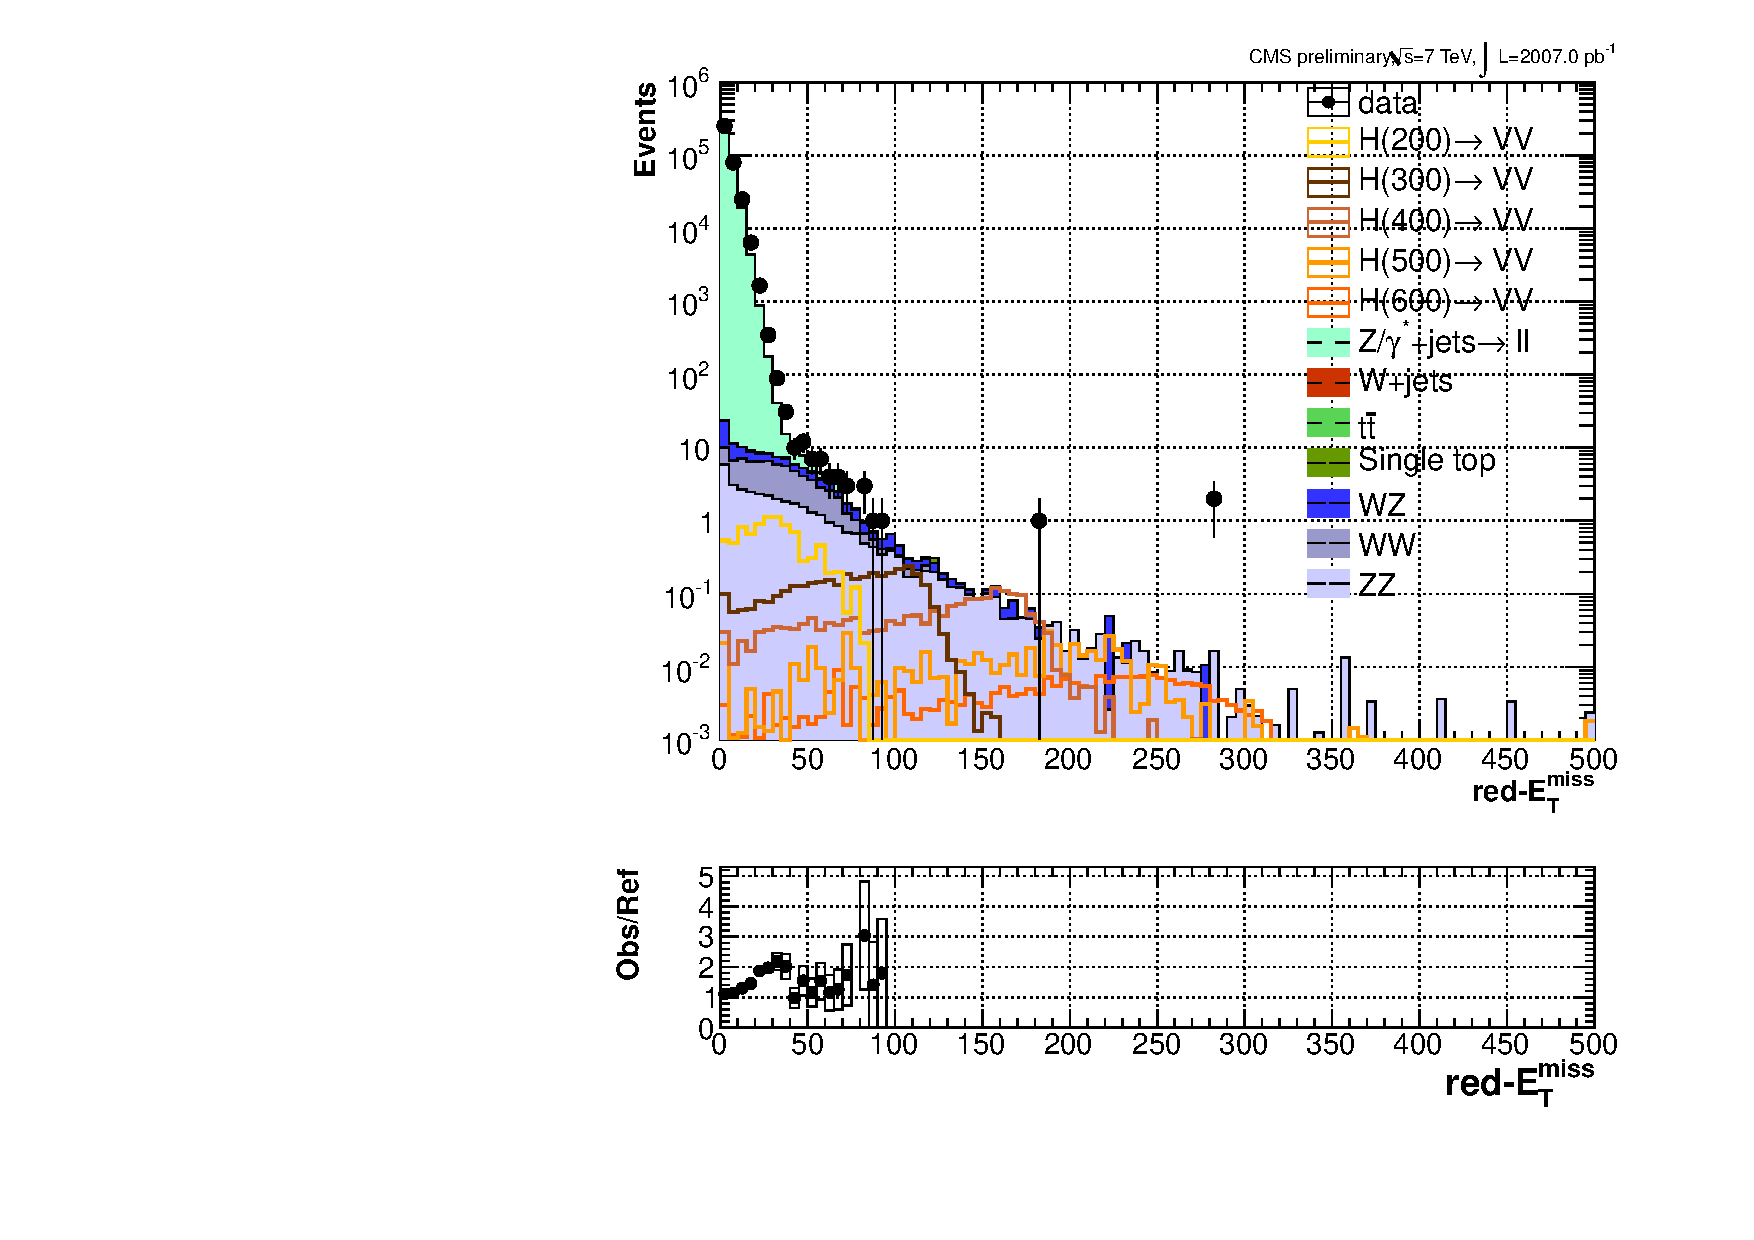
\includegraphics[width=0.32\textwidth]{img/mumueq0jets_redMet_d0}
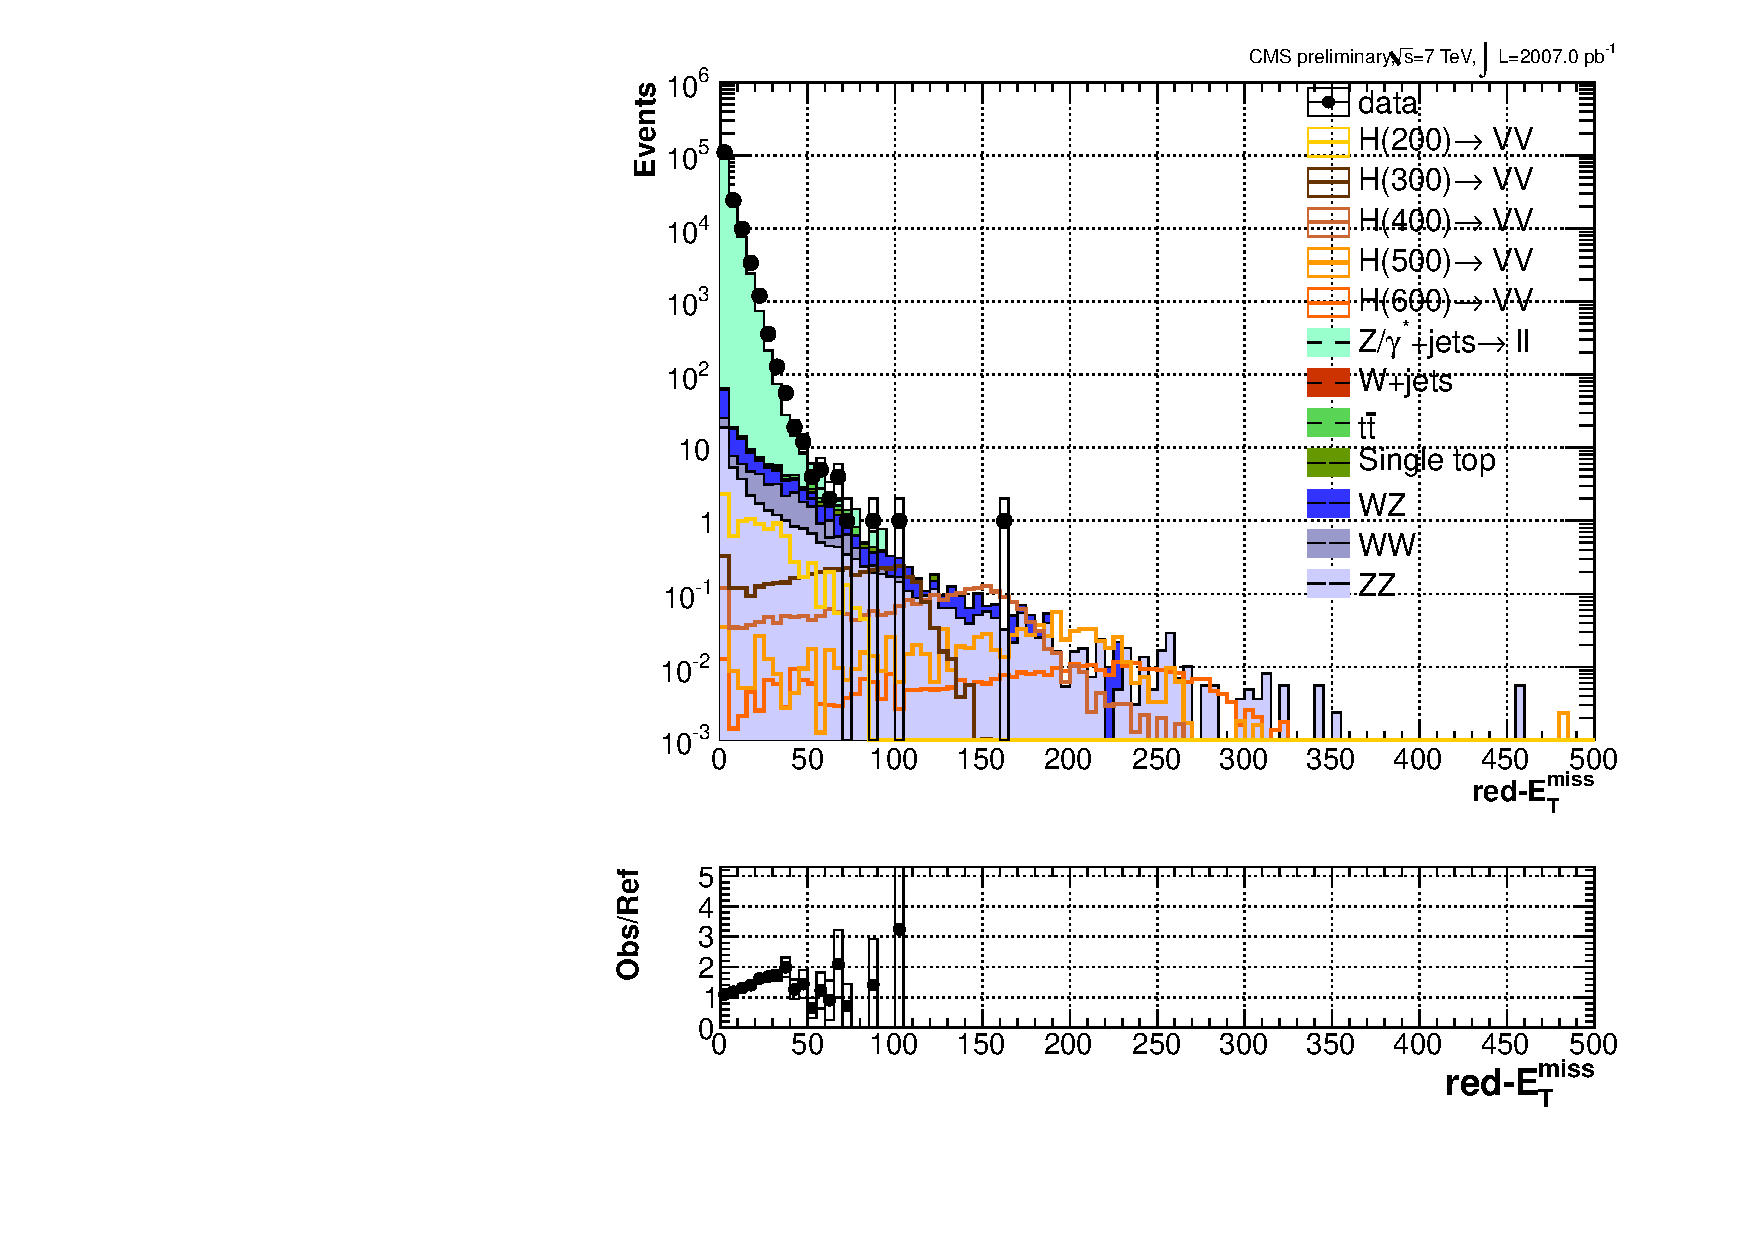
\includegraphics[width=0.32\textwidth]{img/mumueq1jets_redMet_d0}
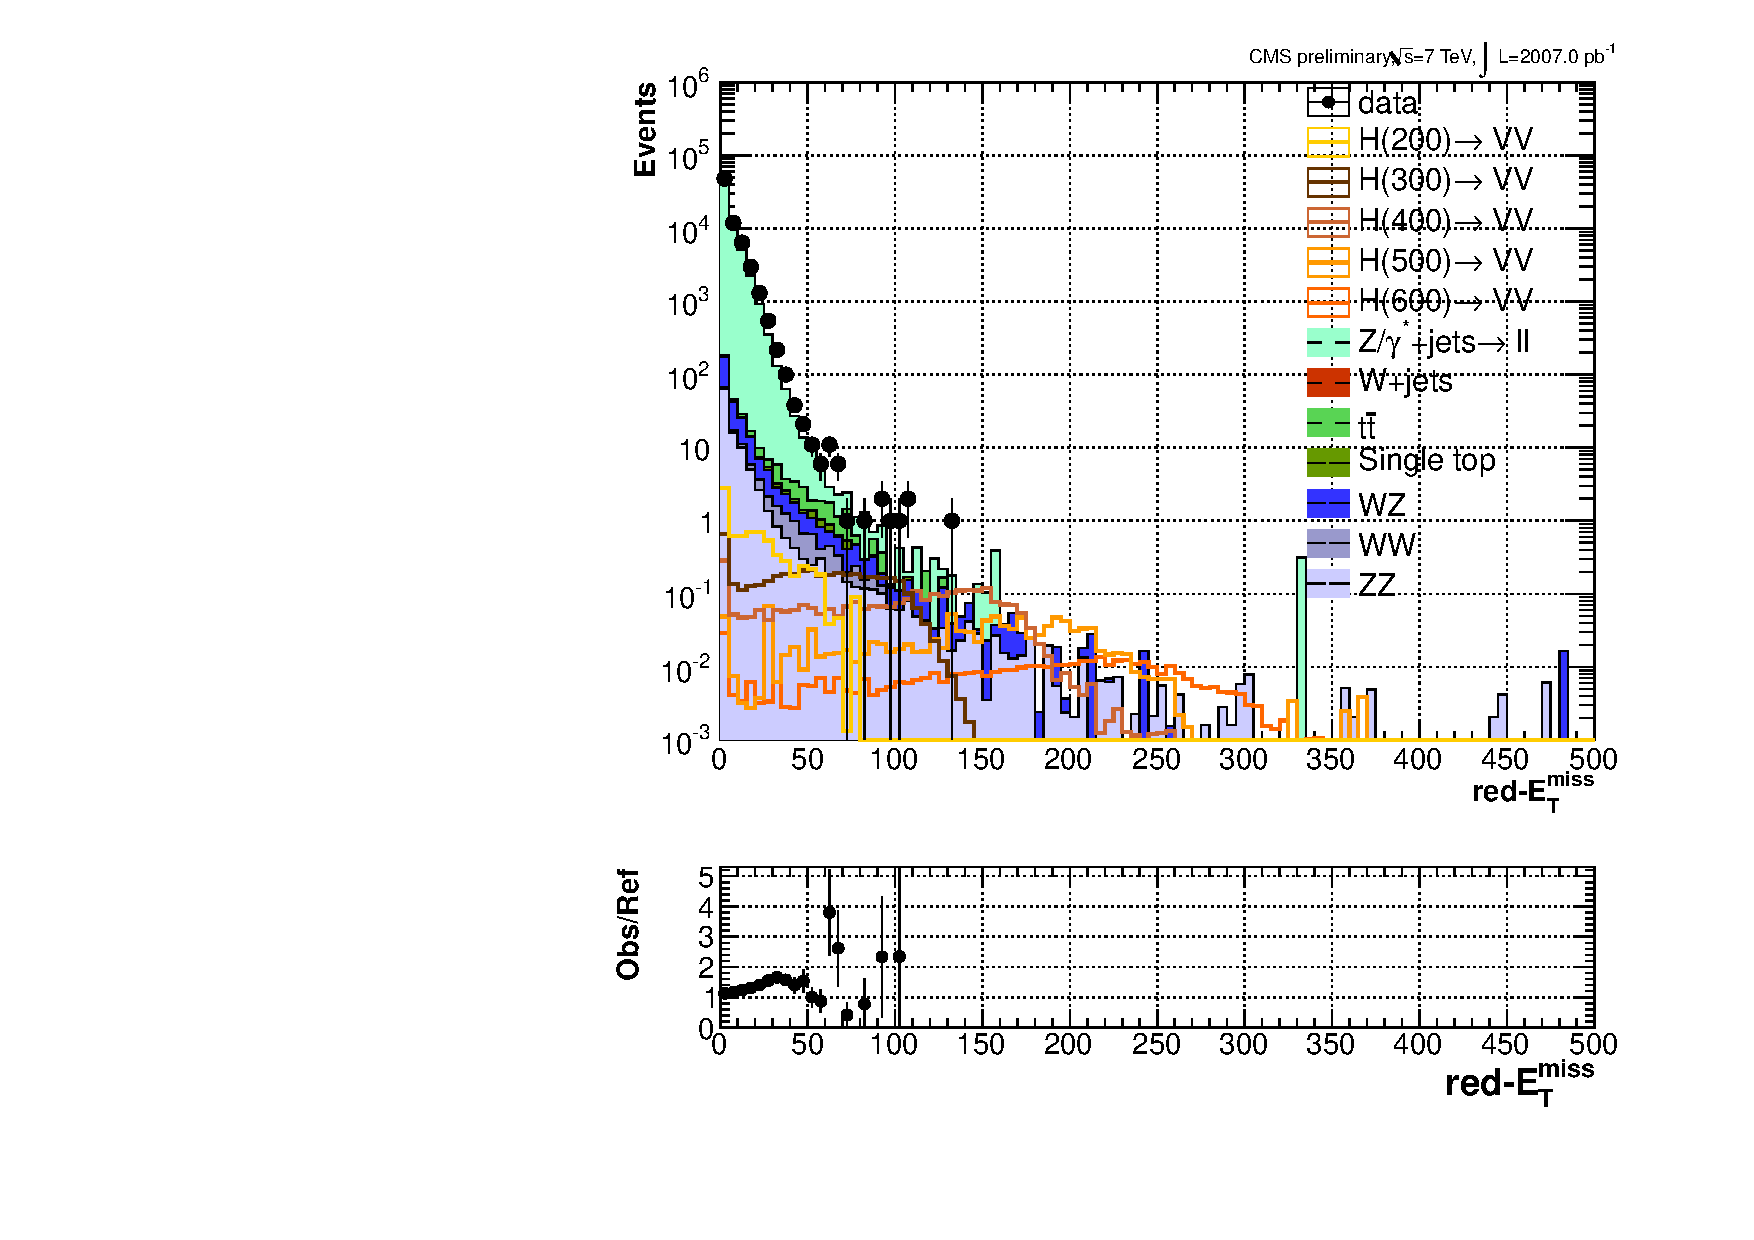
\includegraphics[width=0.32\textwidth]{img/mumugeq2jets_redMet_d0}\\
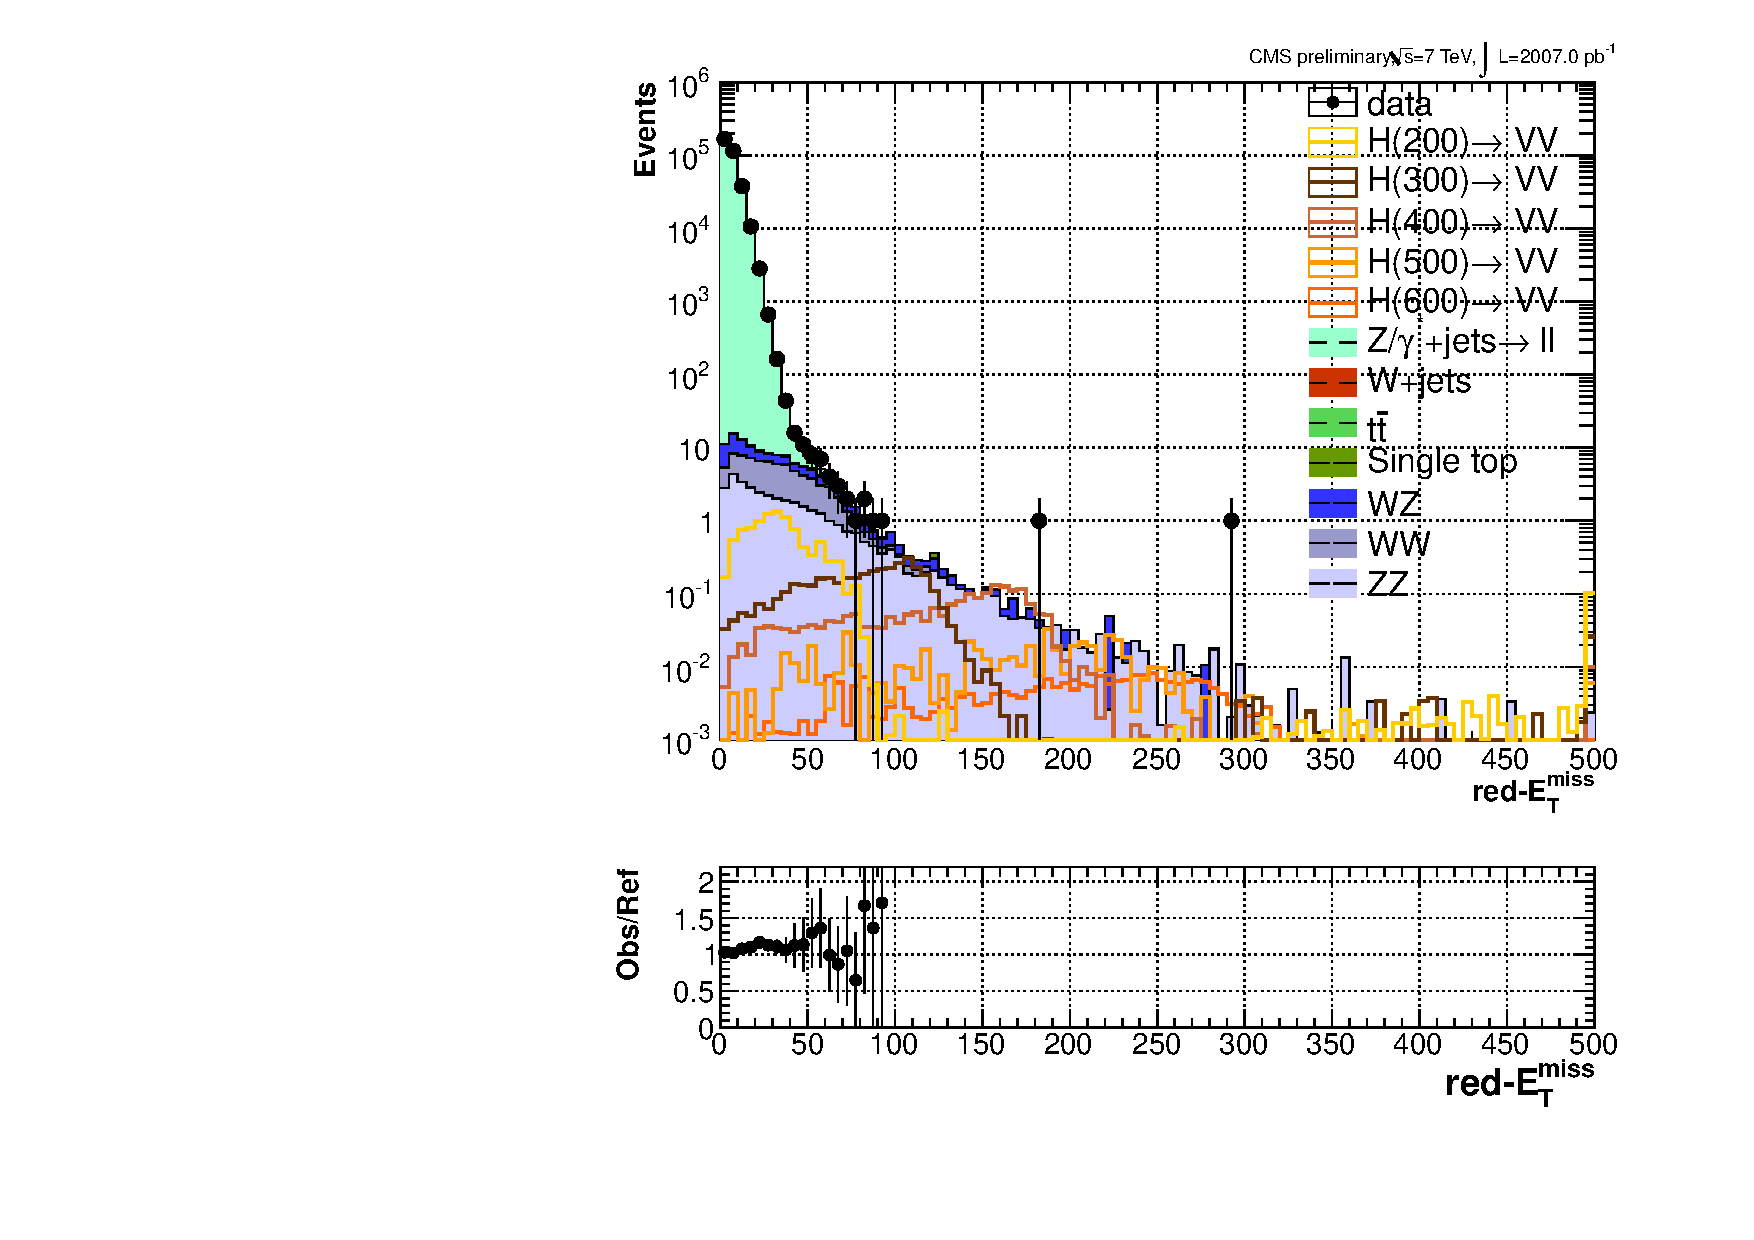
\includegraphics[width=0.32\textwidth]{img/mumueq0jets_redMet}
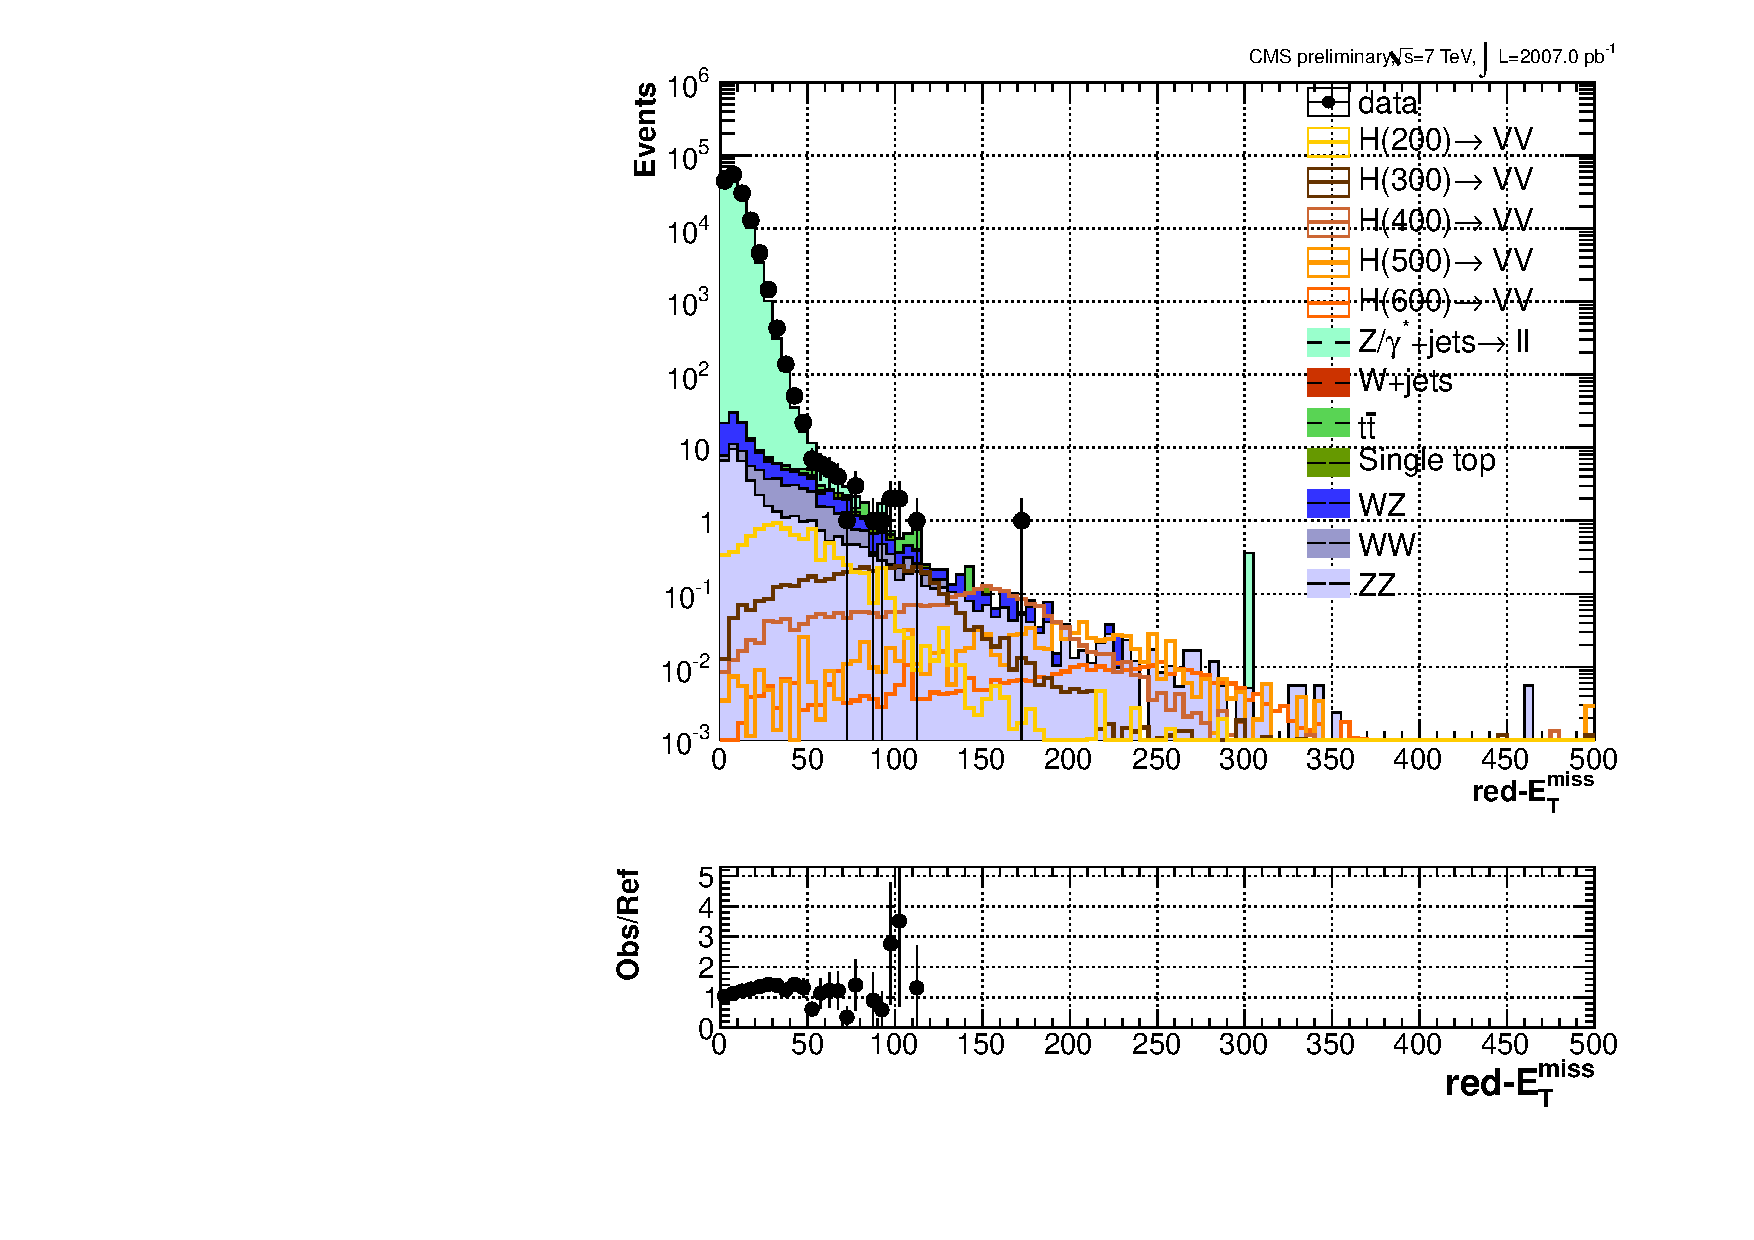
\includegraphics[width=0.32\textwidth]{img/mumueq1jets_redMet}
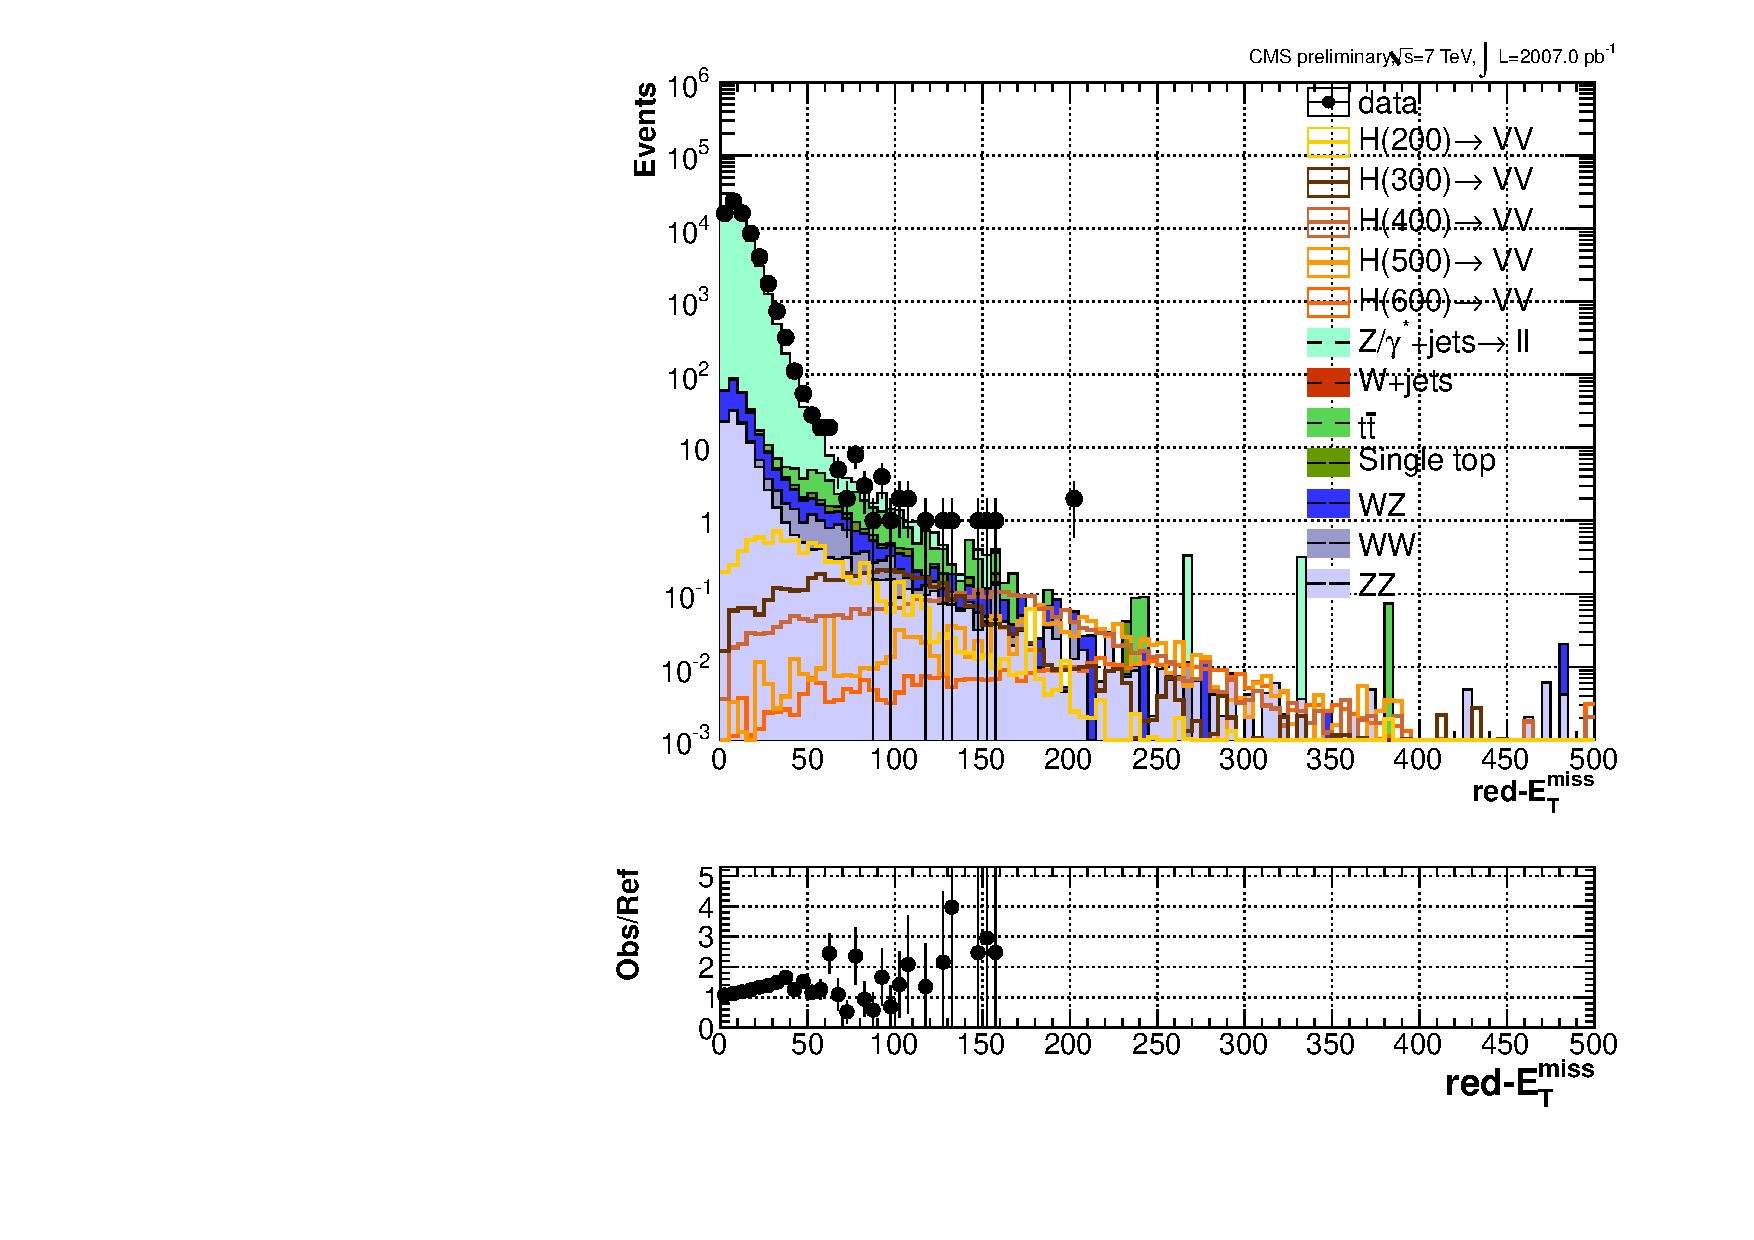
\includegraphics[width=0.32\textwidth]{img/mumugeq2jets_redMet}
\caption{\RMET distribution in di-muon events with 0 ({\em left}), 1 ({\em center}) or 2 ({\em right}) jets.
The original definition from the D0 collaboration is shown on top to be compared with the definition adopted in this manuscript shown on bottom.}
\label{fig:redmet}
\end{center}
\end{figure}

The \RMET variable is adopted in the event selection for the Higgs boson and
two working points (medium and tight) are defined in order to reject the instrumental background ($Z$ events) at a 10$^3$ and 10$^4$ rate level.
The medium (tight) working point is used as a base selection for medium (high) mass search corresponding to 200-300 ($>$300) GeV/c$^2$.
The working points are defined independently for each jet multiplicity bin in order to maximize the rejection power of the instrumental background
\footnote{The working points are obtained from a parameterization of the efficiency curves where the efficiency
is defined from the fraction of events of a given process observed above a given threshold.
The parametrization used is a 2$^{nd}$ order polynomial function of the logarithm of the \RMET cut.}.
Table~\ref{tab:redmetwp} summarizes the values adopted for the medium and tight \RMET working points.

\begin{table}[htp]
\caption{Working points for different Drell-Yan rejection powers for \RMET.
The expected efficiency for the selection of different Higgs masses is shown for reference.}
\label{tab:redmetwp}
\begin{center}
\begin{tabular}{lccc} \hline\hline
Jet multiplicity      & =0 jets & =1 jets & $\geq$ 2 jets  \\\hline
                      &         &         & \\\hline
\multicolumn{4}{c}{{\bf Medium working point} ($10^{-3}$ rejection factor)} \\\hline
Cut value             & 30.5    & 38.8    &  50.8\\
$\varepsilon$(200)    & 59.7\%  & 52.5\%  &  41.6\% \\
$\varepsilon$(300)    & 91.2\%  & 88.5\%  &  81.1\% \\
$\varepsilon$(400)    & 94.8\%  & 93.2\%  &  90.2\% \\\hline
                      &         &         & \\\hline
\multicolumn{4}{c}{{\bf Tight working point} ($10^{-4}$ rejection factor)} \\\hline
Cut value             & 39.0    & 52.4    &  78.7\\
$\varepsilon$(200)    & 38.9\%  & 32.3\%  &  17.8\%\\
$\varepsilon$(300)    & 87.6\%  & 79.5\%  &  53.1\%\\
$\varepsilon$(400)    & 91.2\%  & 89.1\%  &  81.3\% \\\hline\hline
\end{tabular}
\end{center}
\end{table}

The performance of the \RMET can be further quantified relatively to the standard \MET measurement 
as well as other \MET related variables. The \MET measurement can be made more robust against pileup contamination
by considering the minimum of two transverse momenta sums: of all particle flow candidates (\MET) or of all 
charged particle flow candidates which can be associated to the primary vertex of the event (\tkMET).
This variable was introduced in Section~\ref{subsec:trigrec} to characterize the properties of the primary vertex.
As it is built using a vertex constraint it is expected to have a small contamination from pileup.
It's resolution is however degraded and has a non trivial dependence on the topology of the event,
therefore the minimum is taken with respect to the full \MET measurement.
A third variable which is worth comparing to is the projected missing transverse energy (\projMET)
which aims at minimizing the poor reconstruction of leptons.
Even if this is not considered to be the main problem affecting the \MET measurement under the $Z$ boson peak
we compare its performance with the other measurements.
This variable is computed as the transverse component of \MET 
relatively to the closest lepton (if closer than $\pi/2$ in the azimuthal angle)
or the full \MET otherwise
\footnote{\projMET can be explicitly written from the following formulas.
Let $\delta\phi^{\rm min}=\min\{\delta\phi(E_{T}^{miss},l^1),\delta\phi(E_{T}^{miss},l^2)\}$
be the azimuthal angle between the \MET vector and the transverse momentum of the closest lepton.
Then \projMET=\MET$\cdot\sin\delta\phi^{\rm min}$ if $\delta\phi^{\rm min}<\pi/2$ or \MET, otherwise.}.
Following the prescription adopted by~\cite{CMS-PAS-HIG-11-003}
the dependency on pile-up is reduced by taking the minimum \projMET computed from \MET and \tkMET.
This minimization exploits further the correlation between both estimates in signal and 
uncorrelation otherwise, as in Drell-Yan events.
Fig.~\ref{fig:metperformances} summarize the performance of each variable 
for the rejection of the instrumental background considering two hypothetical higgs boson masses.
The performance is compared for events selected under the $Z$ boson peak and in the side-band region, i.e.
dilepton events with a mass compreehended in the 61-76 and 106-121 GeV/c$^2$ range.
It is visible that the \RMET approach is performing better overall in the $Z$ boson peak region which is the region of interest for our study.
The performance of the \RMET variable is significantly better in the low mass regime under the $Z$ mass peak.

\begin{figure}[htp]
\begin{center}
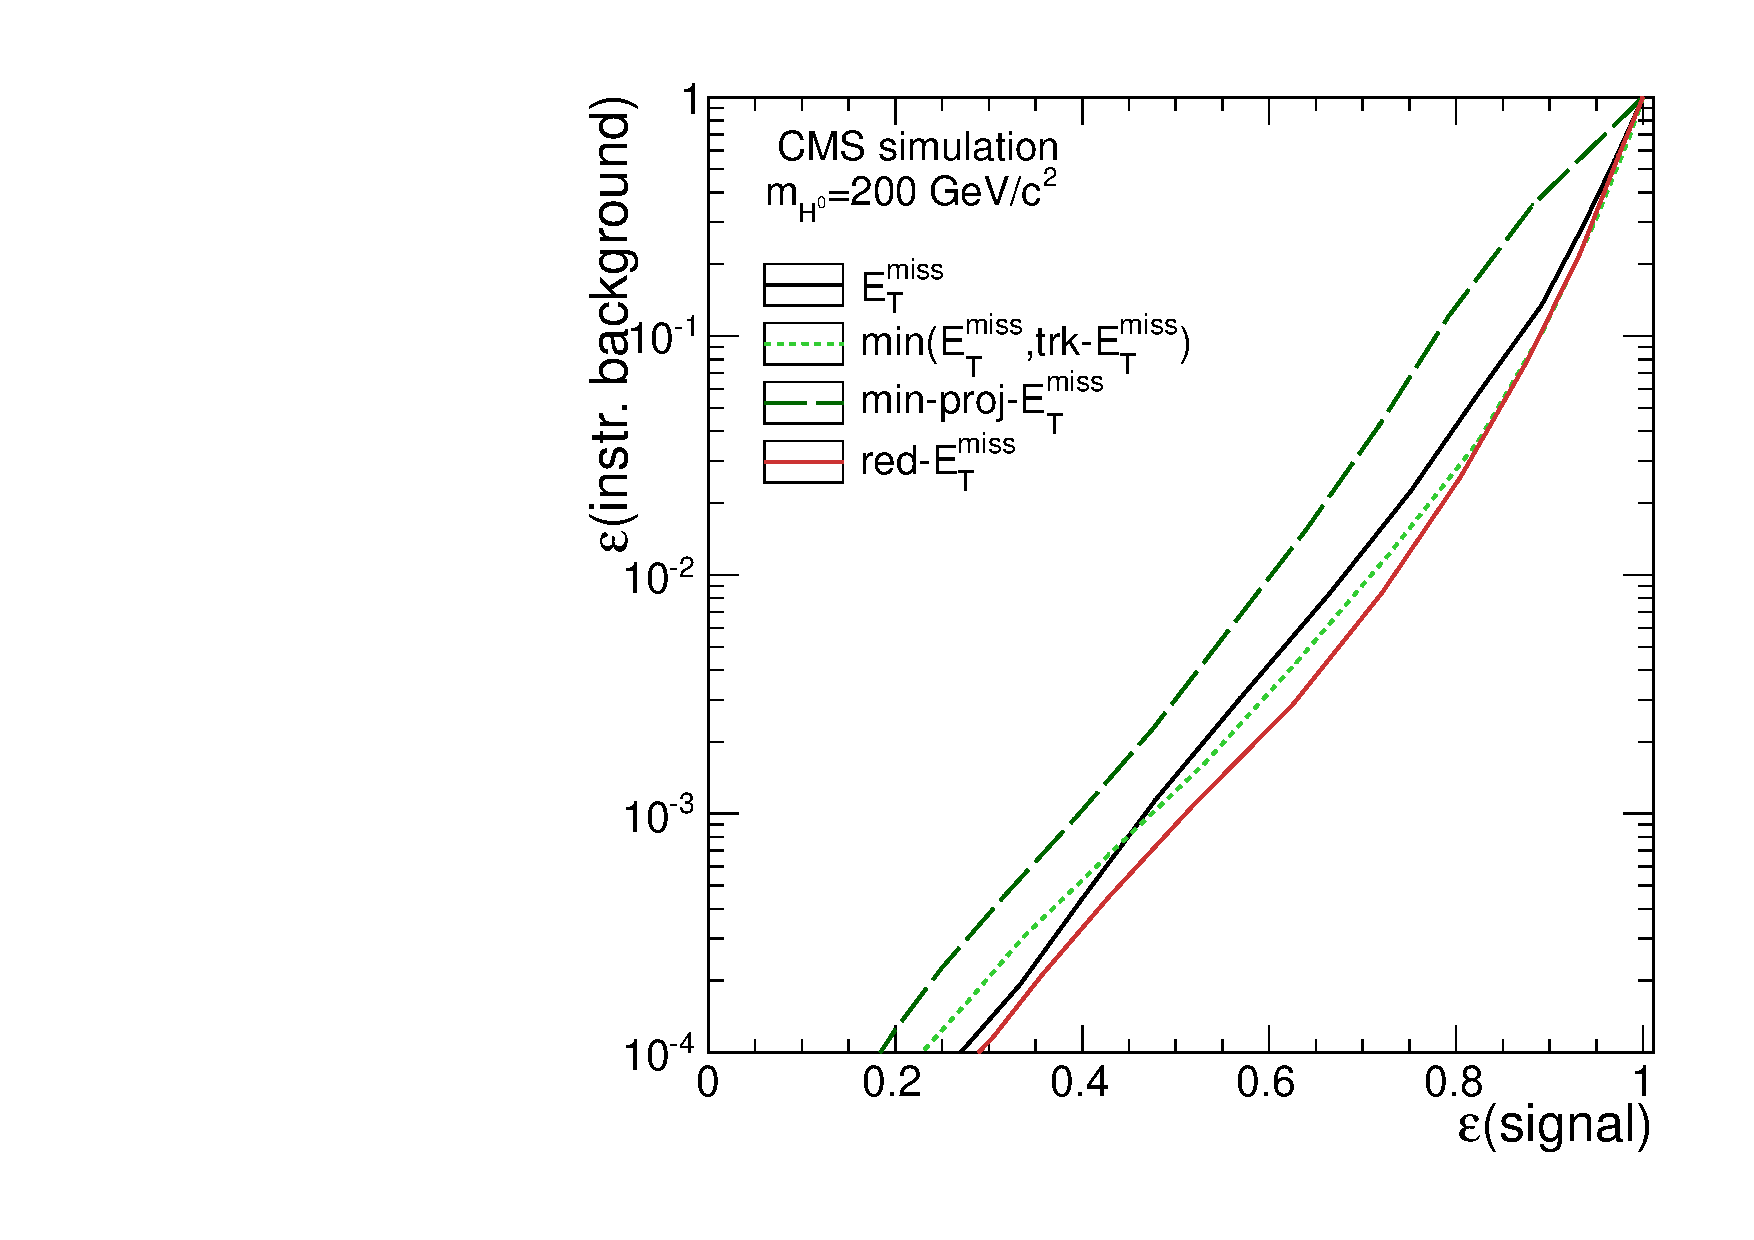
\includegraphics[width=0.4\textwidth]{img/eff200}
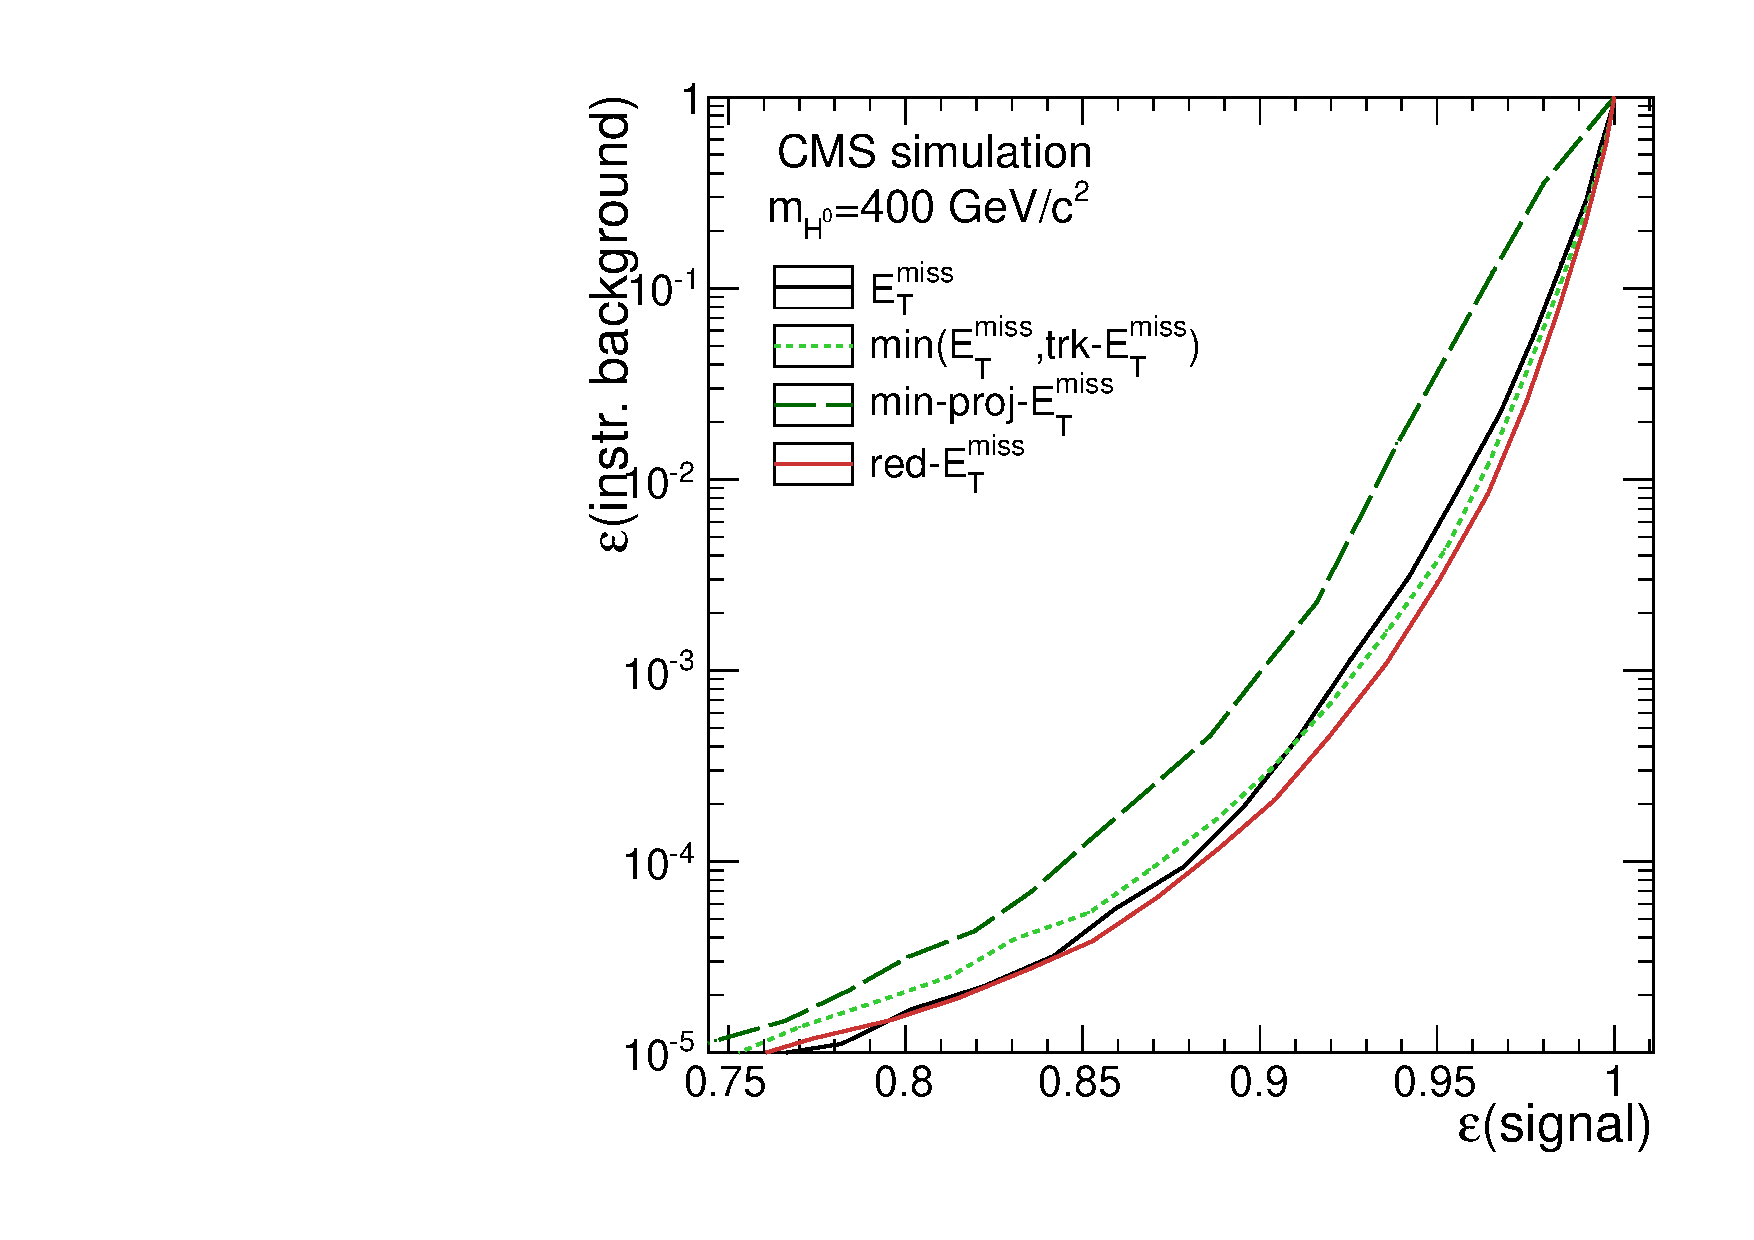
\includegraphics[width=0.4\textwidth]{img/eff400}\\
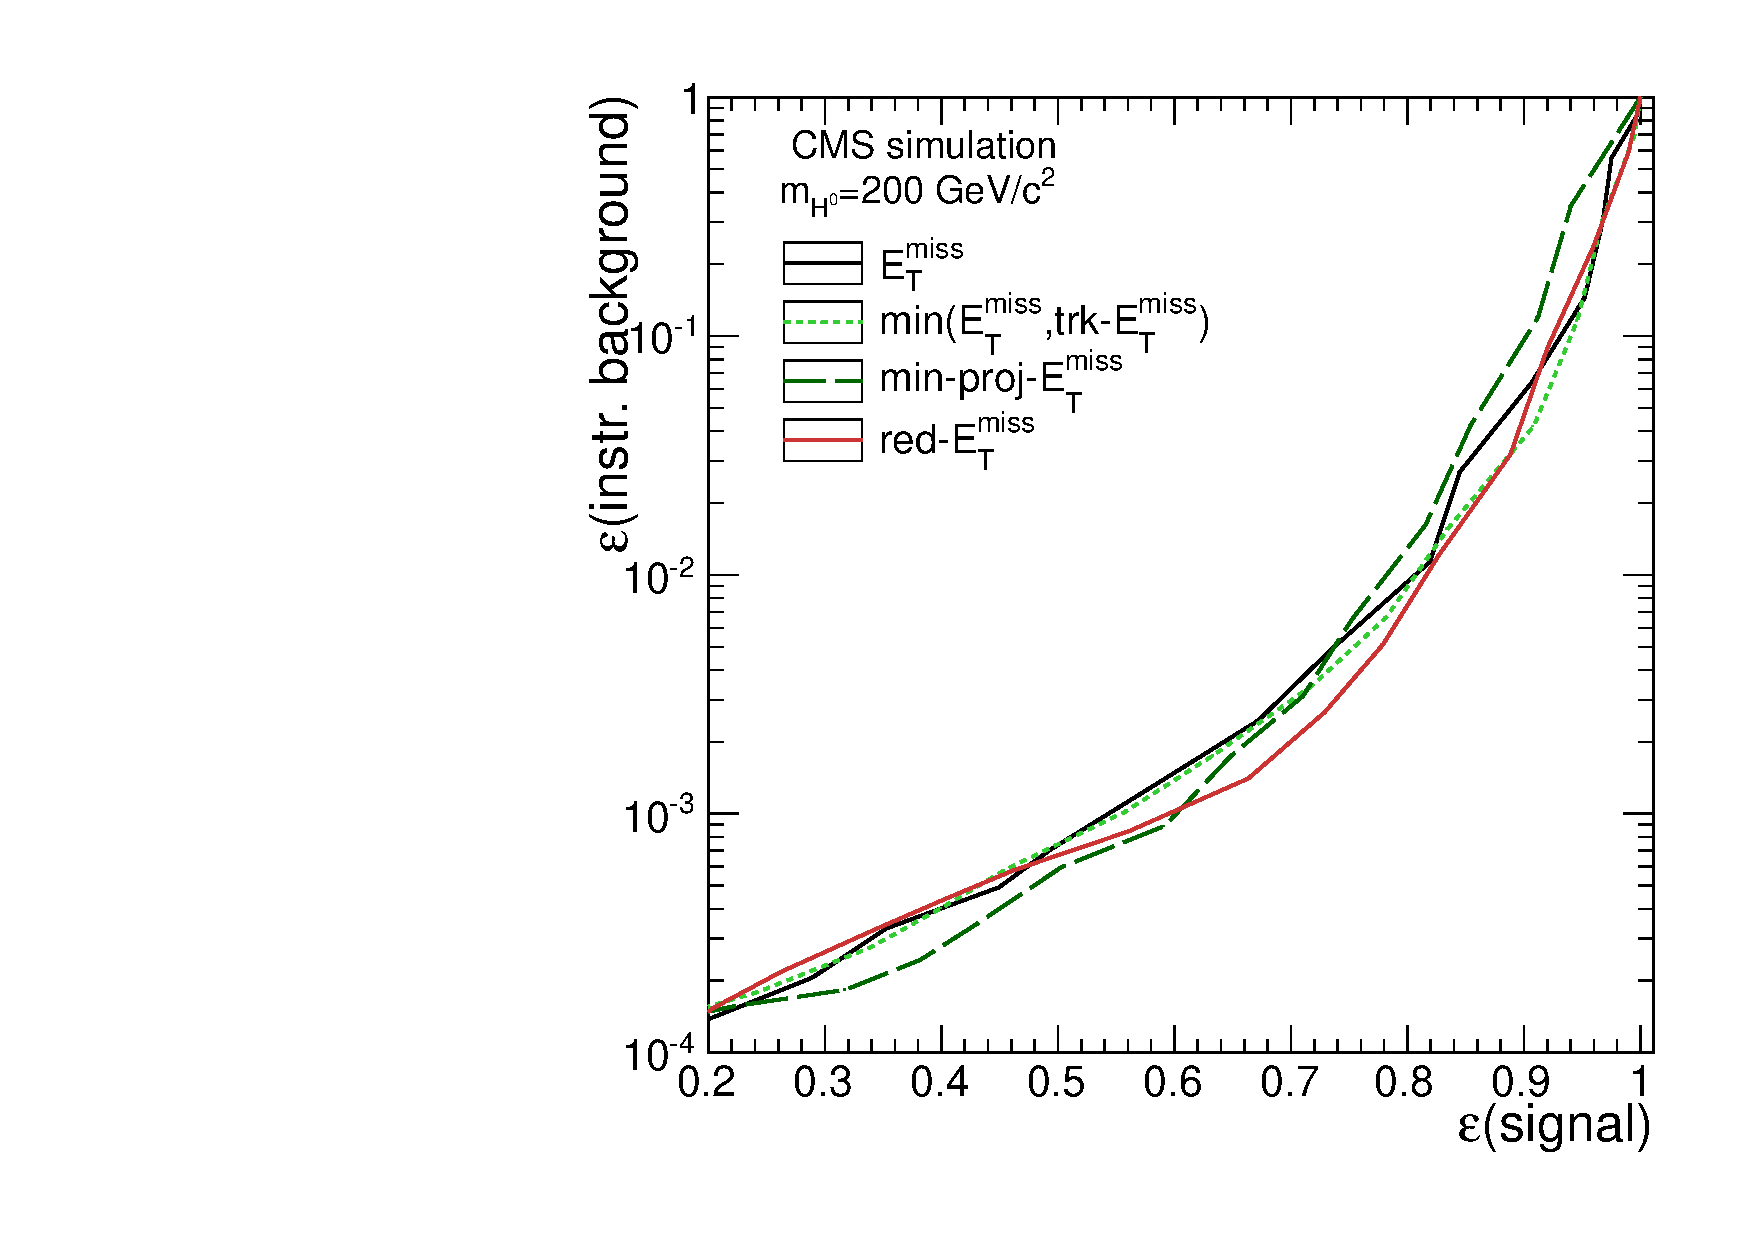
\includegraphics[width=0.4\textwidth]{img/eff200_zsideband}
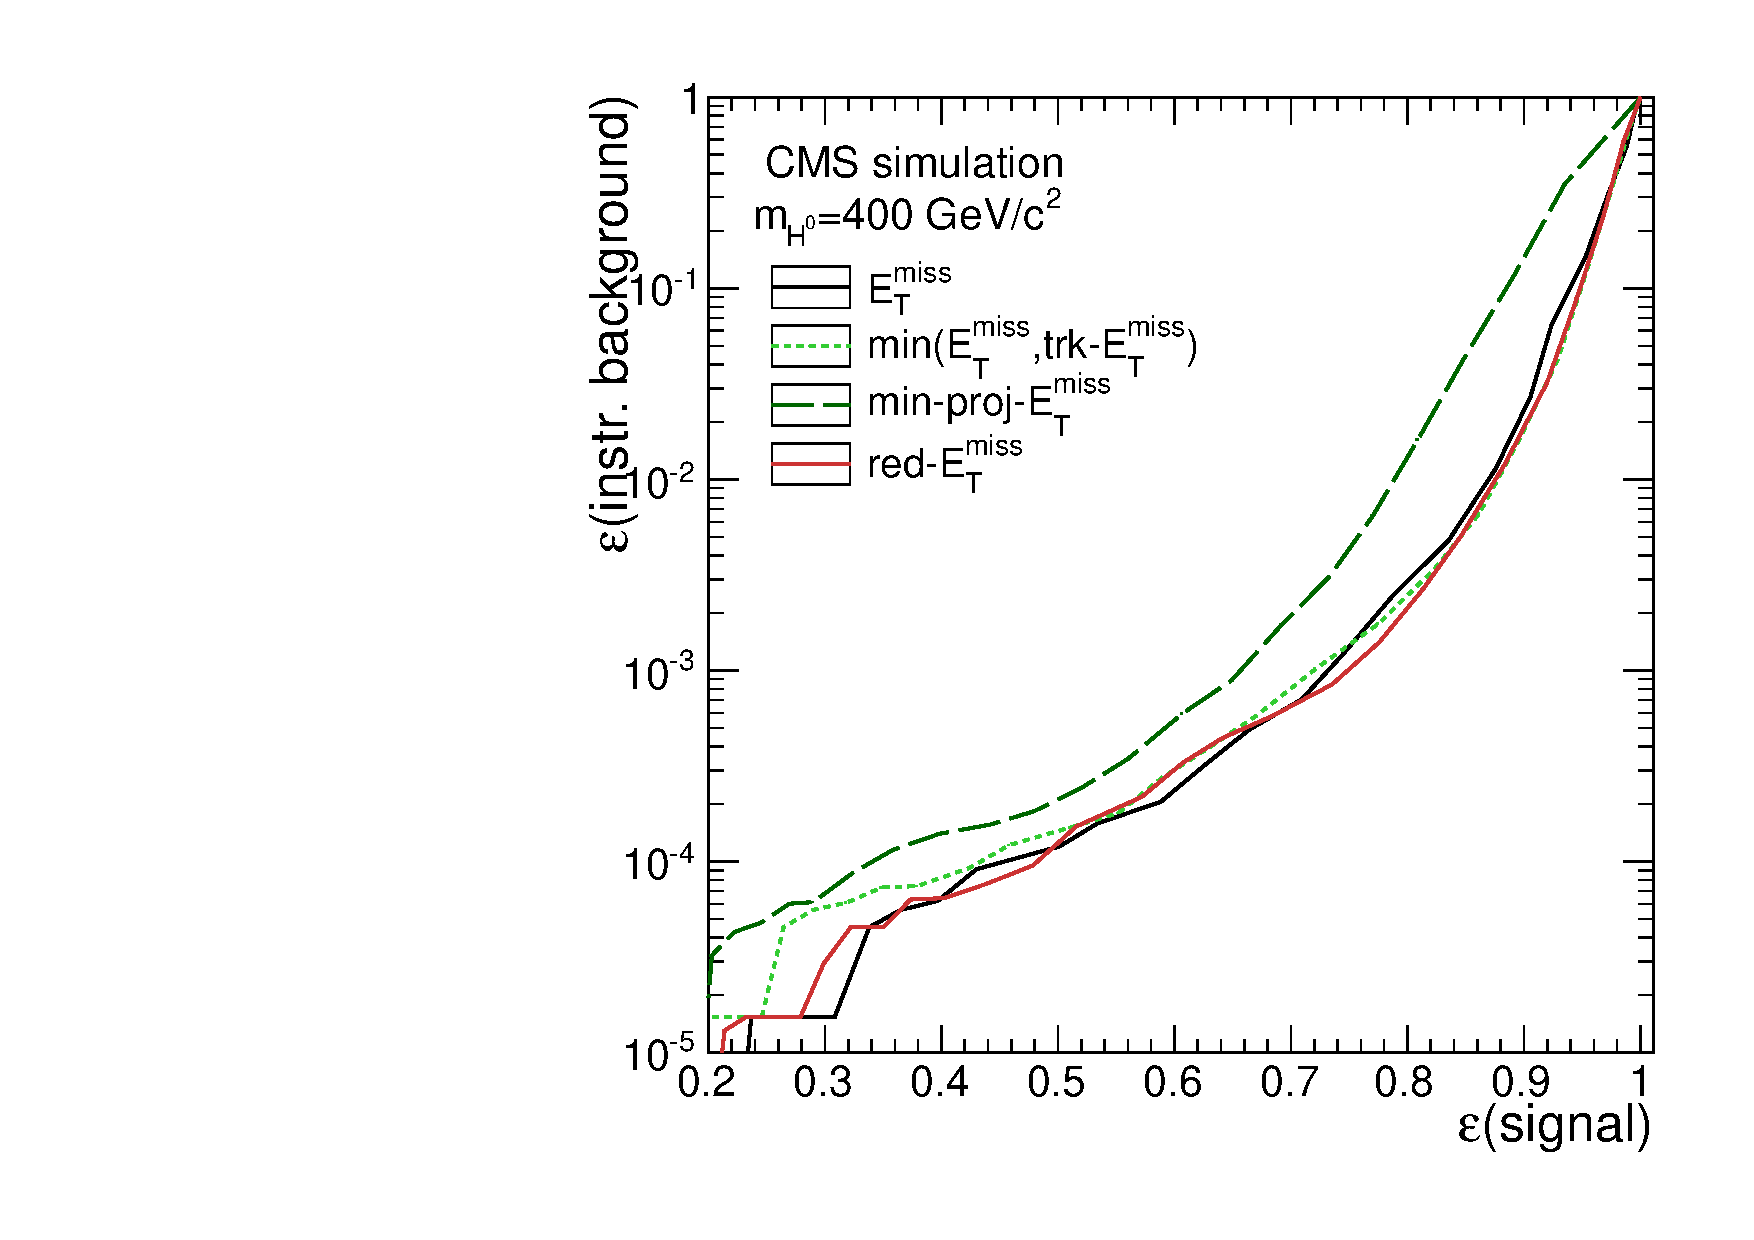
\includegraphics[width=0.4\textwidth]{img/eff400_zsideband}
\caption{Efficiency curves for signal versus instrumental background acceptance for different \MET variables.
Signal is considered as a 200~GeV/c$^2$ ({\em left}) or a 400~GeV/c$^2$ ({\em right}) Higgs boson.
The {\em top} plots show the results obtained in the Z-boson mass region while the {\em bottom} plots show the results obtained in the side-band region.}
\label{fig:metperformances}
\end{center}
\end{figure}

The performances can be further compared in terms of robustness against the variation of the pileup scenario.
This test is summarized in Fig~\ref{fig:metperformancevspileup}. 
We conclude that all approaches have a dependency on the pileup scenario which is minimized when taking
the \tkMET or \RMET approaches. The dependency for these pseudo-\MET variables is observed to be approximately linear
in both the average and RMS of the spectrum.

\begin{figure}[htp]
\begin{center}
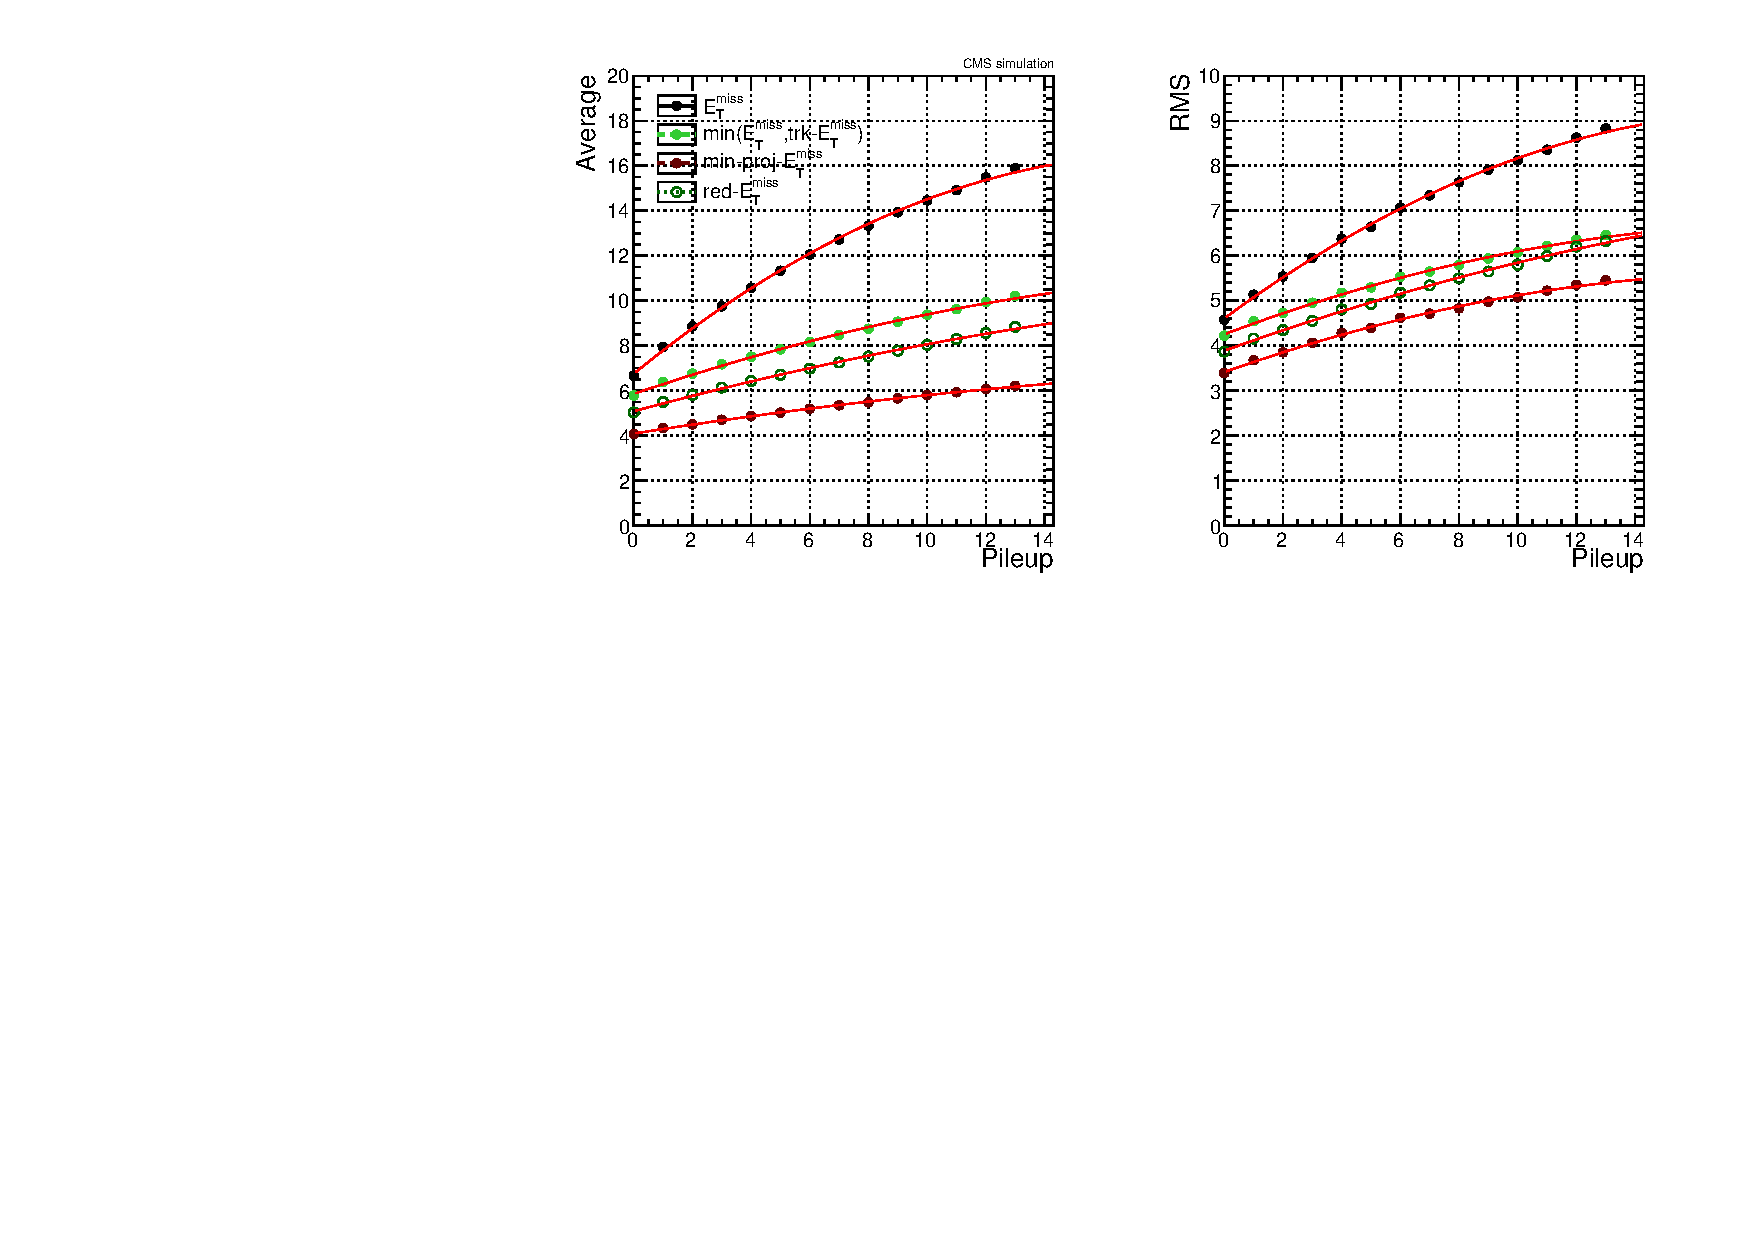
\includegraphics[width=0.9\textwidth]{img/metvariablesVsPileup}\\
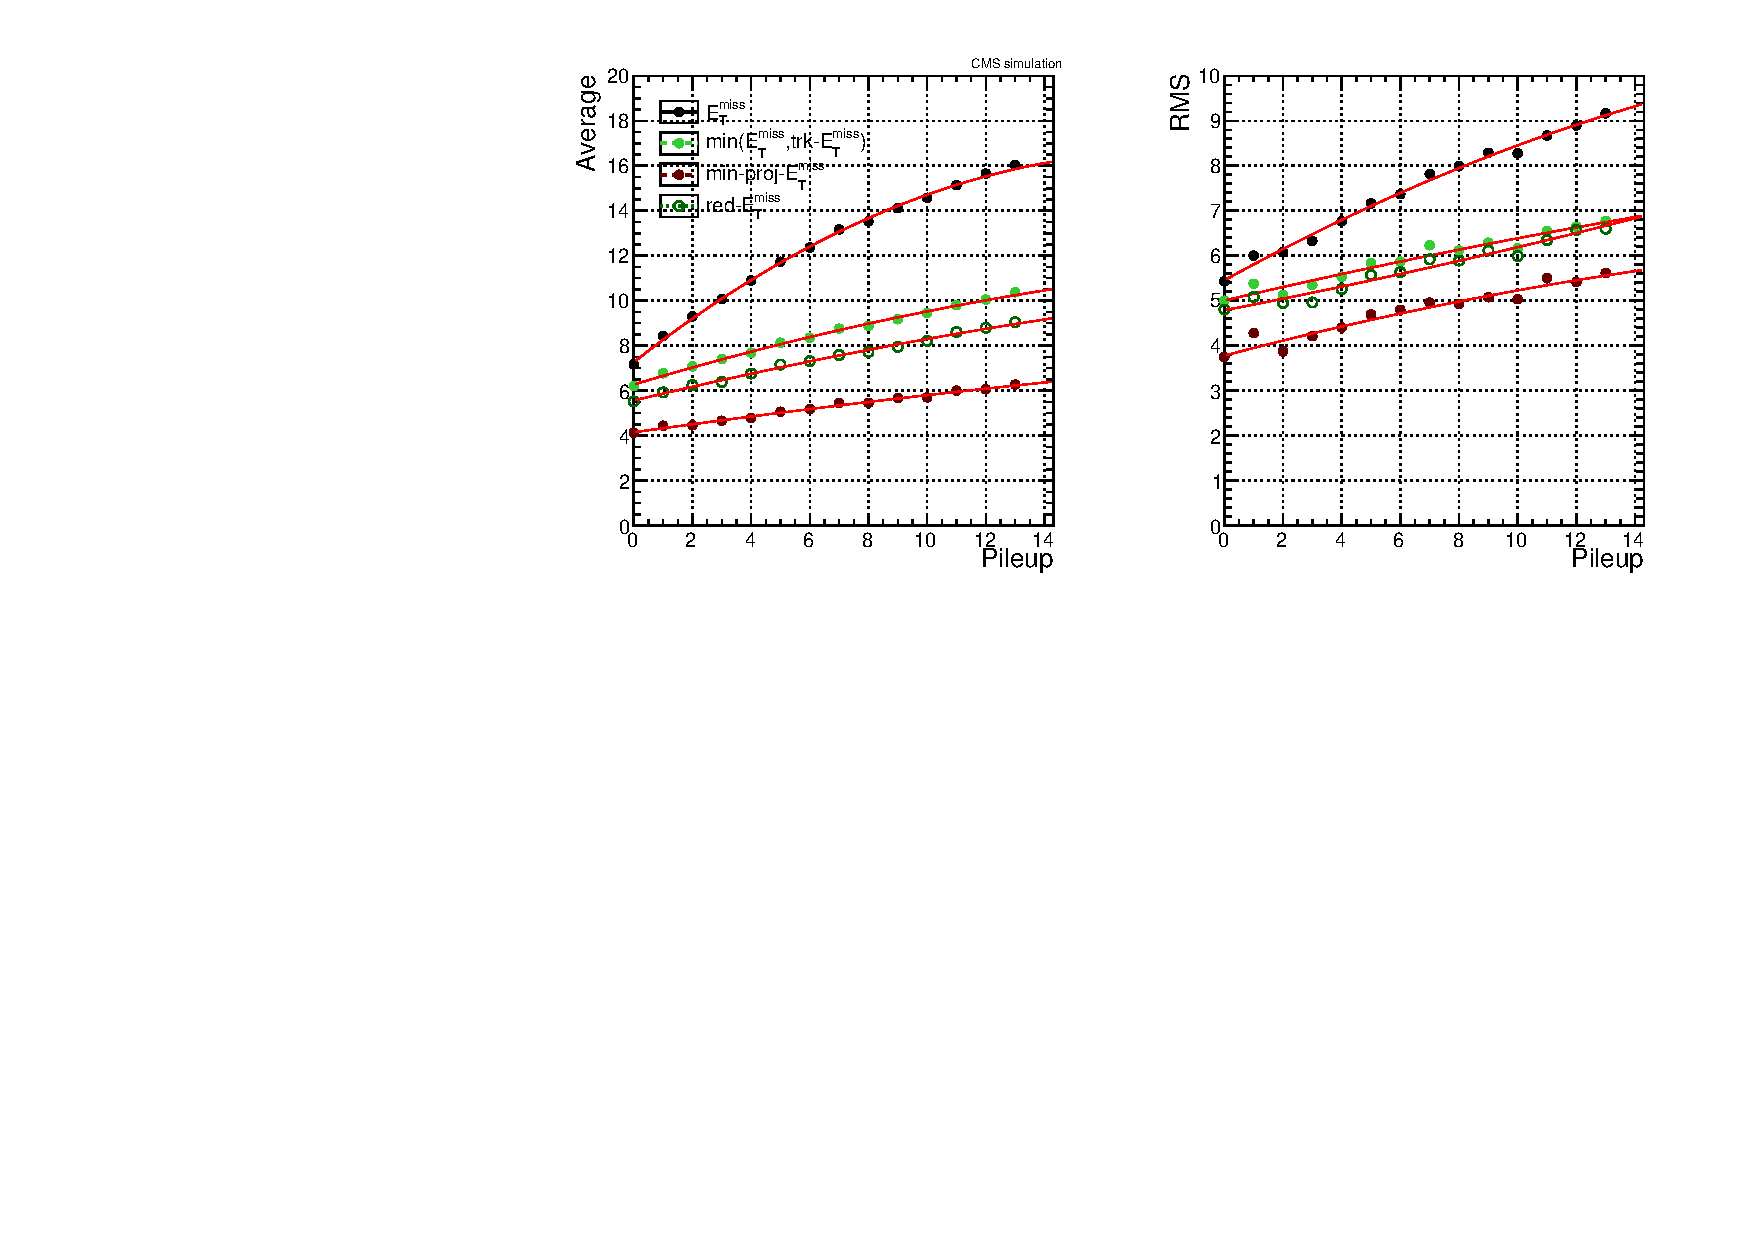
\includegraphics[width=0.9\textwidth]{img/metvariablesVsPileup_zsideband}
\caption{Average ({\em left}) and RMS ({\em right}) of the distribution of different \MET related variables in $Z/#gamma^{*}\rightarrow ll$ events, as function of the pileup.
The {\em top} plots show the results obtained in the Z-boson mass region while the {\em bottom} plots show the results obtained in the side-band region.}
\label{fig:metperformancevspileup}
\end{center}
\end{figure}

In the next sub-section we discuss further strategies which are still subject of on-going studies which attempt 
to minimize further the dependence of these variables against pileup.

%%%
%%% Pileup
%%%
\subsection{Strategies adopted to minimize the effect of pileup}
\label{subsec:pueffects}

In the previous section it was noticed that by taking the minimum for each event of the \MET measurement and the \tkMET measurement
we can obtain an estimate of the \MET which is more robust against the contamination from pileup.
The drawback of this approach is the lost of resolution in the measurement as \tkMET uses only the charged component of the event
which can be measured up to a pseudo-rapidity of $|\eta|<$2.5 due to the limited acceptance of the tracker.
However for the signal we're interested in we expect that the neutrinos are indeed emitted in the central region of the detector
and therefore we expect a correlation between \MET measured using the information from the full detector and \MET measured using the central region.
For instrumental background this is not the case any longer, as depicted in Fig.~\ref{fig:metandtkmet}.
Therefore we explore in this section a strategy to control further the measurement of \MET using the central part of the CMS detector only.

\begin{figure}[htp]
\begin{center}
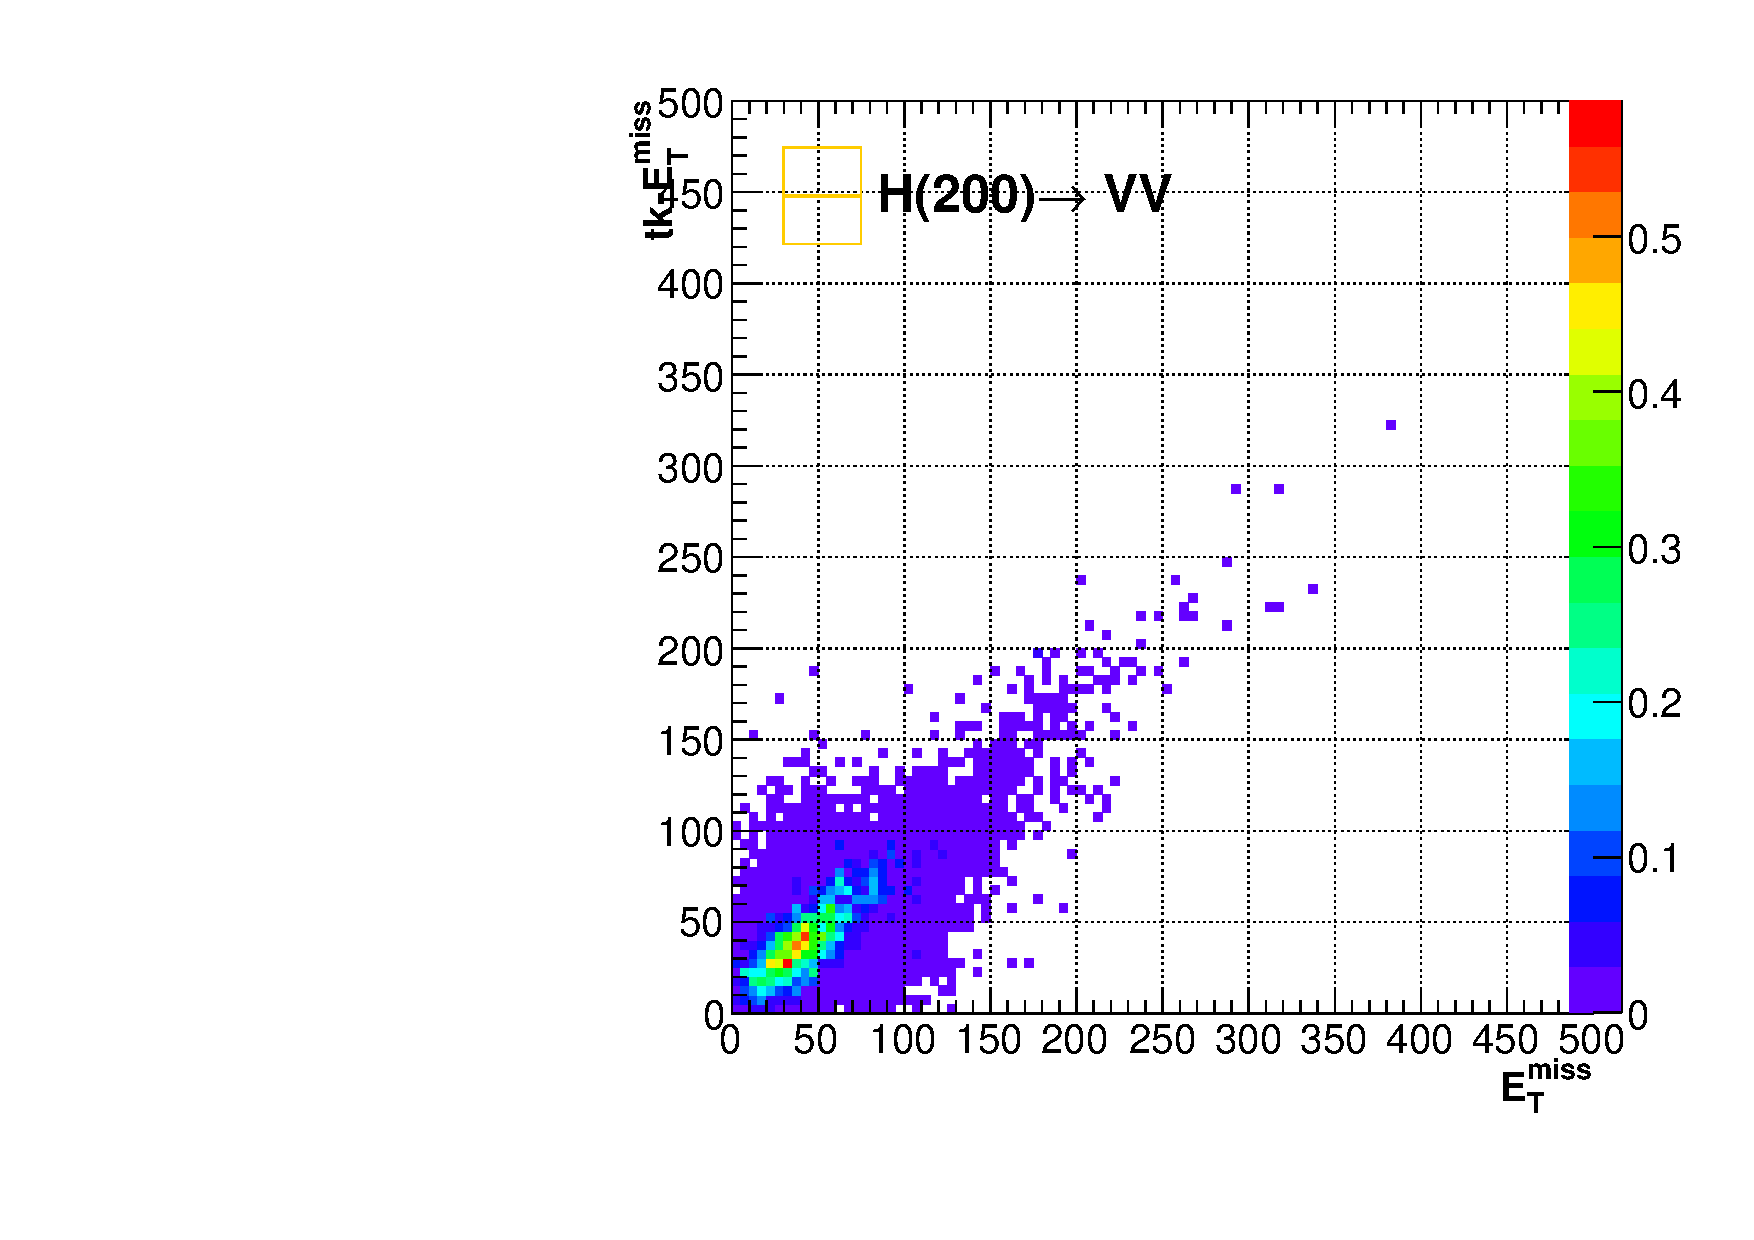
\includegraphics[width=0.45\textwidth]{img/metvstkmet_h200}
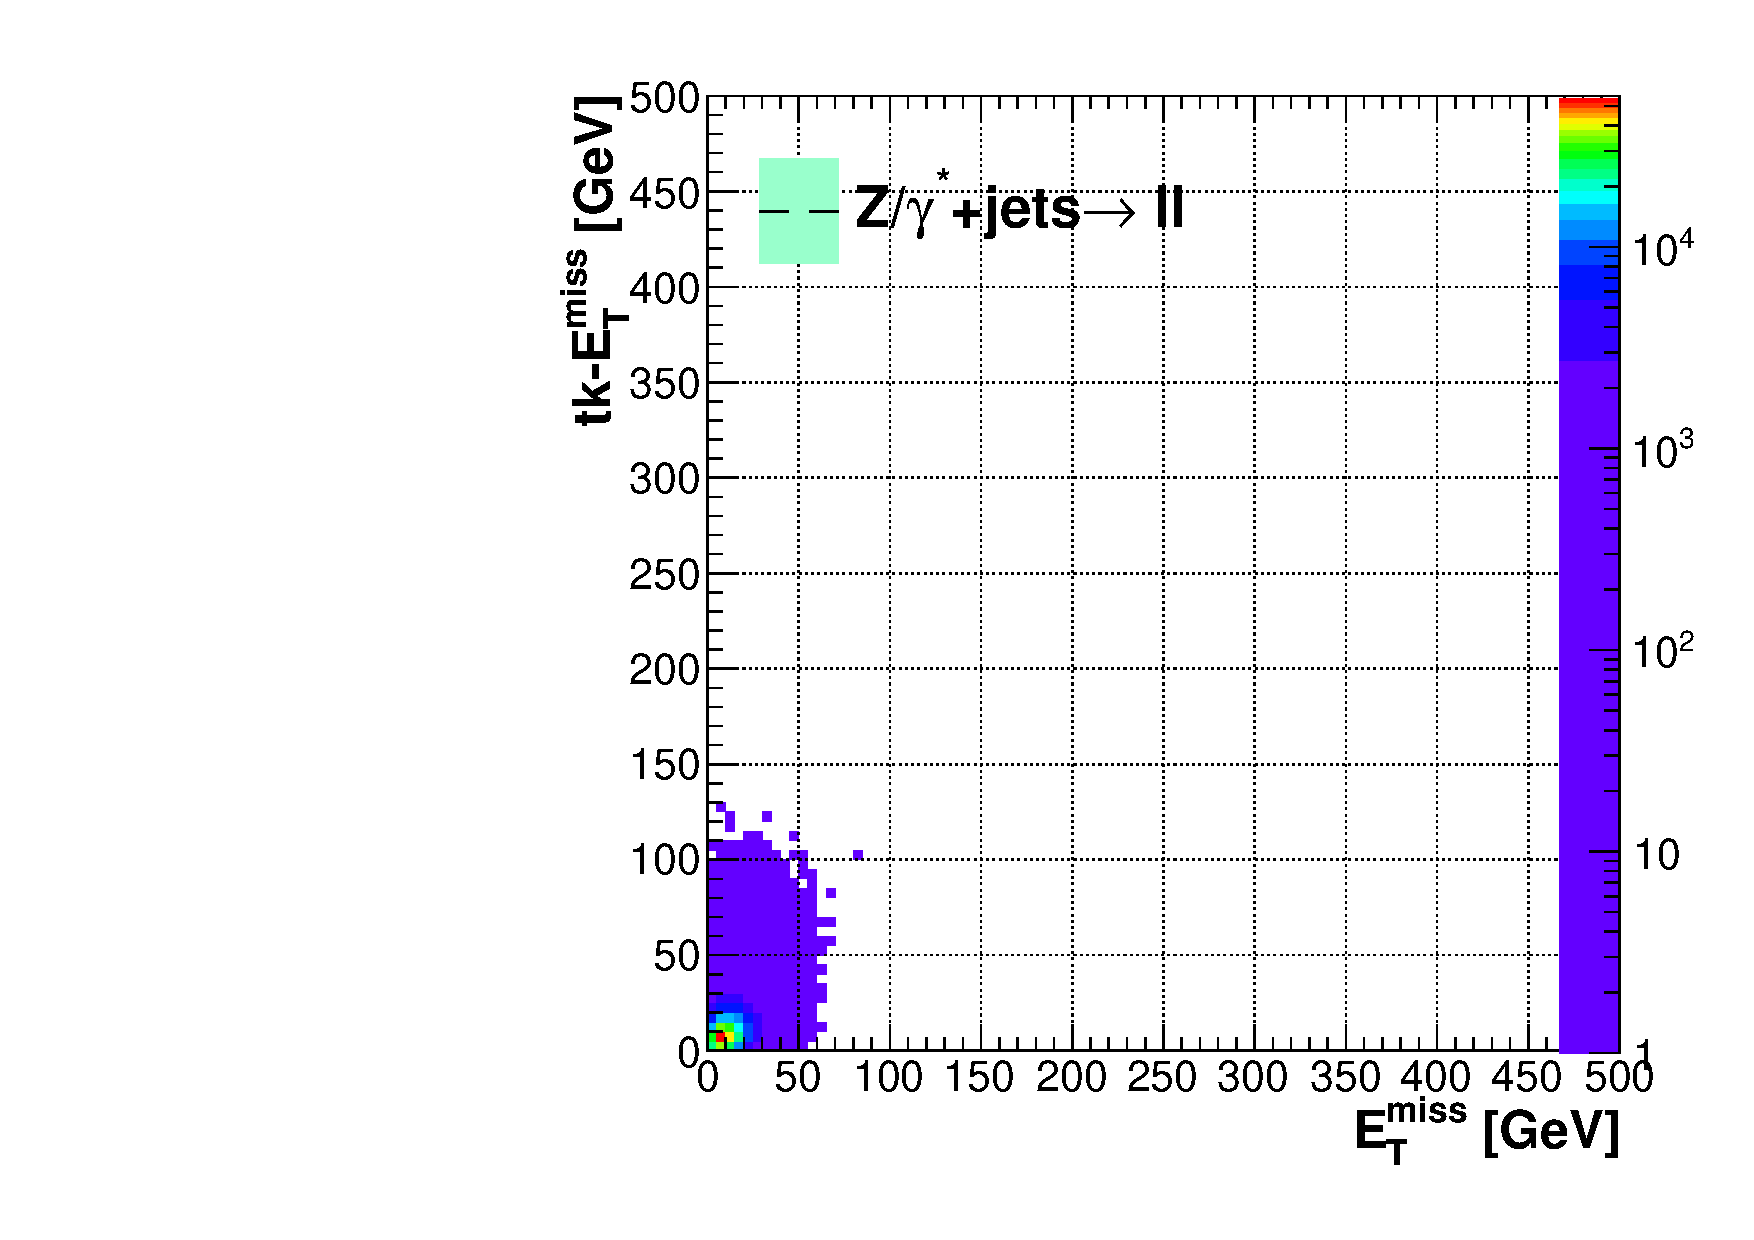
\includegraphics[width=0.45\textwidth]{img/metvstkmet_dy}
\caption{Correlation between \MET and \tkMET for a simulated Higgs (m=200~GeV/c$^2$) sample ({\em left}) and a $Z\rightarrow ll$ sample ({\em right}) in the di-muon sample}.
\label{fig:metandtkmet}
\end{center}
\end{figure}


\begin{table}[htp]
\caption{Definitions used for the different \MET approaches compared in this study.
The particles (not) used in the computation of each \MET type are signaled with ($\Box$) $\blacksquare$.}
\label{tab:pumettypes}
\begin{center}
\begin{tabular}{lllllll} \hline\hline
\multicolumn{2}{c}{\multirow{2}{*}{Particles}}           & \multicolumn{5}{c}{\MET type}                             \\ 
&                                                        & \MET           & \tkMET         & \neutMET       & \clusMET       & \resMET   \\\hline
\multirow{2}{*}{charged}  & all                          & $\blacksquare$ & $\Box$  & $\Box$  & $\Box$  & $\Box$          \\
                          & assoc. vertex                & $\Box$  & $\blacksquare$ & $\Box$  & $\blacksquare$ & $\blacksquare$       \\\hline
\multirow{2}{*}{neutrals} & all                          & $\blacksquare$ & $\Box$  & $\blacksquare$ & $\Box$  & $\Box$          \\
                          & assoc. to vertex-seeded jets & $\Box$  & $\Box$  & $\Box$  & $\blacksquare$ & $\blacksquare$       \\
                          & assoc. to other jets         & $\Box$  & $\Box$  & $\Box$  & $\Box$  & $\Box$        \\\hline\hline
\end{tabular}
\end{center}
\end{table}

%
%
%
\section{Search for the standard model Higgs in the 2l2$\nu$ final state}
\label{sec:higgssearch}

The next Sections describe three complementary approaches to search for the standard model Higgs in the 2l2$\nu$ final state.
The analysis rely on the expected behavior for Higgs events as described in the simulation. 
Two of the analysis are cut-based and a third one is a discriminator based analysis implemented using the TMVA package~\cite{Hocker:2007ht}.
For each analysis the events are categorized according to the jet multiplicity observed.
Events with $\geq$2~jets are furthermore analyzed to search for the vector-boson-fusion (VBF) specific signature.
This is will be described in more detail in the next sub-section. If the event does not meet the VBF specific selection
it is accounted for in the $\geq$2~jets bin.

%%
%% VBF selection
%%
\subsection{Vector Boson Fusion search}
\label{subsec:vbfsearch}



%%
%% Higgs event selection
%%
\subsection{Higgs event selection using a cut-based analysis approach}
\label{subsec:higgsselection}

The selection variables chosen for the search of the Higgs boson production in the gg$\rightarrow$H mode are summarized in Tab.~\ref{tab:gluglucuts}.
The cuts were chosen my maximing a simple figure of merit $f=S/\sqrt(S+B)$ after requiring that the instrumental $Z$ background
is reduced by a 10$^{-3}$ (medium \RMET working point).
The details on the $f$ variable can be found in Sec.~\ref{sec:app:cutbasedoptimization}.

\begin{table}[htp]
\caption{Selection variables for the search for the Higgs boson in the gg$\rightarrow$H mode.}
\label{tab:gluglucuts}
\begin{center}
\begin{tabular}{cccc} \hline\hline
\multirow{2}{*}{Higgs mass (GeV/c$^2$)} & \multicolumn{3}{c}{Variable} \\
                            & $\delta\phi^{ll}$ & \RMET (longitudinal) & $\sum M_T$ \\ \hline
200                         & 1.0$<|x|<$2.75  & $|x|>$50             & $>$150 \\
300                         & $|x|<$2.5         & x$>$75               & $>$200 \\
400                         & $|x|<$2.0         & x$>$75               & $>$300 \\
500                         & $|x|<$2.0         & x$>$100              & $>$400 \\
600                         & $|x|<$1.5         & x$>$150              & $>$400 \\\hline\hline
\end{tabular}
\end{center}
\end{table}


%%
%% Discriminator analysis
%%
\subsection{Discriminator based analysis of the selected events}
\label{subsec:discanalysis}

%%
%%
%%
\subsection{Efficiency of the selection}
\label{subsec:selefficiency}


%%
%% Background determination
%%
\subsection{Background determination}
\label{subsec:backgrounddet}


%%%
%%% Instrumental background
%%%
\subsubsection{Data-driven estimation of the instrumental background}
\label{subsubsec:instrumentalbackground}

Photon candidates are selected from dedicated photon triggered samples.
The samples are summarized in Table~\ref{tab:instrbckgdatasamples}.

\begin{table}[htp]
\begin{center}
\caption{\MC and data samples analyzed for the estimation of the instrumental background.
For data the total integrated luminosity and the run range analyzed are shown.
For \MC the the cross section and the corresponding integrated luminosity of the analyzed sample are shown.
Z2 is used as a shortname for TuneZ2\_7TeV\_pythia6 and S* for Summer11-PU\_S*\_START42\_V11.
}          
\label{tab:instrbckgdatasamples}
\begin{tabular}{lcl} \hline\hline
\multicolumn{3}{c}{\bf Data} \\
Dataset                               & $L$~(pb$^{-1}$)               & Run range                          \\\hline
/Photon/Run2011A-May10ReReco-v1/AOD   &                               & {\small 160404-163869}             \\
/Photon/Run2011A-PromptReco-v4/AOD    &                               & {\small $>$163869}                 \\
{\bf Total}                           & {\bf }                        &                                    \\\hline
                                      &                               &                                    \\\hline
\multicolumn{3}{c}{\bf \MC} \\
Dataset                               & $\sigma$~(pb)                 & $L$~(pb$^{-1}$)                   \\\hline
/G\_Pt-15to30\_Z2/S3-v2/AODSIM        & 1.72$\times$10$^5$            &                                   \\
/G\_Pt-30to50\_Z2/S3-v2/AODSIM        & 1.67$\times$10$^4$            &                                   \\
/G\_Pt-50to80\_Z2/S3-v2/AODSIM        & 2.72$\times$10$^3$            &                                   \\
/G\_Pt-80to120\_Z2/S4-v2/AODSIM       & 4.47$\times$10$^2$            &                                   \\
/G\_Pt-120to170\_Z2/S3-v2/AODSIM      & 84.2                          &                                   \\
/G\_Pt-170to300\_Z2/S4-v2/AODSIM      & 22.6                          &                                   \\
/G\_Pt-300to470\_Z2/S3-v2/AODSIM      & 1.49                          &                                   \\
/G\_Pt-470to800\_Z2/S3-v2/AODSIM      & 0.132                         &                                   \\
/G\_Pt-800to1400\_Z2/S3-v2/AODSIM     & 3.48$\times$10$^{-3}$         &                                   \\
/G\_Pt-1400to1800\_Z2/S3-v2/AODSIM    & 1.26$\times$10$^{-5}$         &                                   \\\hline\hline
\end{tabular}
\end{center}
\end{table}

For each triggered event the highest $p_T$ photon trigger candidate is chosen.
The offline reconstructed photon is required to have a $E_T$ 
greater than that of the trigger threshold it fired.
Further identification and isolation requirements are made as summarized in Table~\ref{tab:photonsel}
and are based on~\cite{Khachatryan:2010fm}.

\begin{table}[htp]
\begin{center}
\caption{Photon selection requirements according to the region of reconstruction in the electromagnetic calorimeter.}
\label{tab:photonsel}
\begin{tabular}{lcc} \hline\hline
Variable                              & ECAL barrel                        & ECAL endcap                   \\\hline
$E_T$                                 & \multicolumn{2}{c}{trigger dependent}                              \\
$|\eta|$                              & $<$1.4442                          & 1.566$<|\eta|<$2.5            \\ 
$\sigma_{i\eta i\eta}$                & 0$<\sigma<$0.013                   & 0$<\sigma<$0.03               \\ 
$\sigma_{i\phi i\phi}$                & $>$0                               & -                             \\ 
seed rec. hit flag                    & $\neq$ kOutOfTime                  & -                             \\ 
$h/e$                                 & $<$0.05                            & $<$0.5                        \\ 
Tracker isolation                     & \multicolumn{2}{c}{$<$2.0 + 0.001$E_T$}                            \\ 
ECAL isolation                        & \multicolumn{2}{c}{$<$4.2 + 0.003$E_T$}                            \\ 
HCAL isolation                        & \multicolumn{2}{c}{$<$2.2 + 0.001$E_T$}                            \\\hline 
\end{tabular}
\end{center}
\end{table}

%%%
%%% Top 
%%%
\subsubsection{Data-driven estimation of residual top background}
\label{subsubsec:topbackground}

%%
%%
%%
\subsection{Systematic uncertainties}
\label{subsec:systunc}


%
%
%
\section{Exclusion limits}
\label{sec:excllimits}


%
% CONCLUSIONS
%
\section{Conclusions}
\label{sec:conclusions}

%% **DO NOT REMOVE BIBLIOGRAPHY**
\bibliography{auto_generated}   % will be created by the tdr script.

\clearpage
%
% APPENDIX
%
\appendix
\section{Appendix: Lepton isolation}
\label{sec:app:leptonisolation}

In this section we focus on two specific aspects affecting the determination of lepton isolation efficiency:
the contamination from pileup and the differences between leptons in the $Z\rightarrow ll$ sample and in the Higgs sample.

The presence of pileup is expected to contribute to the degradation of the isolation, especially 
through the neutral particles which cannot be associated to the vertex.
The deviation introduced in the isolation by the average energy density deposition in the detector from pileup
can be estimated using the $\rho$-parameter computed using the fast jet algorithm~\cite{Cacciari:2007fd}.
As the average values for $\rho$, $I_{photons}$ and $I_{neutral~hadrons}$ are expected to increase differently as a function of the number of pileup events
a linear parameterization can be derived for each case and used to correct the isolation in average.
The results of these parameterizations are shown for in Fig~\ref{fig:isolprofile} for a simulated sample of $Z\rightarrow \mu\mu$.
The width of the distributions of the previous variables is also affected by the pileup and in the case of the $\rho$ a non-linear behavior is observed.
In this study we choose therefore not to perform any correction for the isolation based on the pileup contamination as estimated from 
the $\rho$ parameter due to the fact that events with large fluctuations of $\rho$ can lead to overcorrections of the lepton isolation leading to an increase
of the contamination from non-isolated lepton candidates.
The slope of the isolation profile is used to assign a systematic uncertainty on the isolation efficiency of 0.8\%
for both electrons and muons.

\begin{figure}[htp]
\begin{center}
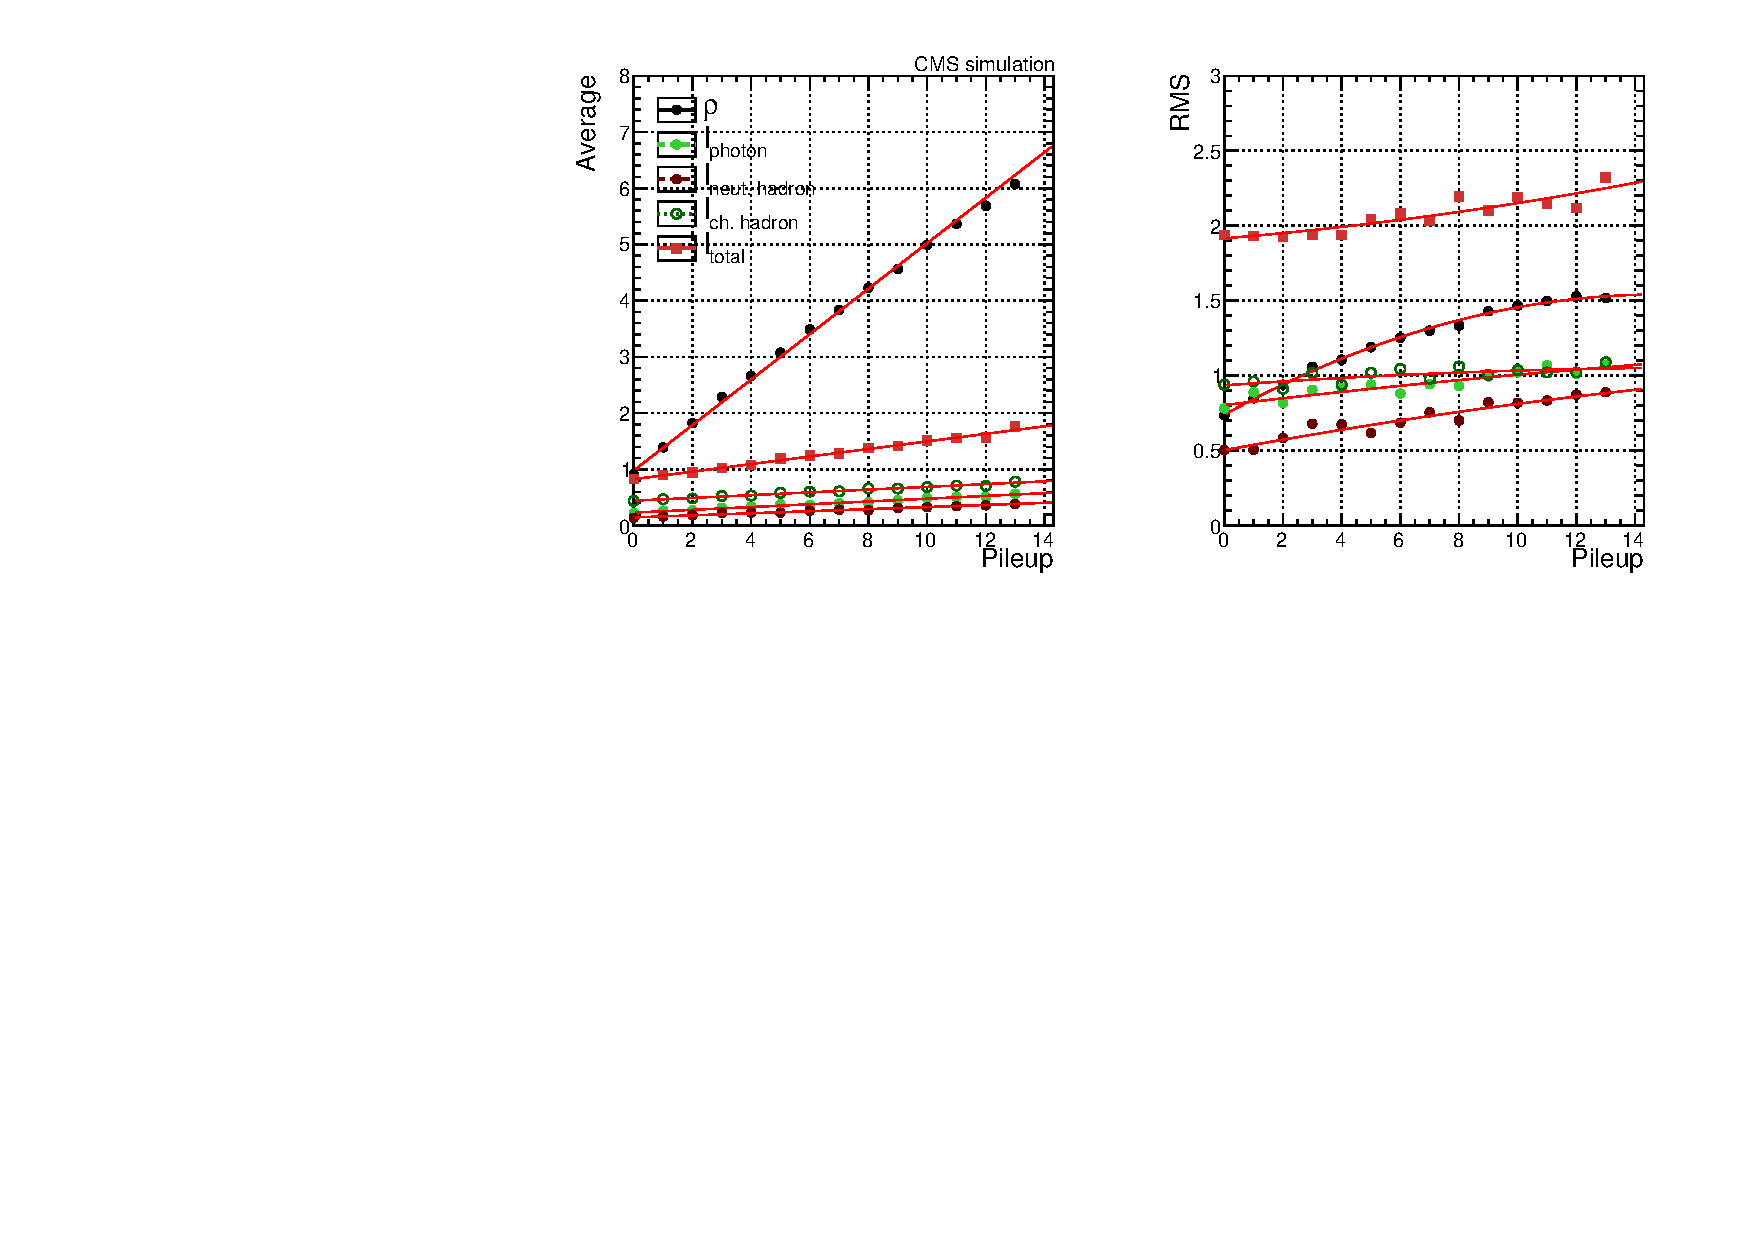
\includegraphics[width=0.9\textwidth]{img/muonIsolationProfile}
\caption{
Isolation and $\rho$ profiles in simulated $H\rightarrow VV\rightarrow 2\mu 2\nu_{\mu}$ events.
The average (RMS) of the distributions is shown as function of the number of generated pileup events on the {\em left} ({\em right}).}
\label{fig:isolprofile}
\end{center}
\end{figure}

The efficiency of the isolation requirement is determined from data using the tag-and-probe method.
This method relies on the kinematics of $Z\rightarrow ll$ events which may differ slightly from the kinematics
of the signal, i.e. $H\rightarrow VV\rightarrow 2l2\nu$. The difference is not expected to be observed in the absolute isolation of the leptons
as the jet activity is not substantially different and as the pileup conditions are similar.
However, as the $p_T$ distribution of the leptons is different, being the leptons from $Z$ events usually softer, 
a difference arises in the relative isolation, as the ratio of the absolute isolation to the $p_T$ of each lepton is considered.
This effect is illustrated in Fig.~\ref{fig:zvshlepkinematics} where the $p_T$, absolute isolation and relative isolation
of the leptons matched to the decays of the Z bosons are compared. 
From this study we conclude that the efficiency of the relative isolation in $\mu\mu$ ($ee$) events is 0.8\% (0.5\%) smaller in Higgs events with respect to $Z$ events. 
Therefore we assign this number as a systematic uncertainty on the efficiency computed from data using the tag-and-probe method. 

\begin{figure}[htp]
\begin{center}
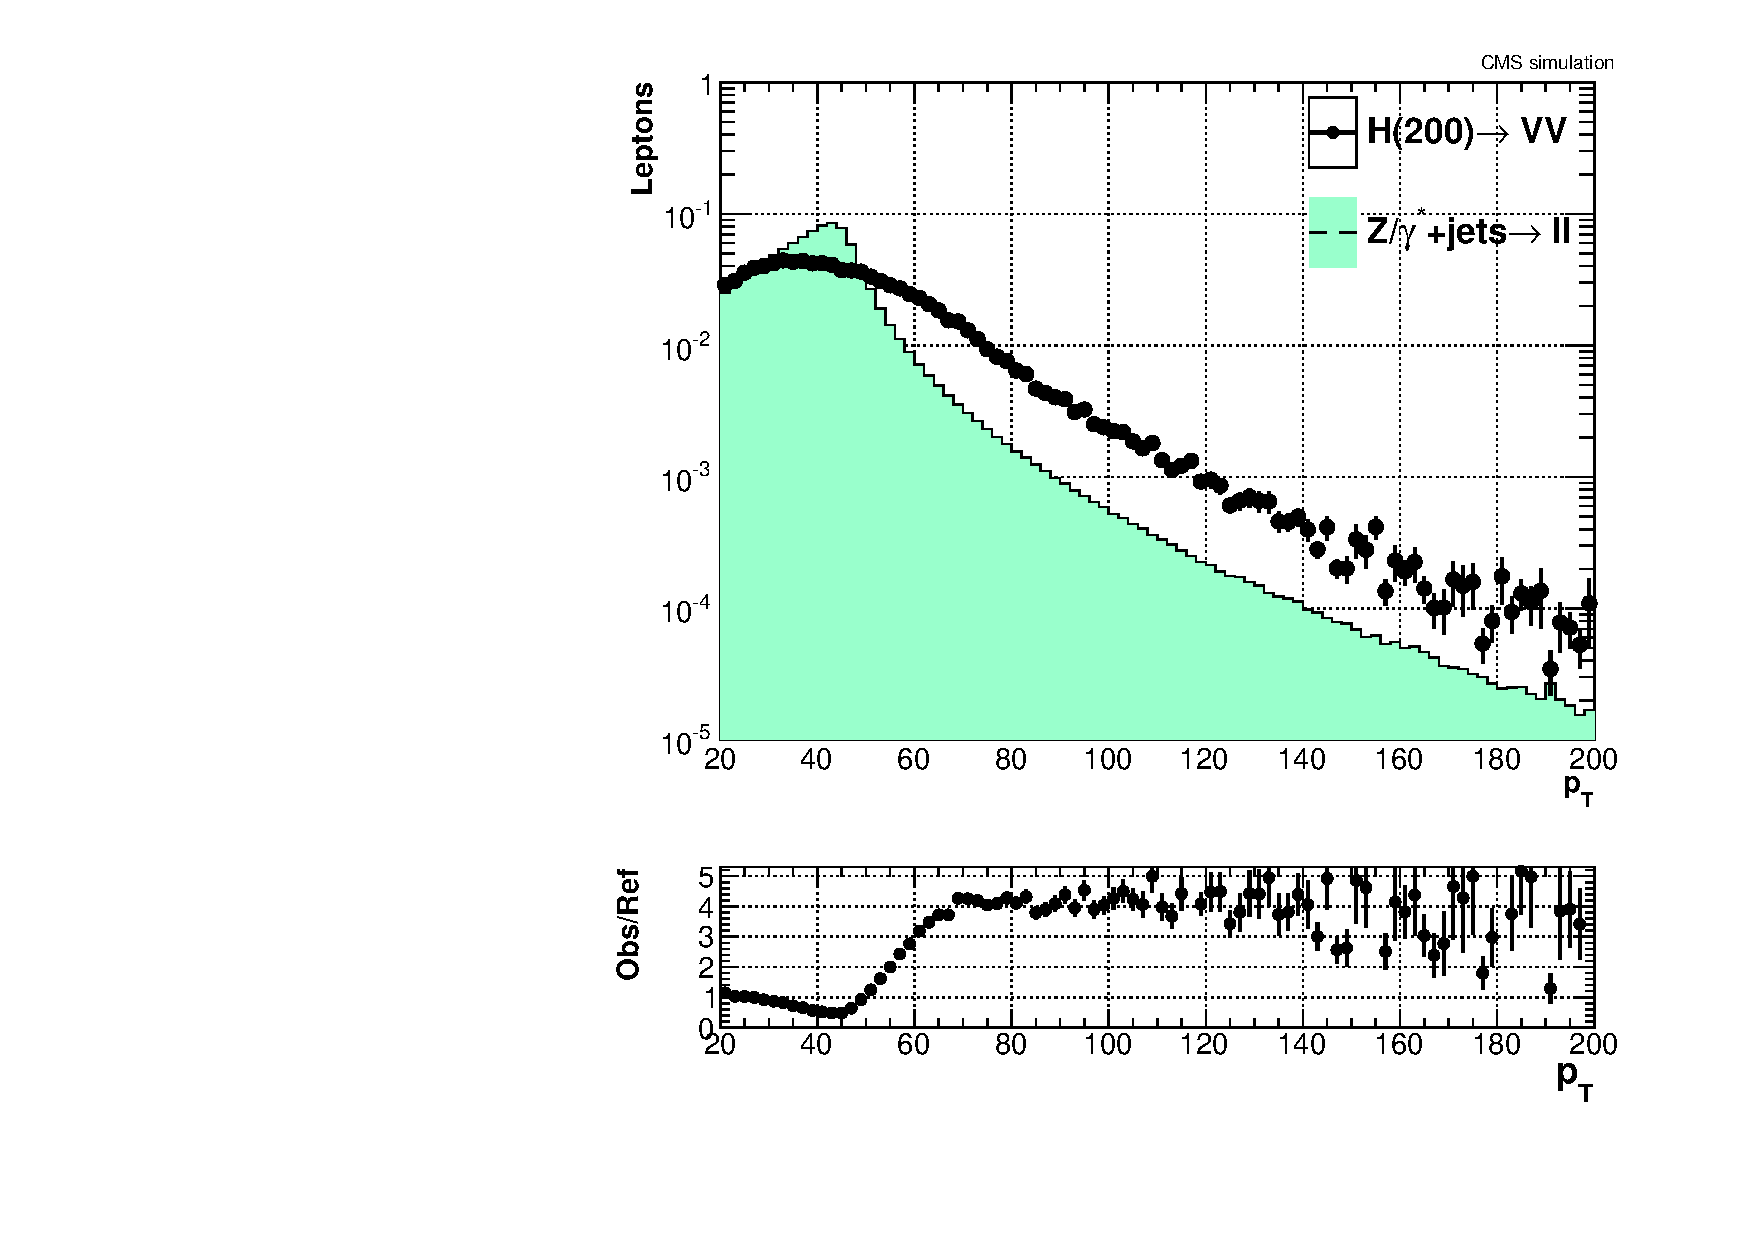
\includegraphics[width=0.3\textwidth]{img/matchedmuon_pt}
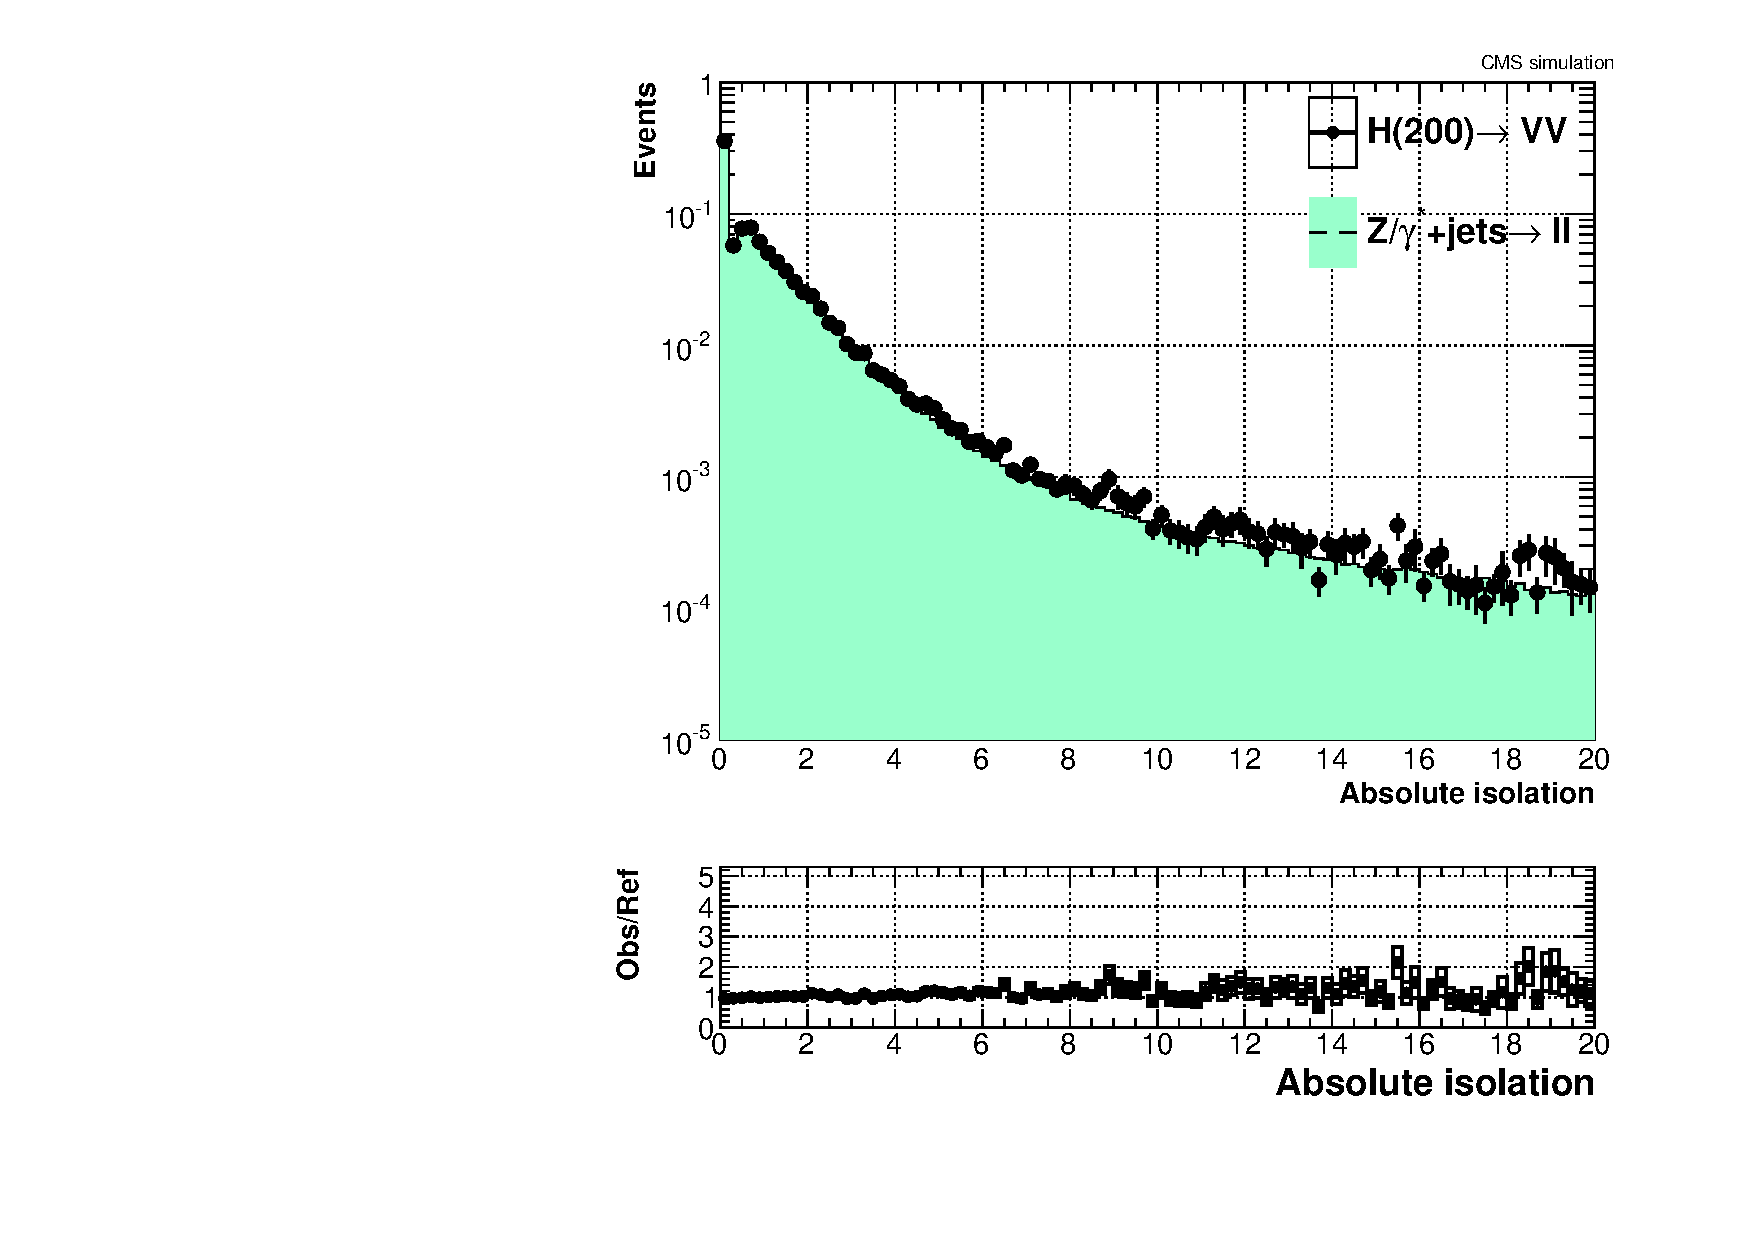
\includegraphics[width=0.3\textwidth]{img/matchedmuon_absiso}
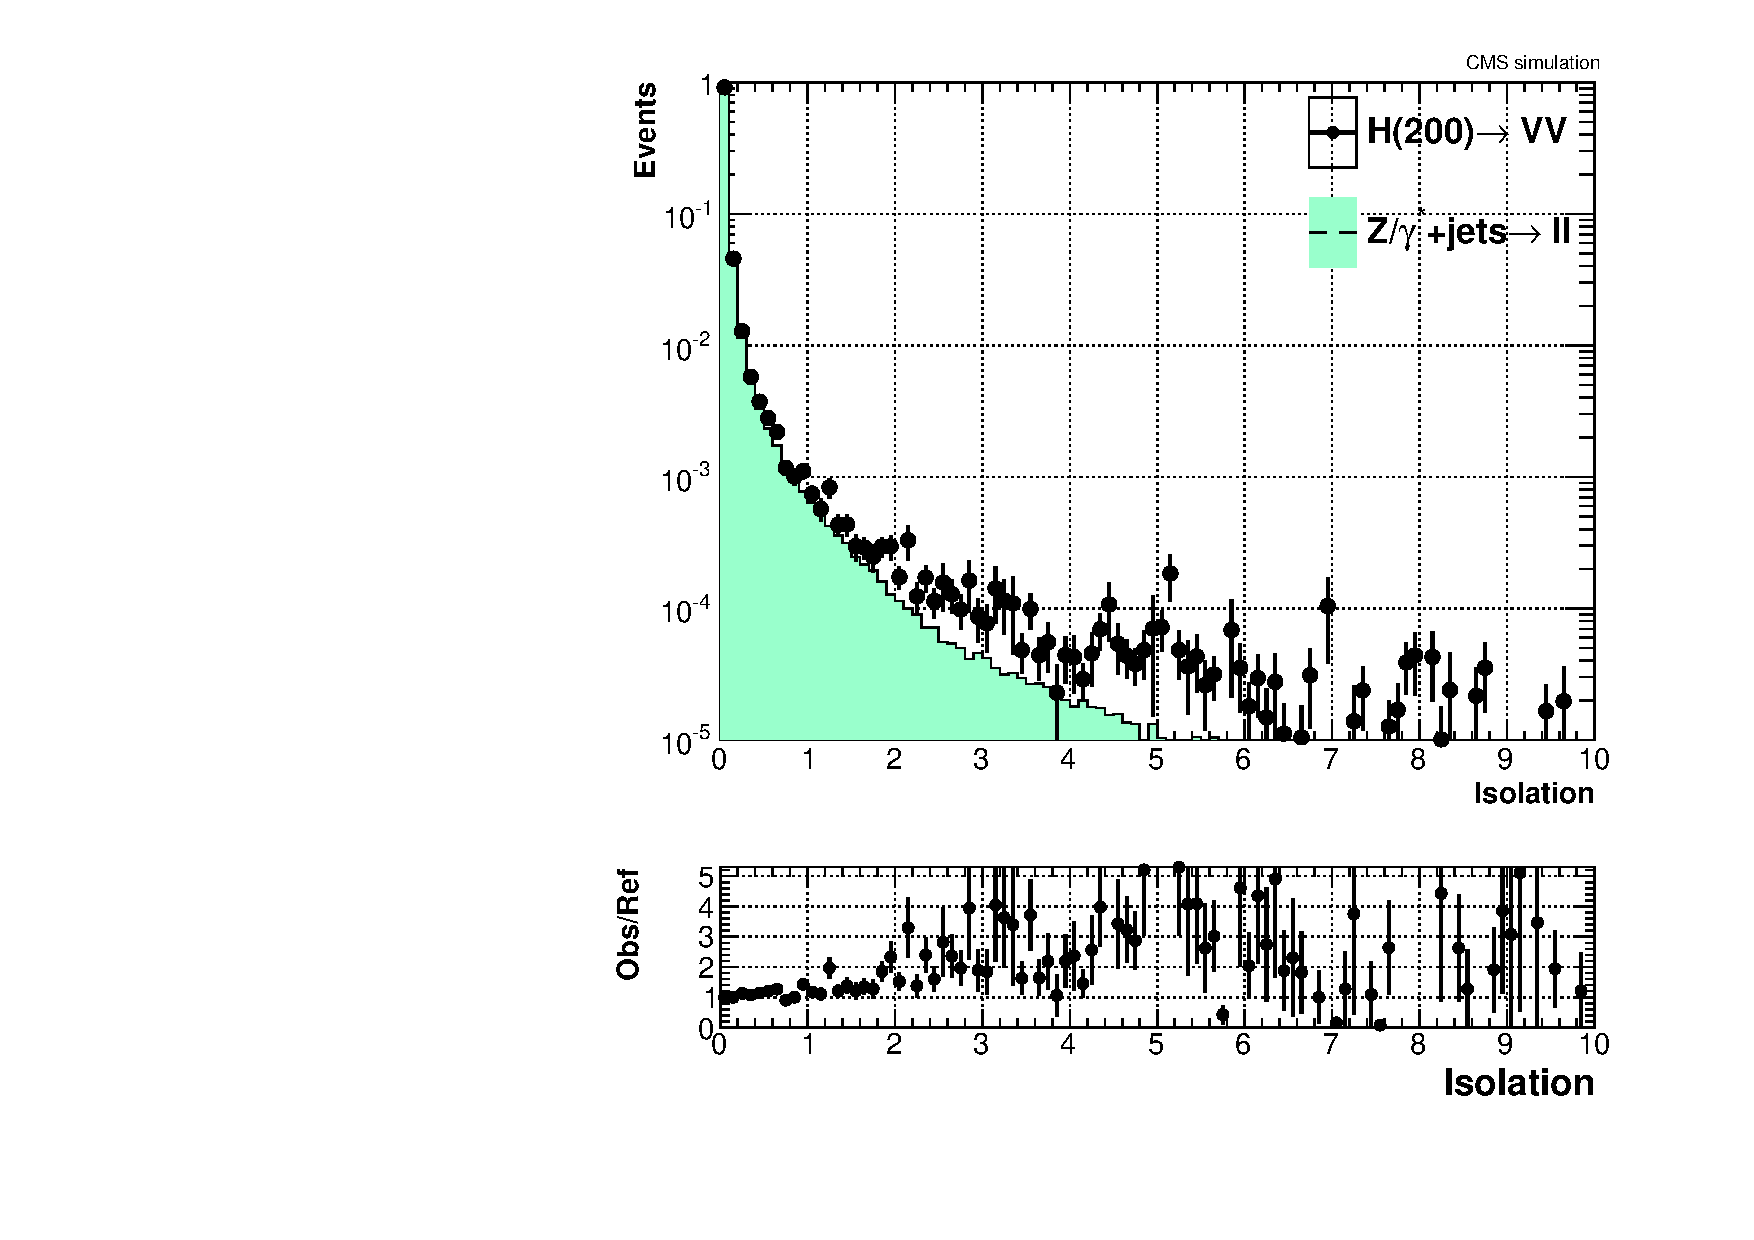
\includegraphics[width=0.3\textwidth]{img/matchedmuon_reliso}\\
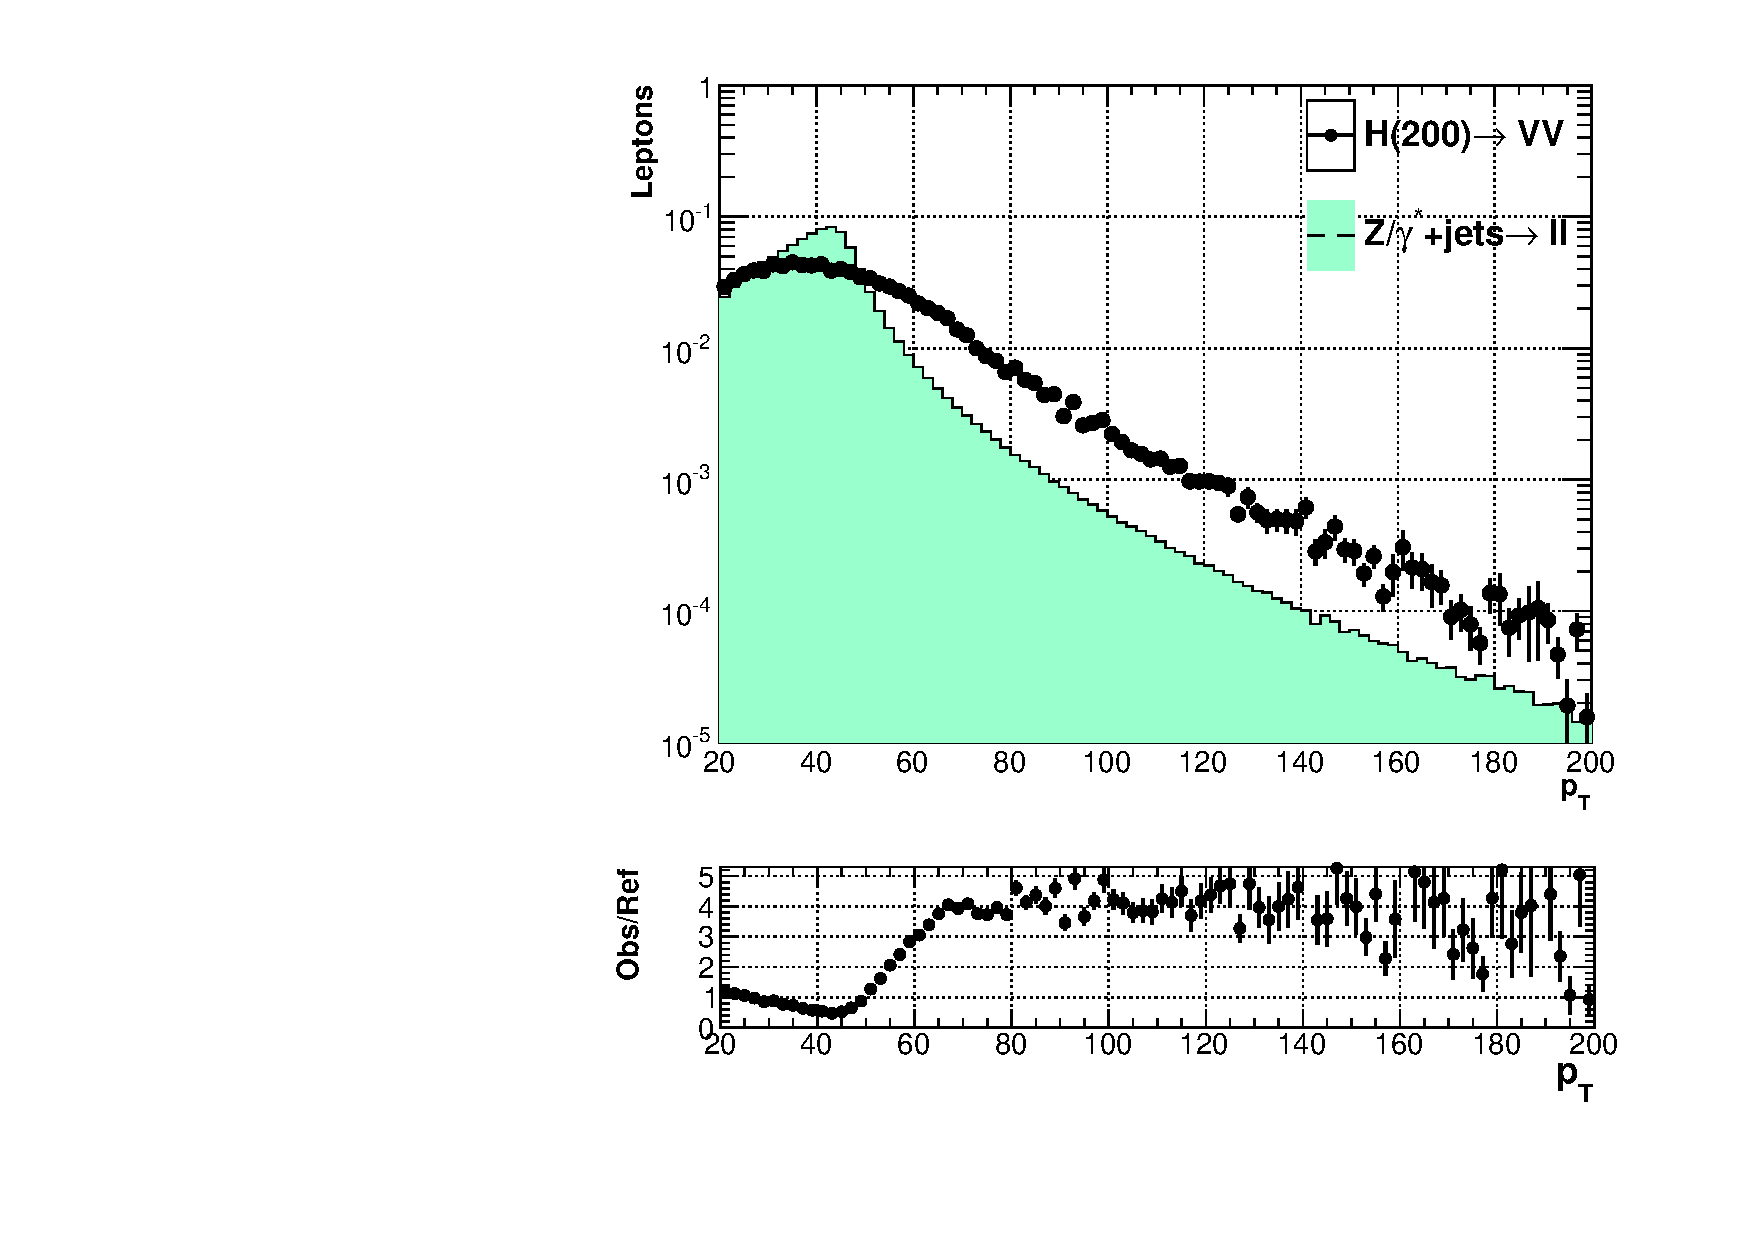
\includegraphics[width=0.3\textwidth]{img/matchedelectron_pt}
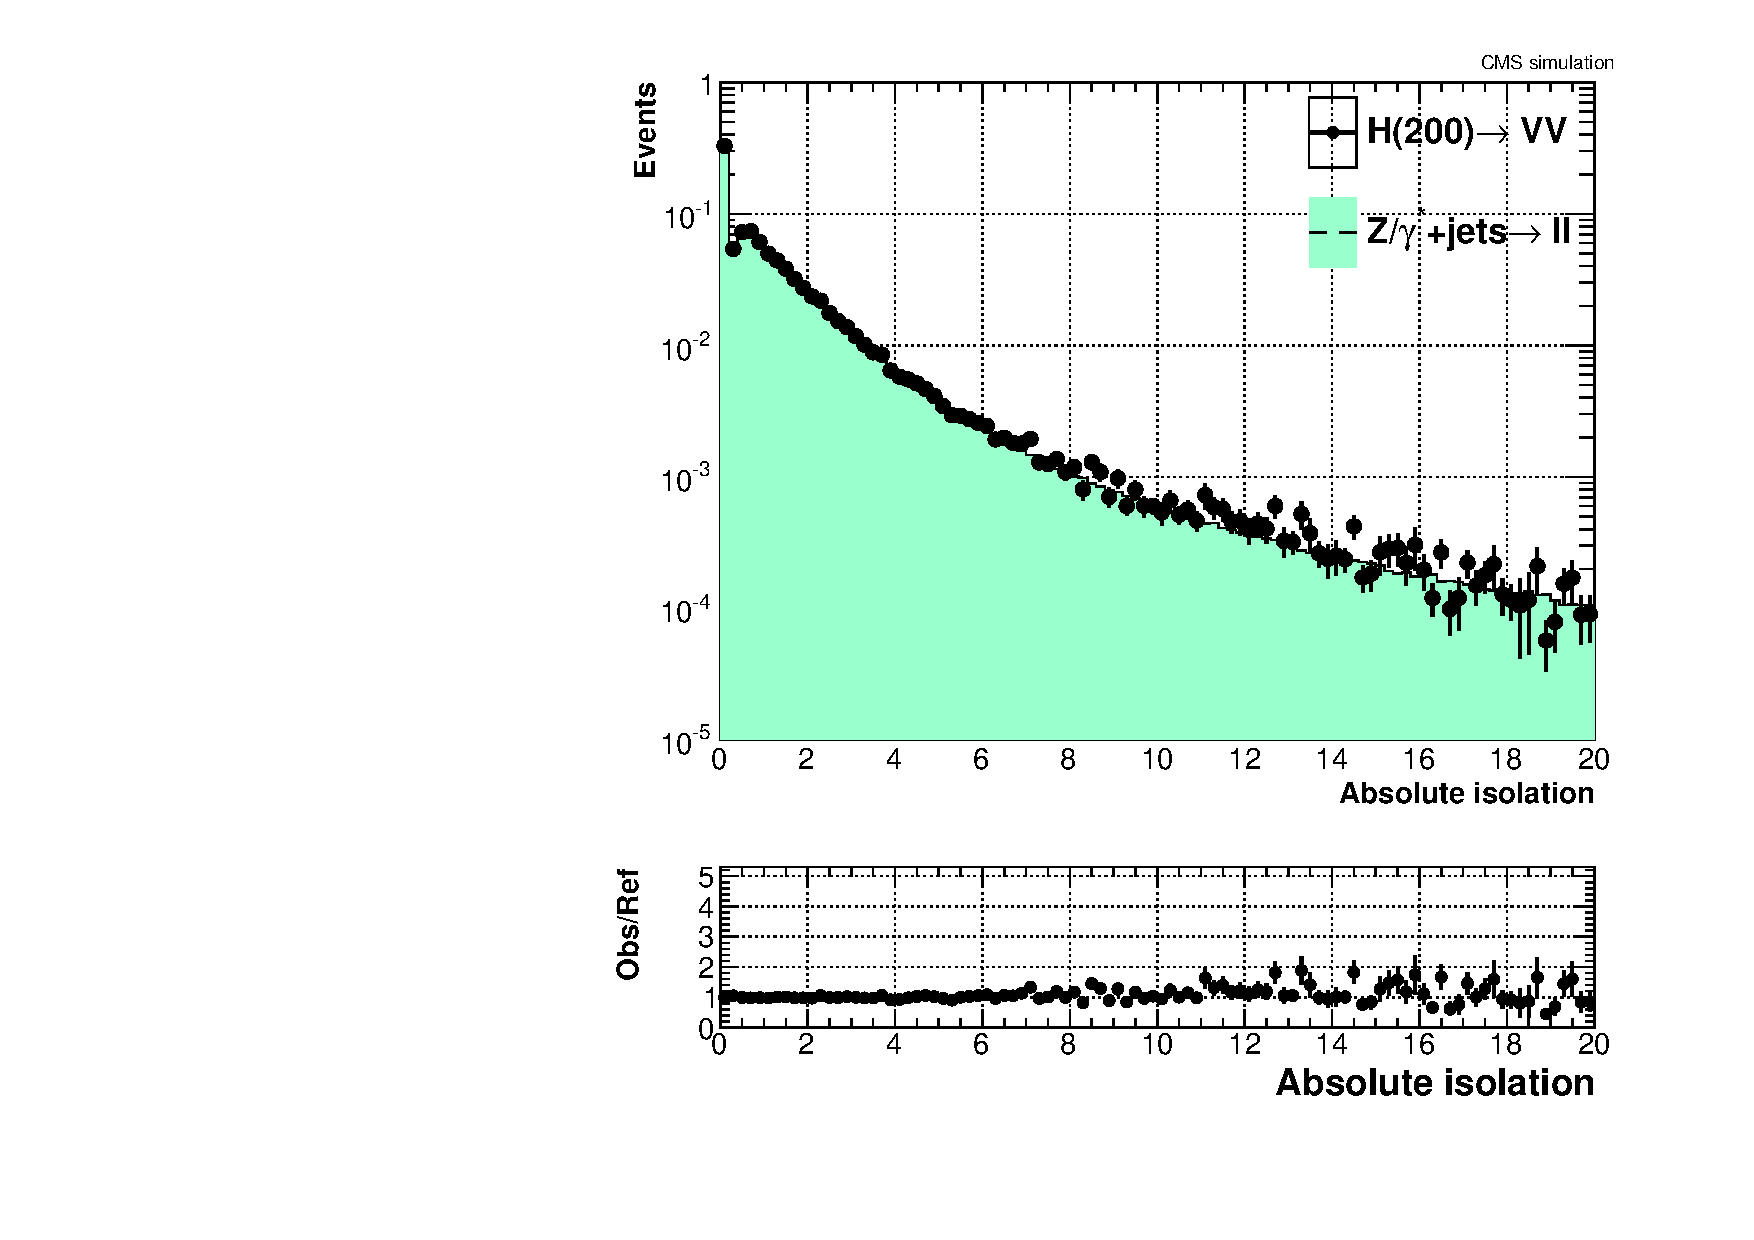
\includegraphics[width=0.3\textwidth]{img/matchedelectron_absiso}
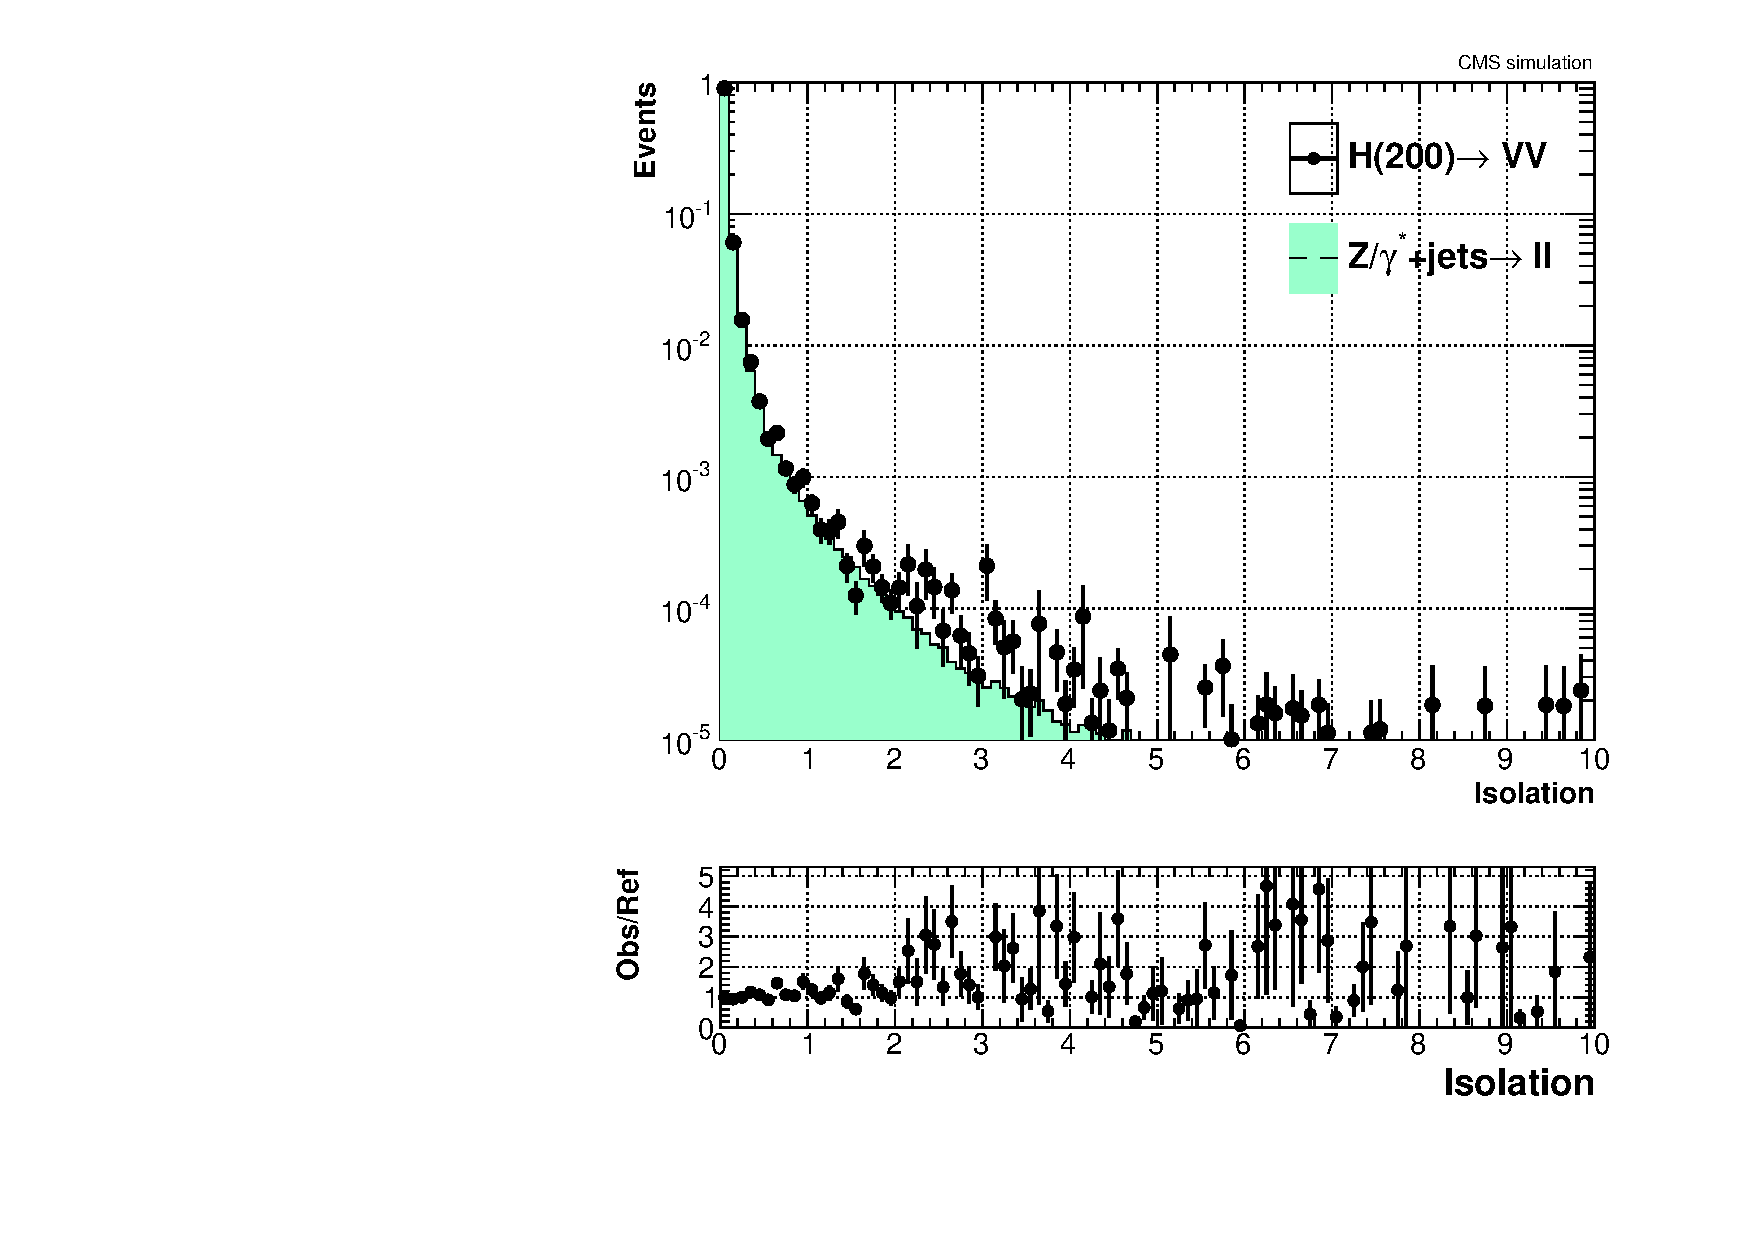
\includegraphics[width=0.3\textwidth]{img/matchedelectron_reliso}
\caption{Transverse momentum ({\em left}), absolute isolation ({\em center}) and relative isolation ({\em right}) of the
reconstructed muons ({\em top}) and electrons ({\em bottom}) matched to the generator level
leptons fro the $Z$ boson decay in simulation.
The standard $Z$ production is compared to the production in the Higgs decay chain considering an hypothetical mass of 200~GeV/c$^2$.}
\label{fig:zvshlepkinematics}
\end{center}
\end{figure}



\section{Appendix: Cut based optimization}
\label{sec:app:cutbasedoptimization}

In this section we summarize the procedure adopted to optimized the selection of the cut based analysis for the search for Higgs boson.
A simple approach has been taken by considering three variables which show discriminating power for the Higgs signal.
These variables are:

\begin{description}
\item[$\delta\phi^{ll}$] - the azimuthal angle between the two leptons that constitute the dilepton candidate. The angle is expected to be significantly smaller for final state leptons from Higgs with large mass;
\item[\RMET (longitudinal)] - the longitudinal component of \RMET. This specific projection is expected to show the sensitivity to events in which the two Z bosons from the Higgs decay are recoiling against each other.
For low mass Higgs, the production of extra jets, might however lead to a boost of the overall system in which both Z's can be produced along the same hemisphere. 
In these boosted topologies the longitudinal component of \RMET is expected to point along the dilepton direction;
\item[$\sum M_{T}(l^i,E_{T}^{miss})$] - the sum of the transverse mass of each lepton with the \MET vector. This variable is chosen as no full mass reconstruction is possible in the final state under study.
The full transverse mass of the system could be used but by requiring both the dilepton and the \MET source to be the same, i.e., a $Z$ boson, introduces an artificial kinematic limit on all backgrounds.;
\end{description}

The  variables used to define a loose selection region where the presence of signal is more significative, i.e. where $f=S/\sqrt{S+B}$ is maximized.
As tighter selections also lead to a depletion of signal, the cuts are selected in the rising edge of the $f$ variable.
Fig.~\ref{fig:varcutopt} summarizes the distributions obtained for the $f$ variable after requiring that the instrumental
background is reduced by 10$^{-3}$ (medium working point for \RMET selection, as defined in Sec.~\ref{subsec:redmet}.
Although differences are found between different jet multiplicity bins, they are not considered to tune further the cuts,
as the $f$-curves show similar rising edges. Therefore, inclusive selection cuts are chosen.

\begin{figure}[htp]
\begin{center}
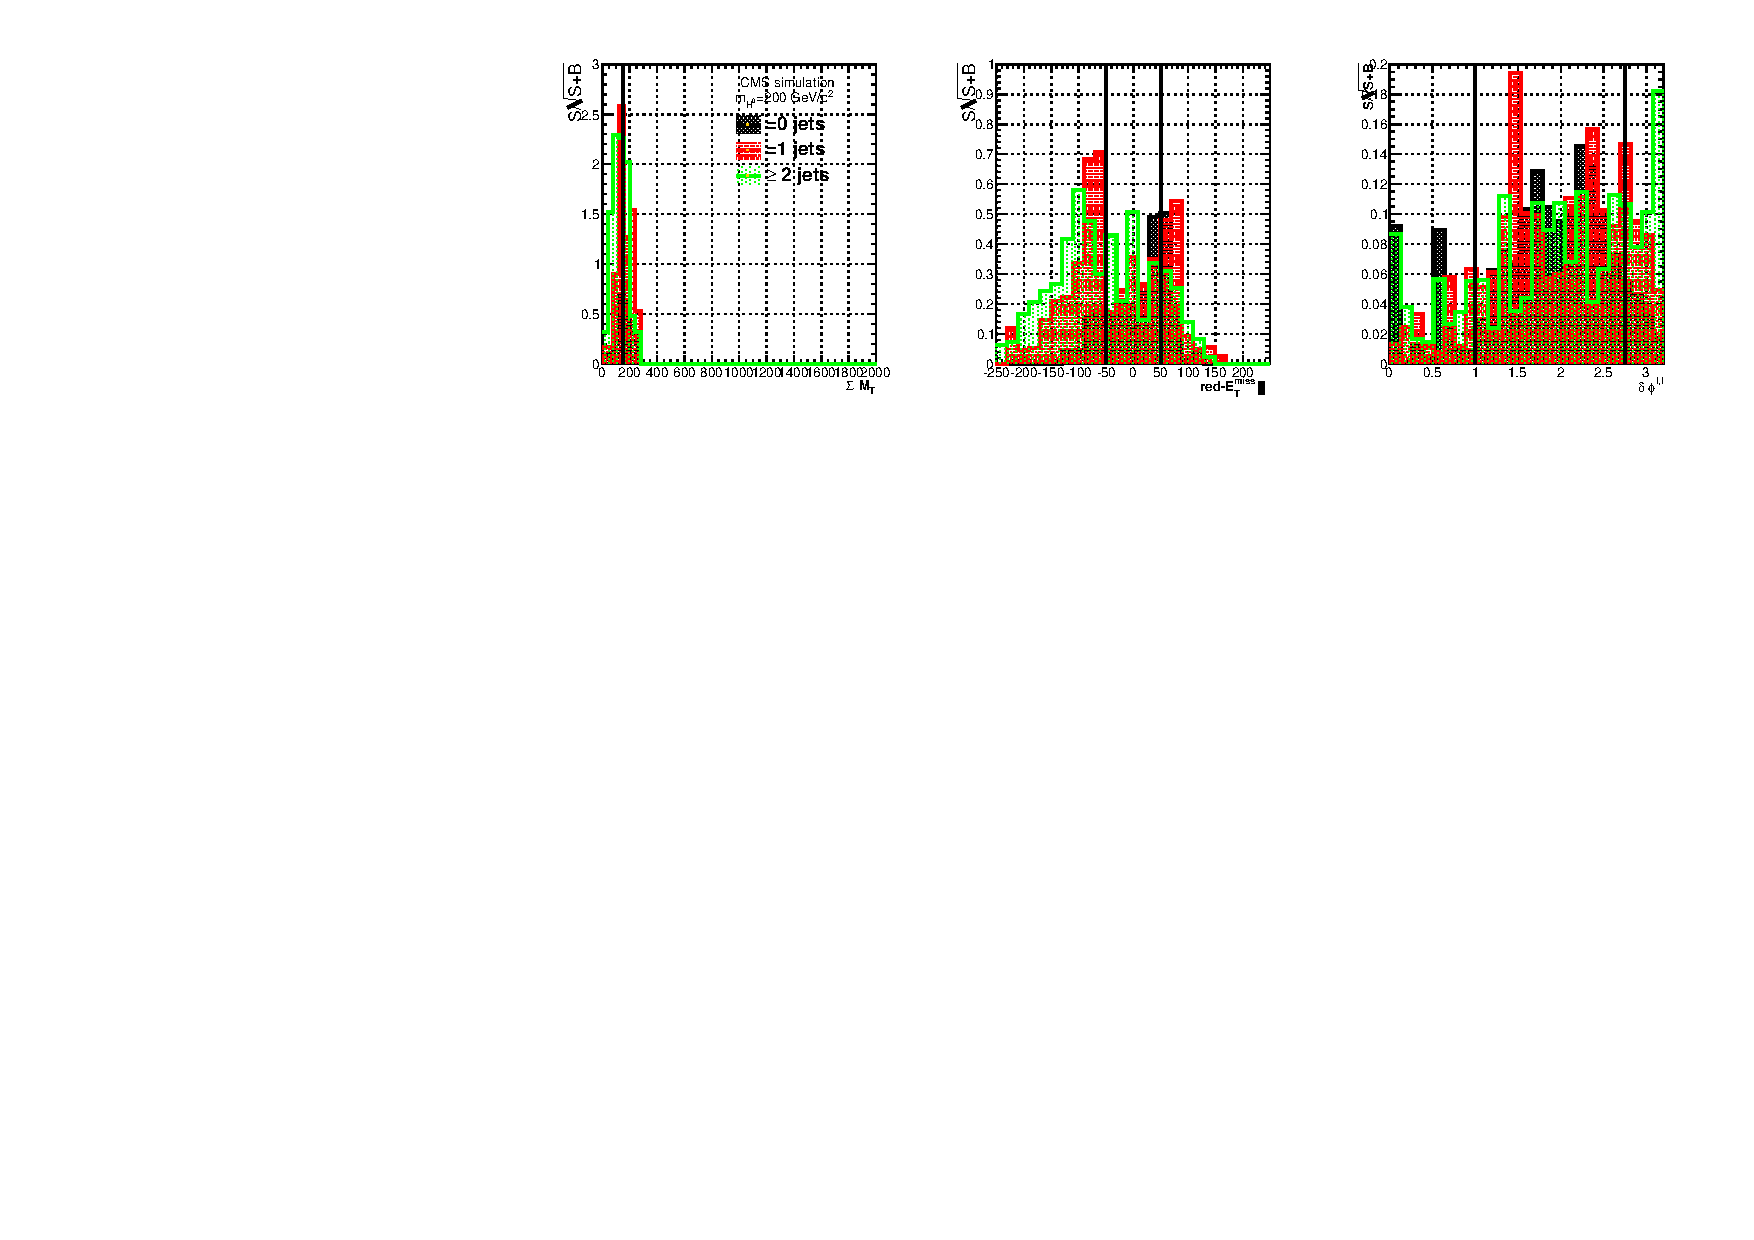
\includegraphics[width=0.64\textwidth]{img/FoM_200}\\
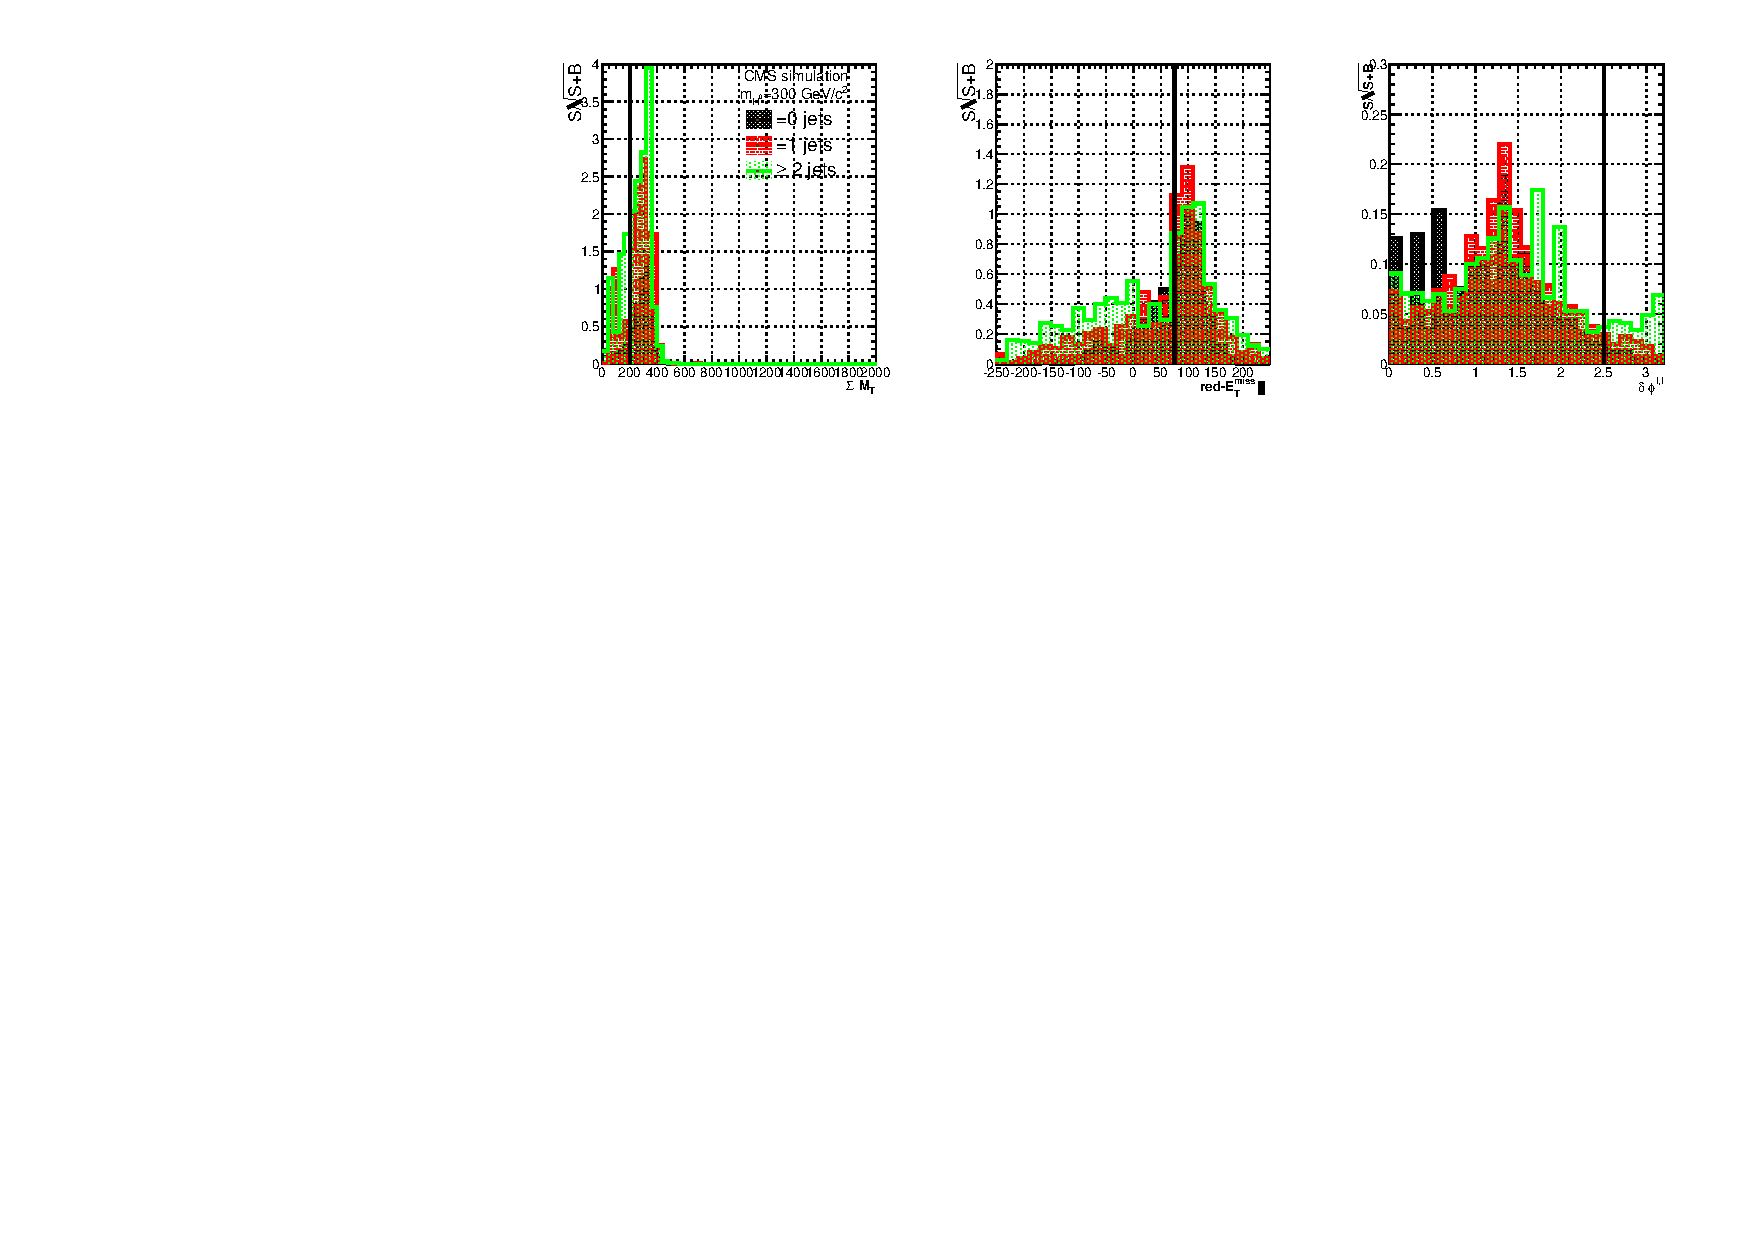
\includegraphics[width=0.64\textwidth]{img/FoM_300}\\
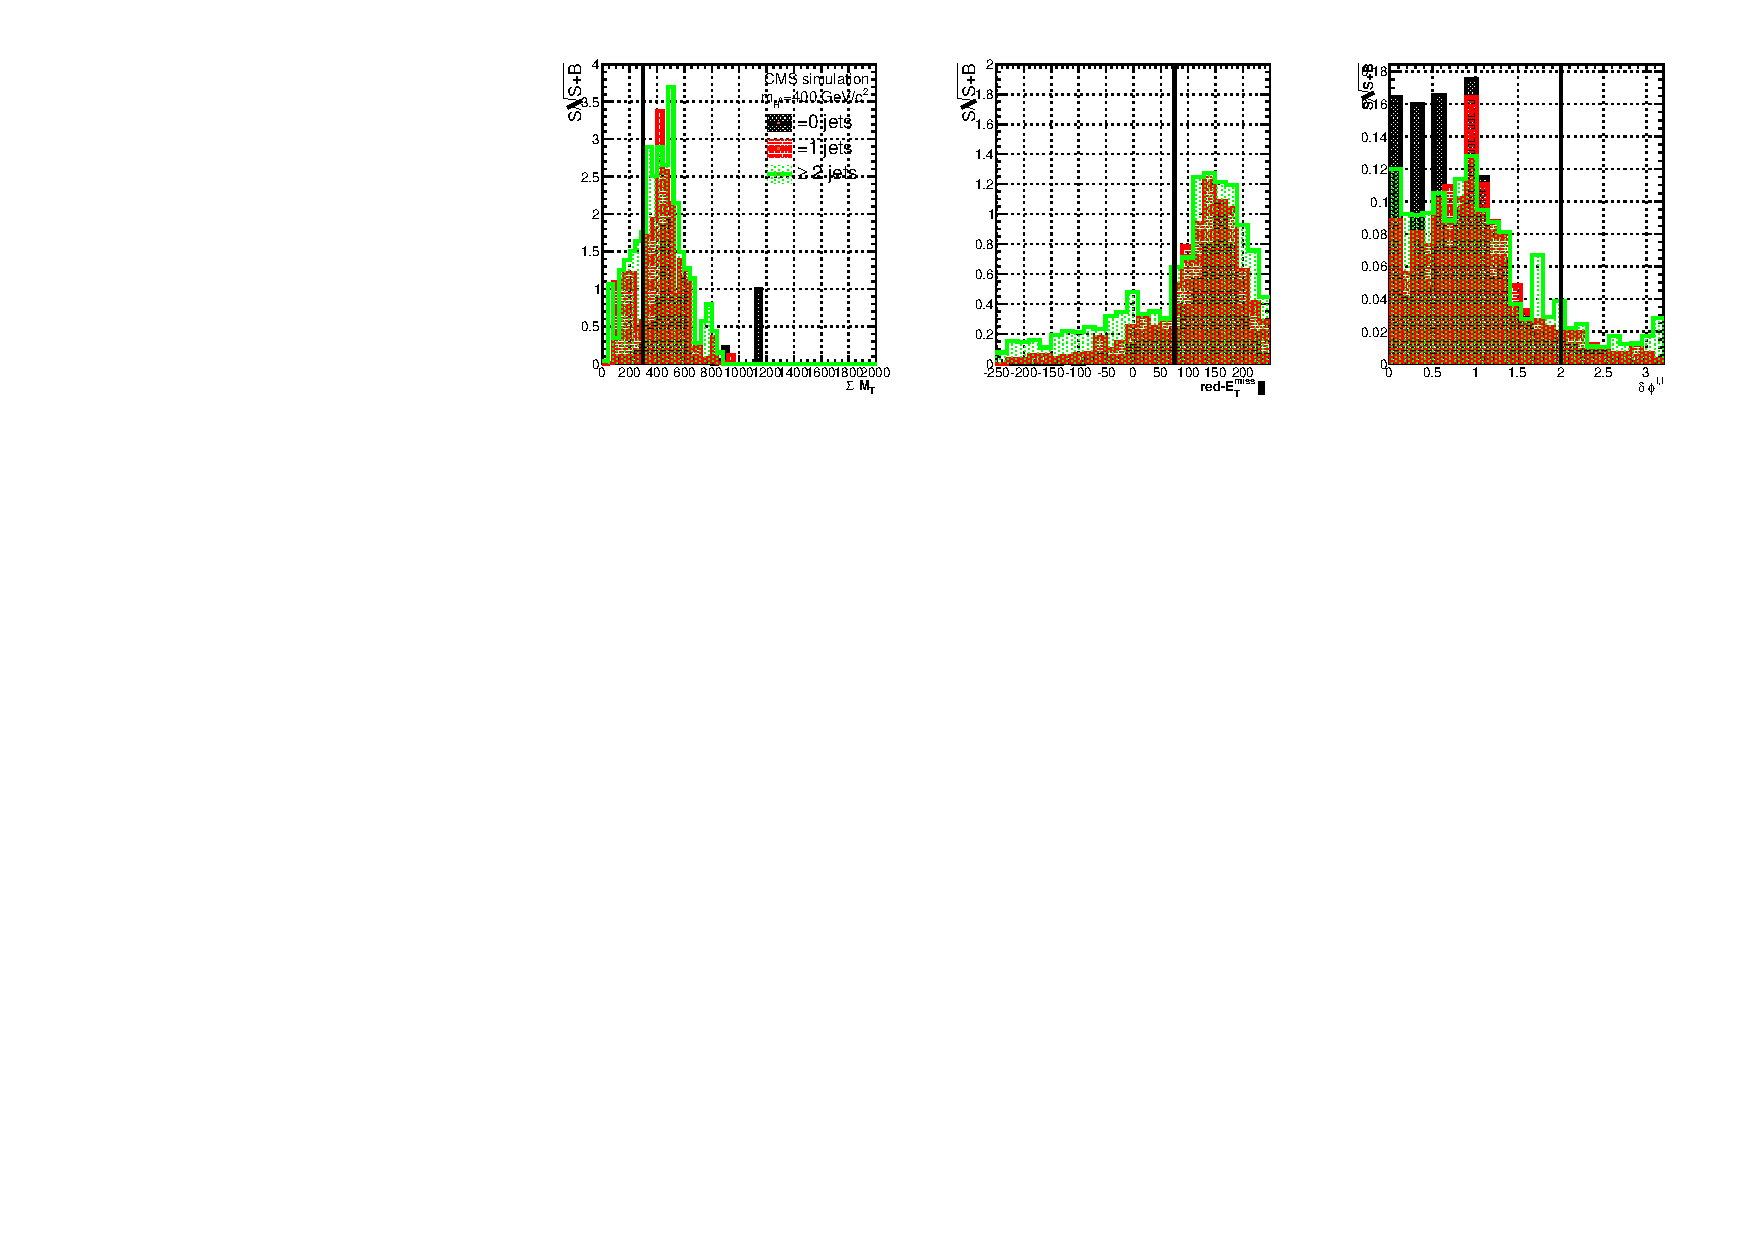
\includegraphics[width=0.64\textwidth]{img/FoM_400}\\
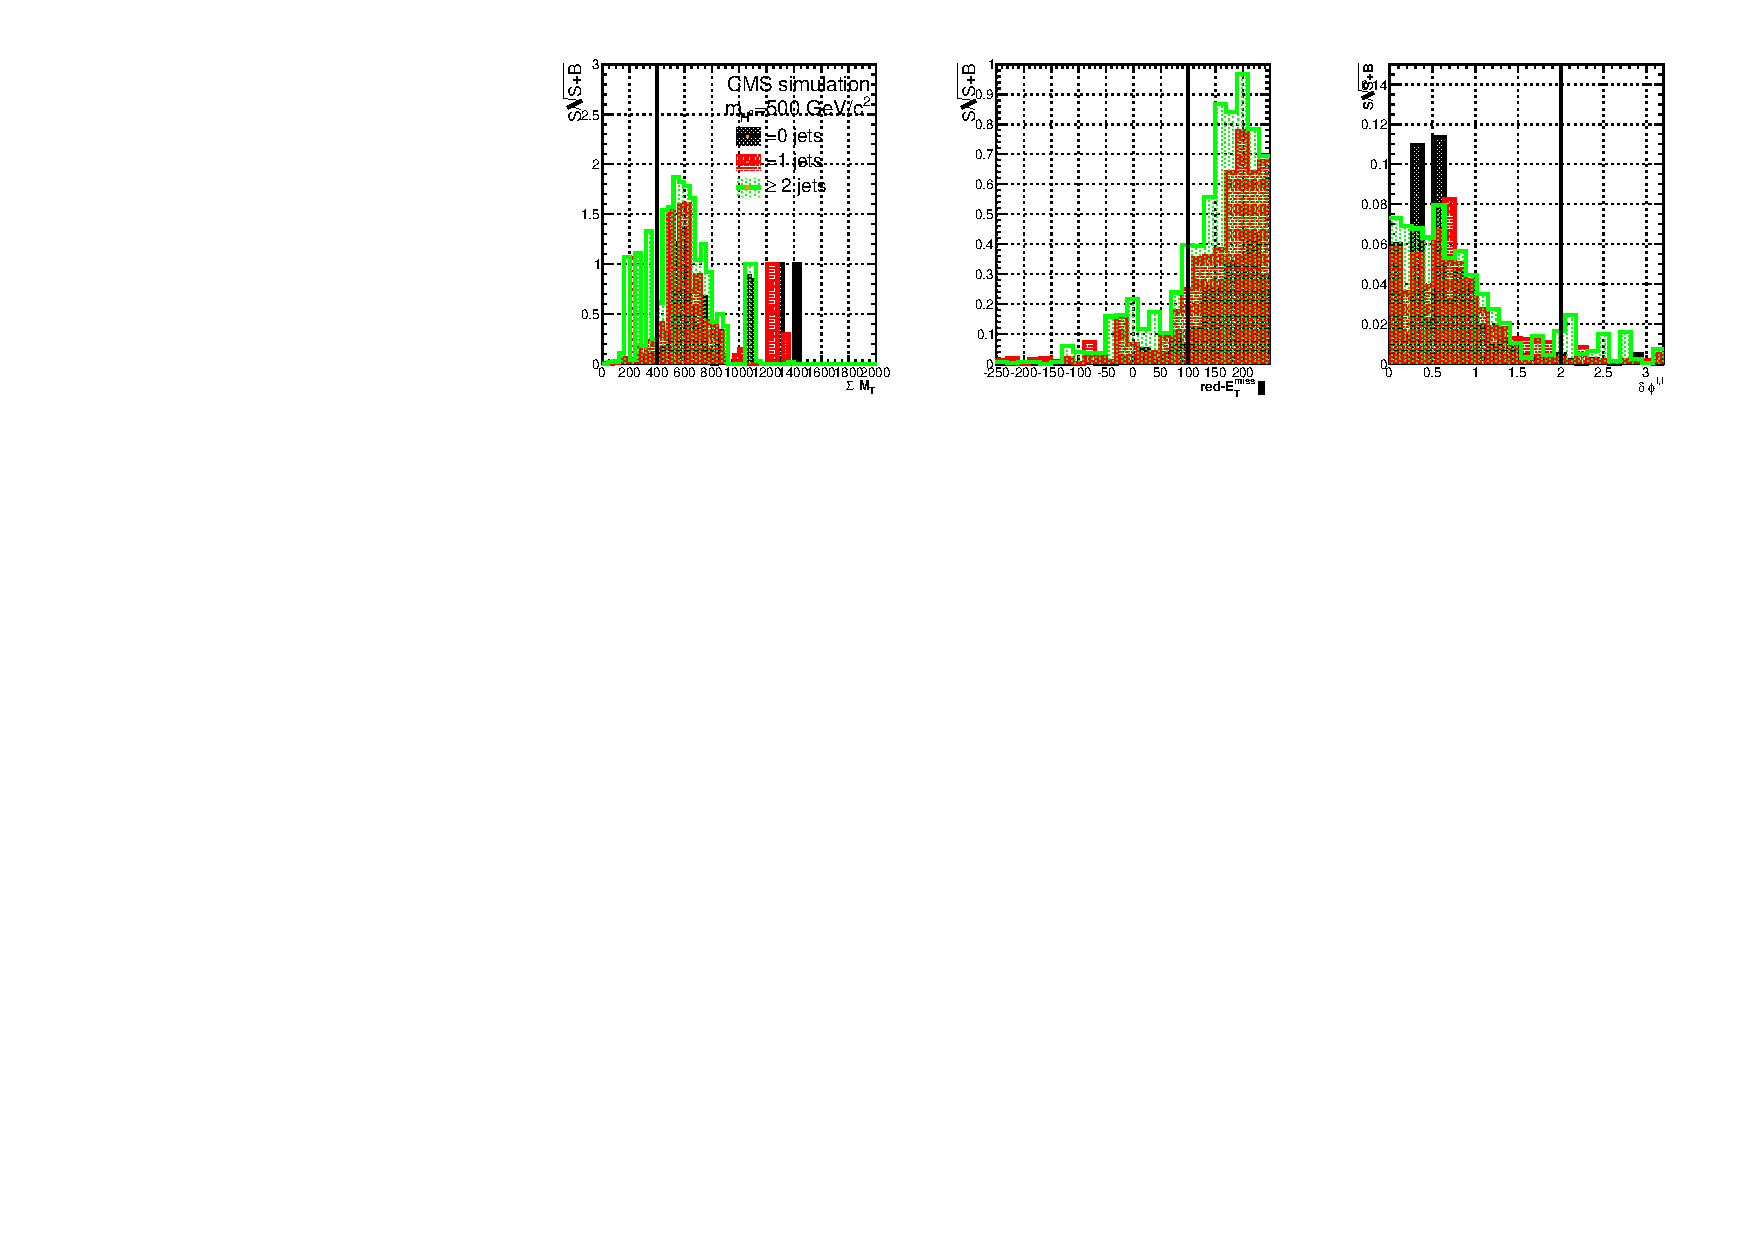
\includegraphics[width=0.64\textwidth]{img/FoM_500}\\
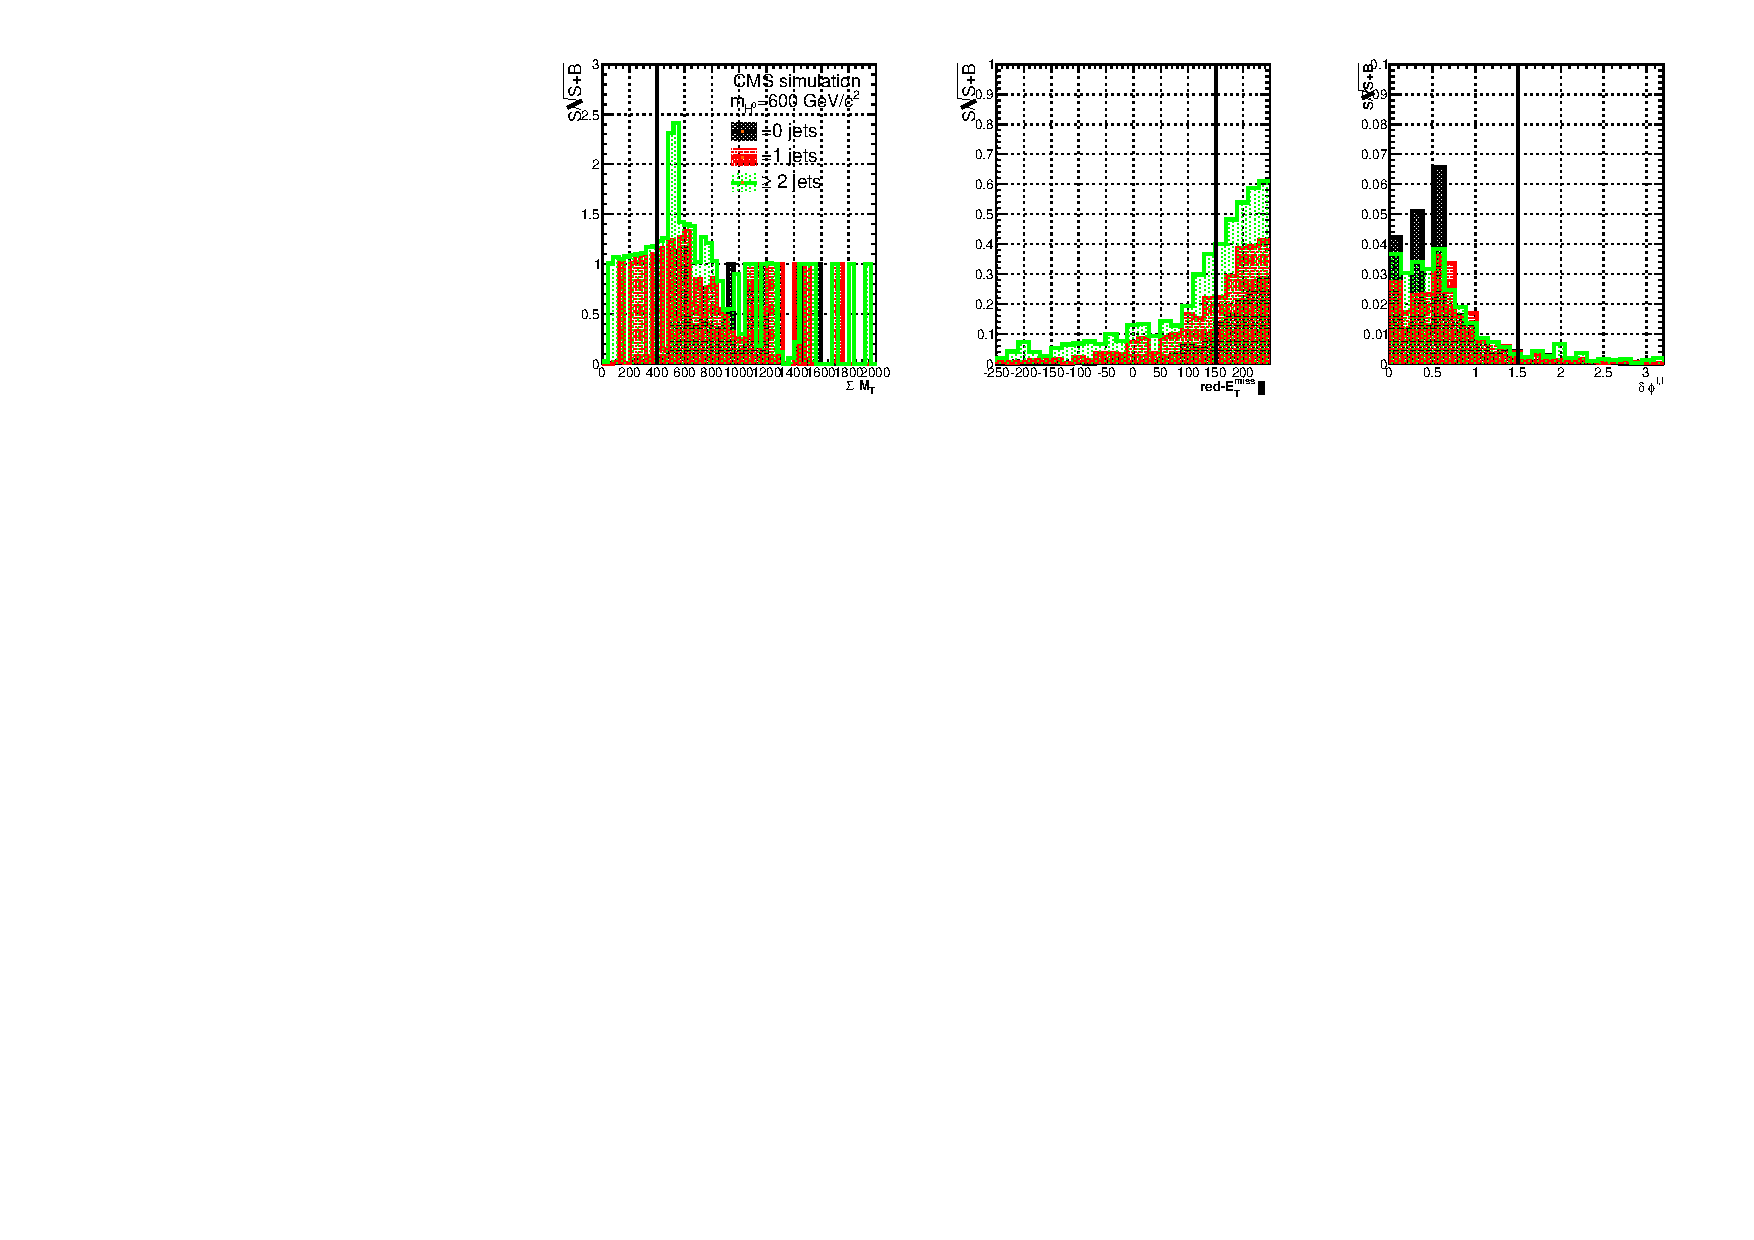
\includegraphics[width=0.64\textwidth]{img/FoM_600}
\caption{Figure of merit for different Higgs masses for different variables and for events with different jet multiplicities. 
The cut chosen for each variable is overlaid in the figures.
All backgrounds, as predicted by simulation, are considered.}
\label{fig:varcutopt}
\end{center}
\end{figure}

  
\end{document}


